\documentclass{report}
\usepackage{geometry}
\geometry{margin=1.05in}
\usepackage{amsmath}
\usepackage[makeroom]{cancel}
%\numberwithin{equation}{section}
\usepackage{graphicx}
\usepackage{float}
%\restylefloat{table}
\usepackage{subcaption}
\usepackage{empheq}
%\usepackage{slashbox}
\newcommand*\widefbox[1]{\fbox{\hspace{2em}#1\hspace{2em}}}
\usepackage{natbib}
\bibliographystyle{abbrvnat}
\usepackage{hyperref}
\usepackage{siunitx}
\usepackage[table,pdftex,dvipsnames]{xcolor}
\usepackage[titletoc]{appendix}
\usepackage{animate}
\usepackage{makecell}

\usepackage{multicol}
\hypersetup{
	colorlinks,
	linkcolor={red!50!black},
	citecolor={black},
	urlcolor={blue!80!black}
}
\graphicspath{{figures/}}
\DeclareMathOperator\sech{sech}
\DeclareMathOperator\erf{erf}
\DeclareMathOperator\erfc{erfc}
\graphicspath{{figures/}}
\usepackage{listings}
\usepackage{color}
\usepackage{ifthen}

\DeclareMathOperator{\sgn}{sgn}
\DeclareMathOperator{\re}{Re}
\DeclareMathOperator{\im}{Im}
\DeclareMathOperator{\Da}{Da}
\DeclareMathOperator{\erfi}{erfi}
\DeclareMathOperator{\atan2}{atan2}

\definecolor{dkgreen}{rgb}{0,0.6,0}
\definecolor{gray}{rgb}{0.5,0.5,0.5}
\definecolor{mauve}{rgb}{0.58,0,0.82}

\newcommand{\RN}[1]{\MakeUppercase{\romannumeral #1}}
%\lstset{frame=tb,
	%	language=Matlab,
	%	aboveskip=3mm,
	%	belowskip=3mm,
	%	showstringspaces=false,
	%	columns=flexible,
	%	basicstyle={\small\ttfamily},
	%	numbers=none,
	%	numberstyle=\tiny\color{gray},
	%	keywordstyle=\color{blue},
	%	commentstyle=\color{dkgreen},
	%	stringstyle=\color{mauve},
	%	breaklines=true,
	%	breakatwhitespace=true,
	%	tabsize=3
	%}
%

\lstset{language=[5.3]lua,
	%	backgroundcolor=\color{backcolour},   
	commentstyle=\color{OliveGreen},
	keywordstyle=\color{RoyalBlue},
	numberstyle=\tiny\color{Gray},
	stringstyle=\color{Orange},
	basicstyle=\footnotesize\ttfamily,
	breaklines=true, breakatwhitespace=true,     
	breaklines=true,                 
	captionpos=t,                    
	keepspaces=true,                 
	numbers=left,                    
	numbersep=5pt,                  
	showspaces=false,                
	showstringspaces=false,
	showtabs=false,                  
	tabsize=2,
	frame=tb,
	prebreak=\raisebox{0ex}[0ex][0ex]{\ensuremath{\hookleftarrow}},
	postbreak=\raisebox{0ex}[0ex][0ex]{\ensuremath{\space\hookrightarrow\space}},
}




\setlength{\textwidth}{6.5in}
\setlength{\textheight}{8.5in}
\setlength{\evensidemargin}{0in}
\setlength{\oddsidemargin}{0in}
\setlength{\topmargin}{0in}

\setlength{\parindent}{0pt}
\setlength{\parskip}{0.1in}

\usepackage[section]{placeins}

\let\Oldsubsection\subsection
\renewcommand{\subsection}{\FloatBarrier\Oldsubsection}

\let\Oldsubsubsection\subsubsection
\renewcommand{\subsubsection}{\FloatBarrier\Oldsubsubsection}


%%%%%%%%%%%%%%%% Notes and things to add:
% Maybe use widetilde instead of tilde
% Clean up this header section over here
% Double check all equation labels and references.



\title{O$^+$-O Collision Cross Section}
\author{Chirag R. Skolar}
\date{\today}

\begin{document}
	\maketitle
	
	\tableofcontents
	
	% Intro discussing problem. 
	
	% Some section on how the MC sims work. 
	
	% Discussion of theory on the collision cross section
	
	% Discussion of numerical integration used to get spectra
	
	% Put all the tests I've done in an appendix
	
	\chapter{Introduction}

\section{O+O Stuff}

\section{ISR Theory}
\label{s:ISR-spectra}
The scattering spectra, $S$, of an electromagnetic wave on a one ion species magnetized collisional plasma is
\begin{equation}
	S(\omega,\mathbf{k}) = 2 \Big| 1 - \frac{\chi_e}{\epsilon}\Big|^2
	+ 2\Big|\frac{\chi_e}{\epsilon}\Big|^2 M_i,
	\label{eq:scatterin-spectra}
\end{equation}
where $\chi$ is the susceptibility, 
$M$ is the modified distribution function,
and $\epsilon$ is the dielectric function defined as
\begin{equation}
	\epsilon = 1 + \chi_e + \chi_i.
\end{equation}
To obtain these values, we first need to calculate the collisional term, $U_s$. % Include something on the collisional terms
For a species $s$ with normalized distribution function $f_{0s}(v)$, the 
\begin{equation}
	U_s = i \nu_s \sum_n \int 
	\frac{J_n^2\Big( \tfrac{k_\perp v_\perp}{\Omega_{cs}} \Big)}
	{\omega - k_\parallel v_\parallel - n\Omega_{cs} - i\nu_s}  
	f_{0s}(v)   d\mathbf{v}^3 ,
\end{equation}
where $\nu$ is the total collision frequency,
$\Omega_{c}$ is the gyrofrequency,
$J_n$ is the $n$-th order Bessel function of the first kind,
and the integrals are taken over all velocity space.
The susceptibility is
\begin{equation}
	\chi_s = \frac{\omega_p^2}{k^2(1+U_s)} \sum_n \int 
	\frac{J_n^2\Big( \tfrac{k_\perp v_\perp}{\Omega_{cs}} \Big)}
	{\omega - k_\parallel v_\parallel - n\Omega_{cs} - i\nu_s}  
	\mathbf{k} \cdot \frac{\partial f_{0s}}{\partial \mathbf{v}}   d\mathbf{v}^3 ,
\end{equation} 
where $\omega_p$ is the plasma frequency
and the derivative term is defined as
\begin{equation}
	\mathbf{k} \cdot \frac{\partial f_{0s}}{\partial \mathbf{v}} = 
	k_\parallel \frac{\partial f_{0s}}{\partial v_\parallel}
	+ \frac{n \Omega_{cs}}{v_\perp} \frac{\partial f_{0s}}{\partial v_\perp}.
\end{equation}
The modified distribution function is 
\begin{equation}
	M_s = \frac{\nu_s}{|1+U_s|^2}
	\Bigg( - \frac{|U_s|^2}{\nu_s^2} 
	+ \sum_n \int 
	\frac{J_n^2\Big( \tfrac{k_\perp v_\perp}{\Omega_{cs}} \Big)}
	{(\omega - k_\parallel v_\parallel - n\Omega_{cs})^2 + \nu_s^2}
	f_{0s}(v)   d\mathbf{v}^3 \Bigg).
\end{equation}

For a normalized Maxwellian distribution,
\begin{equation}
	f_{0s} = 
	\frac{1}{v_{th,s}^3\pi^{3/2}}
	\exp\bigg[- \frac{(v_\perp^2 + v_\parallel^2)}{v_{th,s}^2} \bigg],
\end{equation}
the collisional term, susceptibility, and modified distribution function are
\begin{equation}
	U_s = 
	\frac{i \nu_{s}}{k_\parallel v_{th,s}} 
	\sum_n \exp(-k_\perp^2 \bar{\rho}_s^2) I_n (k_\perp^2 \bar{\rho}_s^2) 
	\Big[ 2 \Da(y_n) + i \sqrt{\pi} \exp(-y_n^2) \Big]
\end{equation}
\begin{equation}
	\chi_s = 
	\frac{\alpha^2}{1+U_s} \frac{T_e}{T_s} 
	\sum_n \exp(-k_\perp^2 \bar{\rho}_s^2) I_n (k_\perp^2 \bar{\rho}_s^2) 
	\bigg[ 1 - \frac{\omega-i\nu_s}{k_\parallel v_{th,s}} 
	\Big( 2 \Da[y_n] + i \sqrt{\pi} \exp[-y_n^2] \Big)
	\bigg]
\end{equation}
\begin{equation}
	M_s = 
	\Bigg[
	\frac{1}{|1+U_s|^2} \frac{\sqrt{\pi}}{k_\parallel v_{th,s}}
	\sum_n \exp(-k_\perp^2 \bar{\rho}_s^2) I_n (k_\perp^2 \bar{\rho}_s^2) \exp(-y_n^2)
	\Bigg]
	- \frac{|U_s|^2}{\nu_s |1+U_s|^2},
\end{equation}
where
\begin{equation}
	y_n = \frac{\omega-n\Omega_{cs}-i\nu_s}{k_\parallel v_{th,s}}
\end{equation}
\begin{equation}
	\bar{\rho}_s = \frac{v_{th,s}}{\sqrt{2}\Omega_{cs}}
\end{equation}
\begin{equation}
	\alpha = \frac{1}{k \lambda_{D_e}}.
\end{equation}
See Appendix~\ref{a:spectra} for the full derivation.


	
	\chapter{Numerical Methods}

\section{Monte Carlo}

A discussion of the Monte Carlo methods here



\section{Incoherent Scatter Spectra Calculation}

\subsection{Obtaining $M_s$ and $\chi_s$}

The incoherent scatter spectra of a plasma is calculated using Eq.~\ref{eq:scattering-spectra}, which needs Eqs.~\ref{eq:dielectric}-\ref{eq:Ms}.
For an arbitrary distribution function, it is difficult to calculate this, especially when the distribution function does not have an analytical form (like that of a Monte Carlo output).
\cite{goodwin2018} provide a method involving applying several curve fitting techniques to the ion distribution function. 
This method provides good results but requires significant input from the user to ensure a good fit. % Double check this statement. 
The primary reason for these techniques was to have minimal noise in the derivative of the distribution, as used in Eq.~\ref{eq:chis} and described in Eq.~\ref{eq:chis_derivative}.
Furthermore, the spectrum calculation in \citep{goodwin2018} assumes tha the ions are entirely unmagnetized. 
We will provide a different method with no input from the user (beyond choosing the initial velocity mesh extent and resolution) that fully include the effects of collisions and magnetic fields.


To simplify the calculation, we assume that the distribution function is axisymmetric in velocity space about the axis parallel to the magnetic field. 
Thus, cylindrical coordinates are the natural choice with the velocity space discretized by $v_\parallel$ and $v_\perp$ and the azimuth angle described by $\phi$.
The integral over all velocity space of an arbitrary function $f$ in cylindrical coordiantes is
\begin{equation}
	\int f(\mathbf{v}) d\mathbf{v} = \int_0^\infty  dv_\perp v_\perp  \int_{-\infty}^\infty dv_\parallel \int_0^{2\pi} f(v_\perp, v_\parallel) d\phi.
	\label{eq:cylindrical_integration}
\end{equation}
Due to azimuthal symmetry, the integral over $\phi$ just becomes $2\pi$ yielding
\begin{equation}
	\int f(\mathbf{v}) d\mathbf{v} = 2\pi \int_0^\infty  dv_\perp v_\perp  \int_{-\infty}^\infty f(v_\perp, v_\parallel)  dv_\parallel.
	\label{eq:cylind_int_2pi}
\end{equation}


Eq.~\ref{eq:cylind_int_2pi} can be applied to the calculation of $U_s$, $M_s$, and $\chi_s$. 
Let us begin with $U_s$. We can rewrite the denominator to be $v_\parallel-z$ where 
\begin{equation}
	z = \frac{\omega - n\Omega_{cs}- i \nu_s}{k_\parallel}.
	\label{eq:z}
\end{equation}
Using Eqs.~\ref{eq:cylind_int_2pi} and \ref{eq:z}, Eq.~\ref{eq:Us} becomes
\begin{equation}
	U_s = - \frac{2 \pi i \nu_s}{k_\parallel} \sum_n 
	\int_0^\infty dv_\perp v_\perp J_n^2 \bigg( \frac{k_\perp v_\perp}{\Omega_{cs}} \bigg)
	\int_{-\infty}^\infty  
	\frac{f_{0s}(v_\perp, v_\parallel)}{v_\parallel - z} dv_\parallel
	\label{eq:Us_final}
\end{equation}


For $M_s$, the denominator term can similarly be rewritten as $(v_\parallel-z)(v_\parallel-z^*)$
where $z^*$ is the complex conjugate of $z$.
Therefore, Eq.~\ref{eq:Ms} can be rewritten as  % Revisit this calculation and make sure I'm doing it correctly. I feel like to do it right, I need a kpar^2 in the outside denominator
\begin{equation}
	M_s = \frac{\nu_s}{|1+U_s|^2} 
	\Bigg[ -\frac{|U_s|^2}{\nu_s^2} 
	+ \frac{1}{k_\parallel^2}\sum_n \int_0^\infty   dv_\perp v_\perp J_n^2 \bigg( \frac{k_\perp v_\perp}{\Omega_{cs}} \bigg)
	\int_{-\infty}^\infty \frac{f_{0s}(v_\perp, v_\parallel)}{(v_\parallel - z)(v_\parallel - z^*)} dv_\parallel
	\Bigg]
	\label{eq:Ms_final}
\end{equation}


The denominator term for the magnetized susceptibility, $\chi_s$, can also be rewritten as $v_\parallel-z$, just as we did for $U_s$ in Eq.~\ref{eq:Us_final}.
Therefore, Eq.~\ref{eq:chis} can be rewritten as
\begin{equation}
	\chi_s = -\frac{\omega_{ps}^2}{k_\parallel k^2 (1+U_s)} \sum_n \int d\mathbf{v}^3 
	 \frac{ J_n^2\Big( \frac{k_\perp v_\perp}{\Omega_{cs}}\Big)  }{v_\parallel-z}
	\bigg( k_\parallel \frac{\partial}{\partial v_\parallel} + \frac{n\Omega_{cs}}{v_\perp} \frac{\partial }{\partial v_\perp}  \bigg) f_{0s}(v_\perp, v_\parallel) .
	\label{eq:chis_denom}
\end{equation}
Let us split this integral into two integrals based on the derivatives:
\begin{align}
	\chi_s^\parallel &= -\frac{\omega_{ps}^2}{k^2 (1+U_s)} \sum_n \int d\mathbf{v}^3 
	\frac{ J_n^2\Big( \frac{k_\perp v_\perp}{\Omega_{cs}}\Big)  }{v_\parallel-z}
	\frac{\partial}{\partial v_\parallel} f_{0s}(v_\perp, v_\parallel)
	\label{eq:chis_par} \\
	\chi_s^\perp &= -\frac{\omega_{ps}^2}{k_\parallel k^2 (1+U_s)} \sum_n \int d\mathbf{v}^3 
	\frac{ J_n^2\Big( \frac{k_\perp v_\perp}{\Omega_{cs}}\Big)  }{v_\parallel-z}
	\frac{n\Omega_{cs}}{v_\perp} \frac{\partial }{\partial v_\perp} f_{0s}(v_\perp, v_\parallel).
	\label{eq:chis_perp}
\end{align}
These derivatives are difficult to deal with numerically.
So, we want to use integration by parts to move the derivative from the distribution function to other things that we already know the analytical derivatives of.

First, we look at the parallel susceptibility.
In cylindrical coordinates, it becomes
\begin{equation}
	\chi_s^\parallel = -\frac{2\pi \omega_{ps}^2}{k^2 (1+U_s)} \sum_n 
	\int_0^\infty dv_\perp v_\perp J_n^2 \bigg( \frac{k_\perp v_\perp}{\Omega_{cs}}  \bigg)
	\int_{-\infty}^\infty \frac{1}{v_\parallel-z} 
	\frac{\partial}{\partial v_\parallel} f_{0s}(v_\perp, v_\parallel).
	\label{eq:chis_par_cylind}
\end{equation} 	
Using integration by parts, the parallel integral becomes
\begin{equation}
	\int_{-\infty}^\infty \frac{1}{v_\parallel-z} 
	\frac{\partial}{\partial v_\parallel} f_{0s}(v_\perp, v_\parallel) = 
	\frac{f_{0s}(v_\parallel,v_\perp)}{v_\parallel-z}\bigg|_{-\infty}^\infty
	- \int_{-\infty}^\infty dv_\parallel f_{0s}(v_\perp, v_\parallel)
	\frac{\partial}{\partial v_\parallel} \bigg( \frac{1}{v_\parallel-z}  \bigg).
	\label{eq:par_int_parts}
\end{equation}
The boundary term is zero because the distribution function tends to 0 at $\pm \infty$.
The remaining derivative is straightforward to calculate resulting in a parallel integral of 
\begin{equation}
	\int_{-\infty}^\infty \frac{1}{v_\parallel-z} 
	\frac{\partial}{\partial v_\parallel} f_{0s}(v_\perp, v_\parallel) = 
	\int_{-\infty}^\infty \frac{f_{0s}(v_\perp, v_\parallel)}{(v_\parallel-z)^2}  dv_\parallel.
	\label{eq:par_int_parts_final}
\end{equation}
Substituting Eq.~\ref{eq:par_int_parts_final} into Eq.~\ref{eq:chis_par_cylind} gives a parallel susceptibility of
\begin{equation}
	\chi_s^\parallel = -\frac{2\pi \omega_{ps}^2}{k^2 (1+U_s)} \sum_n 
	\int_0^\infty dv_\perp v_\perp J_n^2 \bigg( \frac{k_\perp v_\perp}{\Omega_{cs}}  \bigg)
	\int_{-\infty}^\infty \frac{f_{0s}(v_\perp, v_\parallel)}{(v_\parallel-z)^2} dv_\parallel.
	\label{eq:chis_par_final}
\end{equation}

Now, let us look at the perpendicular integral. In cylindrical coordinates, Eq.~\ref{eq:chis_perp} is
\begin{equation}
	\chi_s^\perp = -\frac{2\pi \omega_{ps}^2}{k_\parallel k^2 (1+U_s)} \sum_n
	n \Omega_{cs} 
	\int_{-\infty}^\infty \frac{dv_\parallel}{v_\parallel - z} 
	\int_0^\infty J_n^2 \bigg( \frac{k_\perp v_\perp}{\Omega_{cs}}  \bigg)
	\frac{\partial }{\partial v_\perp} f_{0s}(v_\perp, v_\parallel) dv_\perp.
	\label{eq:chis_perp_cylind}
\end{equation}
Note that the order of integration has been switched compared to the other cases we have been doing. 
And note that the $v_\perp$ term in the perpendicular derivative in Eq.~\ref{eq:chis_derivative} is cancelled by the multiplied $v_\perp$ term for cylindrical integration in Eq.~\ref{eq:cylind_int_2pi}.
Looking at just the perpendicular integral and integrating by parts, we get
\begin{equation}
	\int_0^\infty J_n^2 \bigg( \frac{k_\perp v_\perp}{\Omega_{cs}}  \bigg)
	\frac{\partial }{\partial v_\perp} f_{0s}(v_\parallel,v_\perp) dv_\perp = 
	J_n^2 \bigg( \frac{k_\perp v_\perp}{\Omega_{cs}}  \bigg) f_{0s}(v_\perp, v_\parallel)\bigg|_0^\infty
	-\int_0^\infty dv_\perp f_{0s}(v_\perp, v_\parallel)
	\frac{\partial}{\partial v_\perp} \Bigg[  
	J_n^2 \bigg( \frac{k_\perp v_\perp}{\Omega_{cs}}  \bigg)
	\Bigg]
	\label{eq:perp_int_parts}
\end{equation}
For the boundary term, the distribution function is again 0 at $\infty$ so the upper bound goes to zero.
The lower bound, however, is non-zero and evaluates to 
\begin{equation}
	J_n^2 \bigg( \frac{k_\perp v_\perp}{\Omega_{cs}}  \bigg) f_{0s}(v_\perp, v_\parallel)\bigg|_0^\infty
	= J_n^2(0) f_{0s}(0, v_\parallel).
	\label{eq:perp_int_boundary}
\end{equation}
For $n\neq0$, the Bessel function $J_n$ evaluates to 0.
Thus, a boundary term only exists for $n=0$ where $J_0(0)=1$.
But conveniently, the entirety of the perpendicular susceptibility is multiplied by $n$ as shown in Eq.~\ref{eq:chis_perp_cylind}.
So for $n=0$ the perpendicular suceptilibity is 0 and thus we do not need to consider the boundary term at all.

This leaves the derivative term in Eq.~\ref{eq:perp_int_parts} which (from Mathematica) is
\begin{equation}
	\frac{\partial}{\partial v_\perp} \Bigg[  
	J_n^2 \bigg( \frac{k_\perp v_\perp}{\Omega_{cs}}  \bigg) \Bigg]= 
	\frac{k_\perp}{\Omega_{cs}} J_n \bigg( \frac{k_\perp v_\perp}{\Omega_{cs}}  \bigg)
	\Bigg[ 
	J_{n-1} \bigg( \frac{k_\perp v_\perp}{\Omega_{cs}}  \bigg)
	-J_{n+1} \bigg( \frac{k_\perp v_\perp}{\Omega_{cs}}  \bigg)
	\Bigg].
	\label{eq:perp_int_parts_deriv}
\end{equation} 
Thus, plugging Eq.~\ref{eq:perp_int_parts_deriv} into Eq.~\ref{eq:perp_int_parts} and setting the boundary term to zero yields
\begin{equation}
	\int_0^\infty J_n^2 \bigg( \frac{k_\perp v_\perp}{\Omega_{cs}}  \bigg)
	\frac{\partial }{\partial v_\perp} f_{0s}(v_\perp, v_\parallel) dv_\perp = 
	-\frac{k_\perp}{\Omega_{cs}} 
	\int_0^\infty dv_\perp f_{0s}(v_\perp, v_\parallel)
	J_n \bigg( \frac{k_\perp v_\perp}{\Omega_{cs}}  \bigg)
	\Bigg[ 
	J_{n-1} \bigg( \frac{k_\perp v_\perp}{\Omega_{cs}}  \bigg)
	-J_{n+1} \bigg( \frac{k_\perp v_\perp}{\Omega_{cs}}  \bigg)
	\Bigg].
	\label{eq:perp_int_parts_final}
\end{equation}
Thus, the perpendicular susceptibility term is
\begin{equation}
	\chi_s^\perp = \frac{2\pi \omega_{ps}^2 k_\perp}{k_\parallel k^2 (1+U_s)} \sum_n
	n 
	\int_{0}^\infty dv_\perp J_n \bigg( \frac{k_\perp v_\perp}{\Omega_{cs}}  \bigg)
	\Bigg[ 
	J_{n-1} \bigg( \frac{k_\perp v_\perp}{\Omega_{cs}}  \bigg)
	-J_{n+1} \bigg( \frac{k_\perp v_\perp}{\Omega_{cs}}  \bigg)
	\Bigg]
	\int_{-\infty}^\infty \frac{f_{0s}(v_\perp, v_\parallel)}{v_\parallel-z} dv_\parallel.
	\label{eq:chis_perp_final}
\end{equation}
Note that it is useful from a numerical perspective to do the parallel integration first,
so we switched the order of integration.

Combining the parallel and perpendicular susceptibilities (Eqs.~\ref{eq:chis_par_final} and \ref{eq:chis_perp_final}) yields
\begin{multline}
	\chi_s = \chi_s^\parallel + \chi_s^\perp = 
	\frac{2\pi \omega_{ps}^2}{k^2 (1+U_s)}	\sum_n
	\Bigg\{ - \int_0^\infty dv_\perp v_\perp J_n^2 \bigg( \frac{k_\perp v_\perp}{\Omega_{cs}}  \bigg) 
	\int_{-\infty}^\infty \frac{f_{0s}(v_\perp, v_\parallel)}{(v_\parallel-z)^2} dv_\parallel \\
	+ \frac{nk_\perp}{k_\parallel} \int_0^\infty dv_\perp J_n \bigg( \frac{k_\perp v_\perp}{\Omega_{cs}}  \bigg)
	\Bigg[ 
	J_{n-1} \bigg( \frac{k_\perp v_\perp}{\Omega_{cs}}  \bigg)
	-J_{n+1} \bigg( \frac{k_\perp v_\perp}{\Omega_{cs}}  \bigg)
	\Bigg]
	\int_{-\infty}^\infty \frac{f_{0s}(v_\perp, v_\parallel)}{v_\parallel-z} dv_\parallel
	\Bigg\}
	\label{eq:chis_final}
\end{multline}

\subsection{Evaluating Pole Integrals}

From Eqs.~\ref{eq:Us_final}, \ref{eq:Ms_final}, and \ref{eq:chis_final}, we can calculate the resulting incoherent scatter spectrum using Eq.~\ref{eq:scattering-spectra}
However, these equations have difficult poles to deal with. 
They fall into the following three forms:
\begin{align}
	&\int_{-\infty}^\infty \frac{f_{0s}(v_\perp, v_\parallel)}{v_\parallel-z} dv_\parallel
	\label{eq:p1} \\
	&\int_{-\infty}^\infty \frac{f_{0s}(v_\perp, v_\parallel)}{(v_\parallel-z)(v_\parallel-z^*)} dv_\parallel 
	\label{eq:pstar}  \\
	&\int_{-\infty}^\infty \frac{f_{0s}(v_\perp, v_\parallel)}{(v_\parallel-z)^2} dv_\parallel
	\label{eq:p2} 
\end{align}
For a normalized one dimensional Maxwellian distribution of the form
\begin{equation}
	f_{0s} = \exp(\tilde{v}_\parallel^2),
	\label{eq:norm_maxwellian}
\end{equation}
where $\tilde{v}_\parallel$ is the parallel velocity normalized by the thermal velocity,
the analytical solutions for Eqs.~\ref{eq:p1}-\ref{eq:p2}, for an arbitrary pole $z$, are
\begin{align}
	p_1(z) &= \int_{-\infty}^\infty \frac{\exp(\tilde{v}_\parallel^2)}{\tilde{v}_\parallel-z} d\tilde{v}_\parallel 
	= \exp(-z^2) \Bigg[ -\pi \erfi(z) + \ln\bigg(\frac{1}{z}\bigg) + \ln(z)  \Bigg]
	\label{eq:p1Exact} \\
	p_*(z) &= \int_{-\infty}^\infty \frac{\exp(\tilde{v}_\parallel^2)}{(\tilde{v}_\parallel-z)(\tilde{v}_\parallel-z^*)} d\tilde{v}_\parallel 
	= \frac{i}{2\im(z)} \bigg[ p_1(z^*) - p_1(z) \bigg] 
	\label{eq:pstarExact} \\
	p_2(z) &= \int_{-\infty}^\infty \frac{\exp(\tilde{v}_\parallel^2)}{(\tilde{v}_\parallel-z)^2} d\tilde{v}_\parallel
	= - 2 \sqrt{\pi} - 2 p_1(z). 
	\label{eq:p2Exact}
\end{align}
For more information on how these were found, please see Appendix~\ref{a:poleIntegrals_Maxwellian} and the Mathematica notebook \verb*|exact_poleIntegrate.nb|.


For non-Maxwellian distributions, however, these integrals are much more difficult to handle and likely do not have an analytical solution.
In that case, we must find a method to numerically approximate the Eqs.~\ref{eq:p1}-\ref{eq:p2}.
\cite{longley2024} developed a mesh refinement algorithm about the poles to obtain a solution.
Here, we present a more accurate and intuitive method of solving these integrals. 


Figure~\ref{f:explainIntegrationMethod} provides an understanding of how we can numerically approximate the pole integrals.
Consider the Maxwellian from Eq.~\ref{eq:norm_maxwellian}, as is shown in the blue line.
The black dots are a discrete representation (from Monte Carlo, PIC, spectral, etc.) of this Maxwellian with a symmetric parallel velocity
mesh from $-4v_\parallel/v_{th}$ to $4v_\parallel/v_{th}$ with a $\Delta v_\parallel/v_{th}$ of 1.
As one can see, this is a very coarse mesh. 
The vertical dashed black line corresponds to the real part of the pole: in this case chosen to be $z=0.25+10^{-3}i$.
The discrete representation by itself does not do a good job of capturing the pole.
The red dots represent the linearly interpolated distribution function at a set of refined velocity points based on the algorithm by \cite{longley2024}.
These points, visually, provide a better approximation of the distribution function.
However, as will be shown in a few figures below, we found that this method was lacking, especially in terms of accurately capturing the second order pole, Eq.~\ref{eq:p2}.


% Add something about elements vs nodes here? Elemts from 0 to m, nodes go from 0 to m+1
\begin{figure}[!htb]
	\centering
	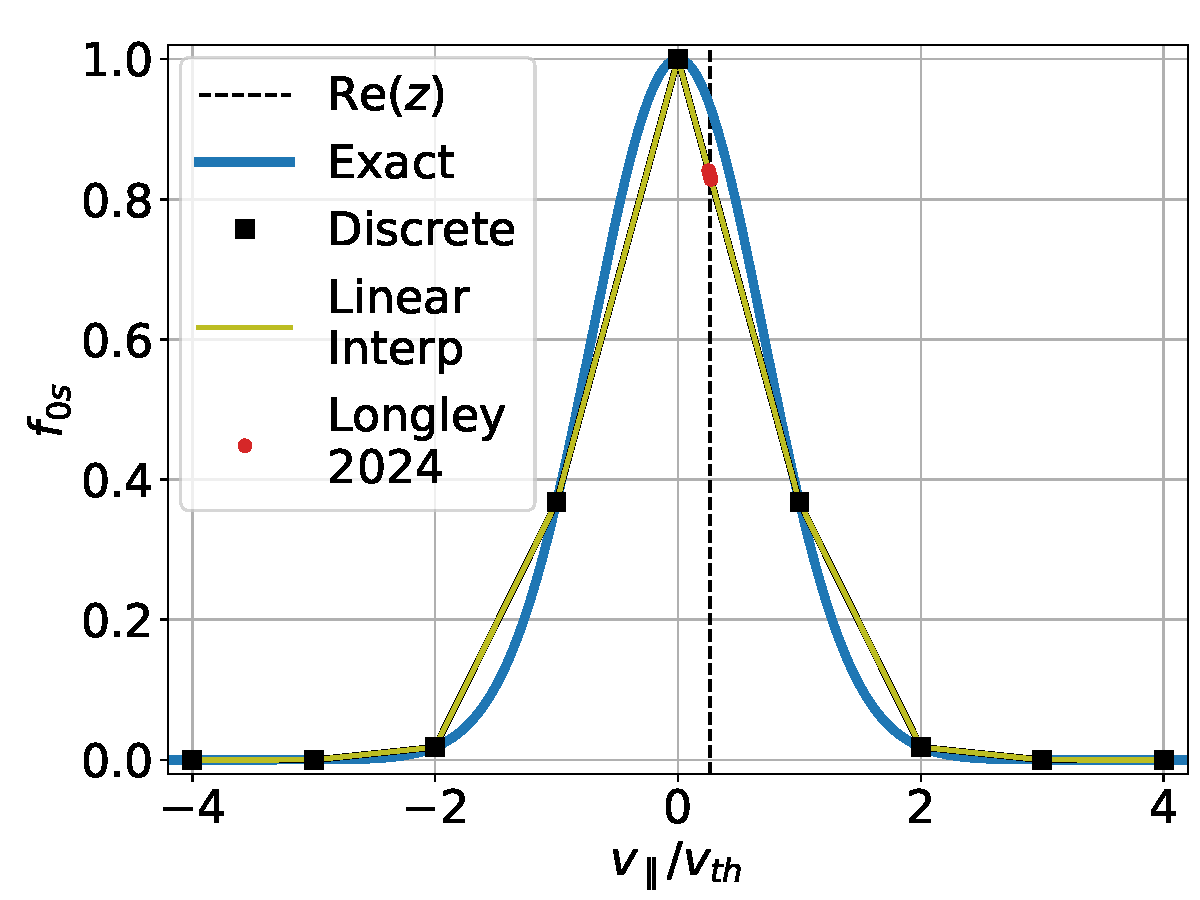
\includegraphics[width=.7\linewidth]{explain.pdf}
	\caption{An example of the representation of a normalized Maxwellian distribution (blue line) with 
	known discrete values (black squares) using either a linear interpolation (green lines)
	or a refined mesh about the pole (red dots) \citep{longley2024}.
	The vertical dashed line represents the real component of the pole, which is defined as $z=\pi/12-10^{-3}i$.}
	\label{f:explainIntegrationMethod}
\end{figure}

Since this method only chooses a finite number of points and can only ever be as good as the interpolation scheme, 
the thought was to instead attempt to get an infinite number of points, i.e., a continuous representation.
Since the adaptive mesh is based on linear interpolation, why not just represent the entire distribution function as a set of linear piecewise functions in the parallel direction, as shown by the orange lines.
For a mesh with $m+1$ points, one will get $m$ elements of the piecewise linear representation.
This results in the distribution function being defined as
\begin{equation}
	f_{0s}(v_\perp,v_\parallel) = 
	\begin{cases}
		f_{0s,0} & v_{\parallel,0} \leq v_\parallel \leq v_{\parallel,1} \\
		f_{0s,1} & v_{\parallel,1} \leq v_\parallel \leq v_{\parallel,2} \\
		\vdots  & \ \\
		f_{0s,j} & v_{\parallel,j} \leq v_\parallel \leq v_{\parallel,j+1} \\
		\vdots & \\
		f_{0s,m} & v_{\parallel,m} \leq v_\parallel \leq v_{\parallel,m+1} 
	\end{cases},
	\label{eq:fLinearFull}
\end{equation}
with
\begin{equation}
	f_{0s,j} (v_\perp, v_\parallel) = a_j(v_\perp) v_\parallel + b_j (v_\perp),
	\label{eq:fLinear}
\end{equation}
where $a_j$ and $b_j$ are polynomial coefficients calculated using
\begin{align}
	a_j(v_\perp) = \frac{f_{0s}(v_\perp, v_{\parallel,j+1}) - f_{0s}(v_\perp, v_{\parallel,j})}{v_{\parallel,j+1}-v_{\parallel,j}}
	\label{eq:aCoeff} \\
	b_j(v_\perp) = f_{0s}(v_\perp, v_{\parallel,j}) - a_j(v_\perp) v_{\parallel,j}.
	\label{eq:bCoeff}
\end{align}
These are just the standard formulas for calculating linear interpolation coeffients. 
Note that the distribution function is an azimuthally symmetric function of $v_\perp$ and $v_\parallel$.
In our case, we only need to do the linear interpolation in the parallel direction.
Therefore, the coefficients $a_j$ and $b_j$ are functions of $v_\perp$.

Thus, any integral regarding $f_{0s}$ can be written as a summation of integrals based on the linear representation in Eq.~\ref{eq:fLinearFull} as
\begin{equation}
	\int_{-\infty}^\infty f_{0s} dv_\parallel = \sum_{j=0}^m \int_{v_{\parallel,j}}^{v_{\parallel,j+1}} f_{0s,j} dv_\parallel.
\end{equation}
With this discrete representation, we can obtain the analytic integrals by substituting Eqs.~\ref{eq:fLinearFull} and \ref{eq:fLinear} into Eqs.~\ref{eq:p1}-\ref{eq:p2} to get
\begin{equation}
	\int_{-\infty}^\infty \frac{f_{0s}(v_\parallel,v_\perp)}{v_\parallel - z} dv_\parallel = 
	\sum_{j=0}^m  \Bigg[ a_j(v_\perp) \big(v_\parallel-z\big) + \big[ a_j(v_\perp) z + b_j(v_\perp) ] \ln \big( v_\parallel - z \big) \Bigg]_{v_{\parallel,j}}^{v_{\parallel,j+1}}
	\label{eq:p1Linear}
\end{equation}
\begin{equation}
	\int_{-\infty}^\infty \frac{f_{0s}(v_\parallel,v_\perp)}{(v_\parallel - z)(v_\parallel - z^*)} dv_\parallel = \sum_{j=0}^m \Bigg[
	- \frac{i \Big( \big[ a_j(v_\perp)z + b_j(v_\perp)\big] \ln \big[ v_\parallel-z \big] - 
		\big[ a_j(v_\perp)z^* + b_j(v_\perp)\big] \ln \big[ v_\parallel-z^* \big] 
		\Big)  }{2 \im(z)} \Bigg]_{v_{\parallel,j}}^{v_{\parallel,j+1}}
	\label{eq:pstarLinear}
\end{equation}
\begin{equation}
	\int_{-\infty}^\infty  \frac{f_{0s,j}(v_\parallel,v_\perp)}{(v_\parallel - z)^2} dv_\parallel = \sum_{j=0}^m \Bigg[
	\frac{-a_j(v_\perp)z - b_j(v_\perp)}{v_\parallel - z} + a_j(v_\perp) \ln\big(v_\parallel-z\big)\Bigg]_{v_{\parallel,j}}^{v_{\parallel,j+1}}
	\label{eq:p2Linear}
\end{equation}
\begin{equation}
	p_1^j (v_\perp, v_\parallel) = \int \frac{f_{0s,j}(v_\parallel,v_\perp)}{v_\parallel - z} dv_\parallel = 
	a_j(v_\perp) \big(v_\parallel-z\big) + \big[ a_j(v_\perp) z + b_j(v_\perp) ] \ln \big( v_\parallel - z \big)
	\label{eq:p1j}
\end{equation}
\begin{equation}
	p_*^j (v_\perp, v_\parallel) =\int \frac{f_{0s,j}(v_\parallel,v_\perp)}{(v_\parallel - z)(v_\parallel - z^*)} dv_\parallel = 
	- \frac{i \Big( \big[ a_j(v_\perp)z + b_j(v_\perp)\big] \ln \big[ v_\parallel-z \big] - 
		\big[ a_j(v_\perp)z^* + b_j(v_\perp)\big] \ln \big[ v_\parallel-z^* \big] 
		\Big)  }{2 \im(z)},
	\label{eq:pstarj}
\end{equation}
\begin{equation}
	p_2^j (v_\perp, v_\parallel) =\int \frac{f_{0s,j}(v_\parallel,v_\perp)}{(v_\parallel - z)^2} dv_\parallel = 
	\frac{-a_j(v_\perp)z - b_j(v_\perp)}{v_\parallel - z} + a_j(v_\perp) \ln\big(v_\parallel-z\big)
	\label{eq:p2j}
\end{equation}
where $p_1^j(v_\perp)$, $p_*^j(v_\perp)$, and $p_2^j(v_\perp)$ are the indefinite integrals corresponding to 
Eqs.~\ref{eq:p1}-\ref{eq:p2}, respectively, for element $j$.
We can obtain the full integration from $-\infty$ to $\infty$ (which is realistically $-v_{\parallel,\max}$ to $v_{\parallel,\max}$)
\begin{equation}
	p(v_\perp) = \sum_j p^j(v_\perp, v_{\parallel,j+1}) - p^j(v_\perp, v_{\parallel,j}),
	\label{eq:finalPoleIntegral}
\end{equation}
where $p$ is a placeholder for the specific pole integral being carried out from Eqs.~\ref{eq:p1j} to \ref{eq:p2j}.

% Maybe we say somewhere that the second order pole is the most difficult to get right because of it being an even function about the pole (no terms to cancel).

We will test this pole integration method with the normalized Maxwellian distribution function from Eq.~\ref{eq:norm_maxwellian} with the known exact solutions from Eqs.~\ref{eq:p1Exact}-\ref{eq:p2Exact}.
The pole is chosen to be at $z=\pi/12 - i \gamma$ where $\gamma=(\nu/k_\parallel)/v_{th}$ (see Eq.~\ref{eq:z}) is varied logarithmically from $10^{-6}$ to $10^{0}$.
Note that the real part of $z$ is chosen specifically to be irrational such that it will always be in between the discrete points. 
This provides the best case scenario for our method.

Figs.~\ref{f:poleIntegrateError0}-\ref{f:poleIntegrateError-5} show how the linear pole integration from Eq.~\ref{eq:finalPoleIntegral} (red x's) compares with the exact solution from Eqs.~\ref{eq:p1Exact}-\ref{eq:p2Exact} (black line), a simple trapezoidal integration (orange dots), and the pole refinement technique \citep{longley2024} (blue circles) for varying discrete velocity mesh resolutions varying from $\Delta v_\parallel/v_{th}=10^0$ to $\Delta v_\parallel/v_{th}=10^{-5}$.
We show the real (top) and imaginary (bottom) solutions for each of the three poles from Eqs.~\ref{eq:p1}-\ref{eq:p2}.
The $x$-axis of all of these plots is $\gamma$. 
Since the real part of the pole is constant at 0.25, the $\gamma$ can be seen as the distance of the pole from the real axis.
As $\gamma$ approaches $\infty$, or as we move to the right in Figs.~\ref{f:poleIntegrateError0}-\ref{f:poleIntegrateError-5}, the pole moves further away from the real axis.
The further the pole is from the real axis, the less it impacts the final integration result resulting in an easier calculation.
As $\gamma$ approaches 0, or as we move to the left in Figs.~\ref{f:poleIntegrateError0}-\ref{f:poleIntegrateError-5}, the pole approaches the real axis.
The closer the pole is to the real axis, the more difficult the calculations are.
Therefore, the solutions for all of the integration methods are expected to be more correct towards the right and have more error towards the left.

Fig.~\ref{f:poleIntegrateError0} has the coarsest mesh and presents why this linear interpolation method is so powerful.
The velocity mesh and the discrete distribution function correspond exactly to the example in Fig.~\ref{f:explainIntegrationMethod}.
As would be expected for representing a Maxwellian distribution using only 9 points, trapezoidal is only correct toward the right where the pole is far from the real axis.
The pole refined integration technique is an improvement and is generally more correct for more values of $\gamma$.
The linear interpolation integration method shows significant improvement over all of the other methods and provides generally correct asymptotic behavor as $\gamma$ approaches 0 that the other methods do not.
Thus, for even a very coarse mesh of only 9 points, our technique is significantly better than previously used methods.


A very nice result for all of the methods is that the imaginary component of the double pole at $z$ and $z^*$ (Eq.~\ref{eq:pstar}) should be exactly 0 (Eq.~\ref{eq:pstarExact}).
Every integration method captures this behavior.
% Dunno what else to say here, but, just wanted to explicitly point this out somewhere


As we increase the mesh resolution to have $\Delta v_\parallel/v_{th}=10^{-1}$, each of the methods generally improve.
This will be the case for each increase in resolution.
The pole refined, linear interpolation, and trapezoidal methods fully capture the real part of the first order pole. 
The linear interpolation method fully captures the real part of the double pole and the imaginary part of the second order pole.
Furthermore, the linear interpolation method almost exactly captures the real part of the second order pole.


At a resolution of $\Delta v_\parallel/v_{th}=10^{-2}$, the linear interpolation appears to fully capture the real part of the second order pole.
At this resolution, the linear interpolation method has now fully captured all of the calculations. 
Note that in testing this for the full spectrum calculations, we found that $\Delta v_\parallel/v_{th}=10^{-2.3}$ provided sufficient parallel velocity resolution to reach a converged solution. 
This will likely have to modified depending on the structure of the distribution function.

The other methods just provide general improvements for this increased resolution. 
This is the case for $\Delta v_\parallel/v_{th}=10^{-3}$ as well.
At $\Delta v_\parallel/v_{th}=10^{-4}$, the pole refined method fully captures everything but the real part of the second order pole.
Even at the finest resolution tested at $\Delta v_\parallel/v_{th}=10^{-5}$, the real part of the second order pole is never fully captured.
Interestingly, the trapezoidal integration at this resolution actually provides better results than the pole refined method for certain $\gamma$ (which also happen to be around realistic ionospheric and radar values).
Nonetheless, Figs.~\ref{f:poleIntegrateError0}-\ref{f:poleIntegrateError-5} show the superiority of the linear interpolation method versus the other methods.

% I should add Gaussian quadrature as another integration method here?
\begin{figure}[!htb]
	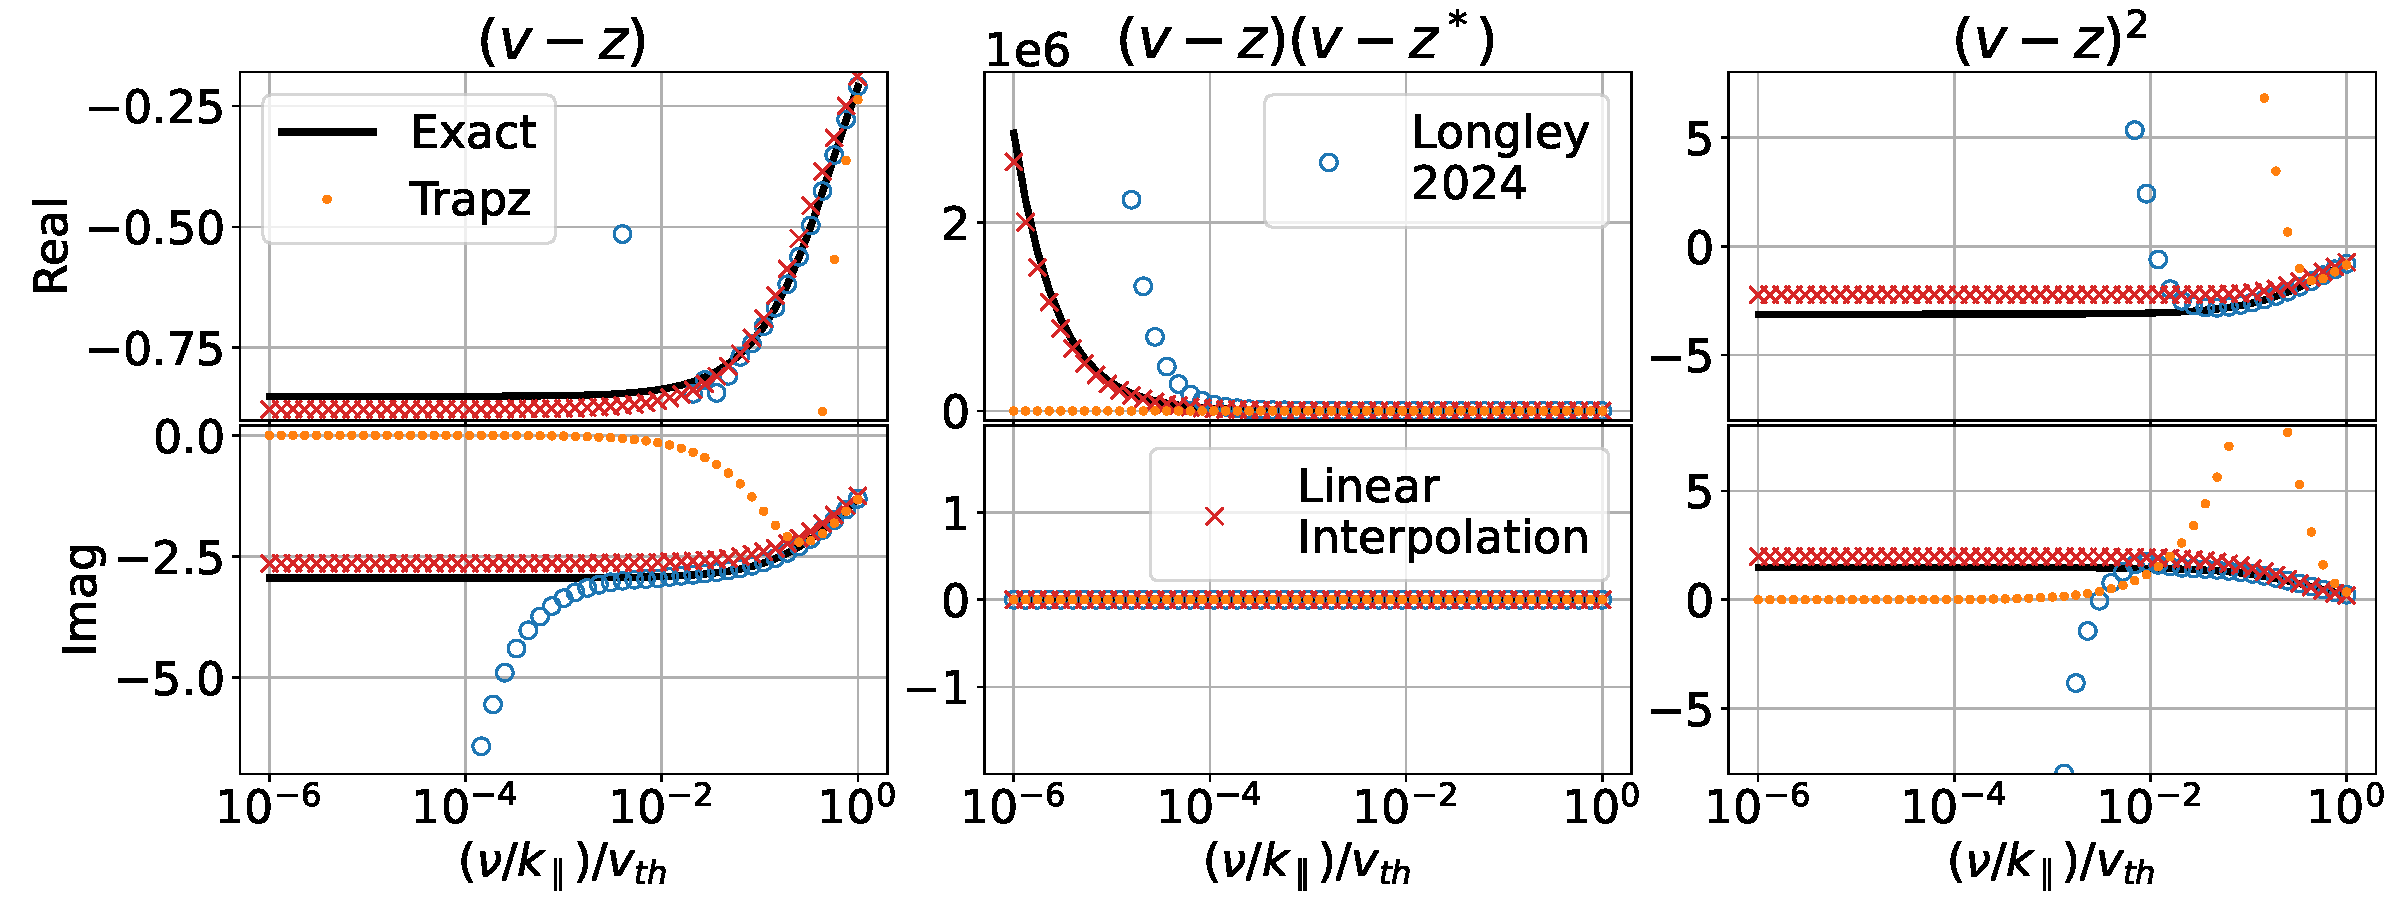
\includegraphics[width=\linewidth]{poleIntegrate_error_0.pdf}
	\caption{Comparison of error between exact solution from Eqs.~\ref{eq:p1Exact}-\ref{eq:p2Exact} (black line),
		trapezoidal integration (orange dots),
		pole refined method from \cite{longley2024} (blue circles),
		and our linear interpolation method from Eqs.~\ref{eq:finalPoleIntegral} (red x's).
		Each column corresponds to the solution for a different pole (Eqs.~\ref{eq:p1}-\ref{eq:p2}, respectively)
		with the real and imaginary parts on the top and bottom panels, respectively.
		The pole is $z=\pi/12-i\gamma$.
		The original mesh resolution is $\Delta v_\parallel/v_{th}=10^0$.}
	\label{f:poleIntegrateError0}
\end{figure}

\begin{figure}[!htb]
	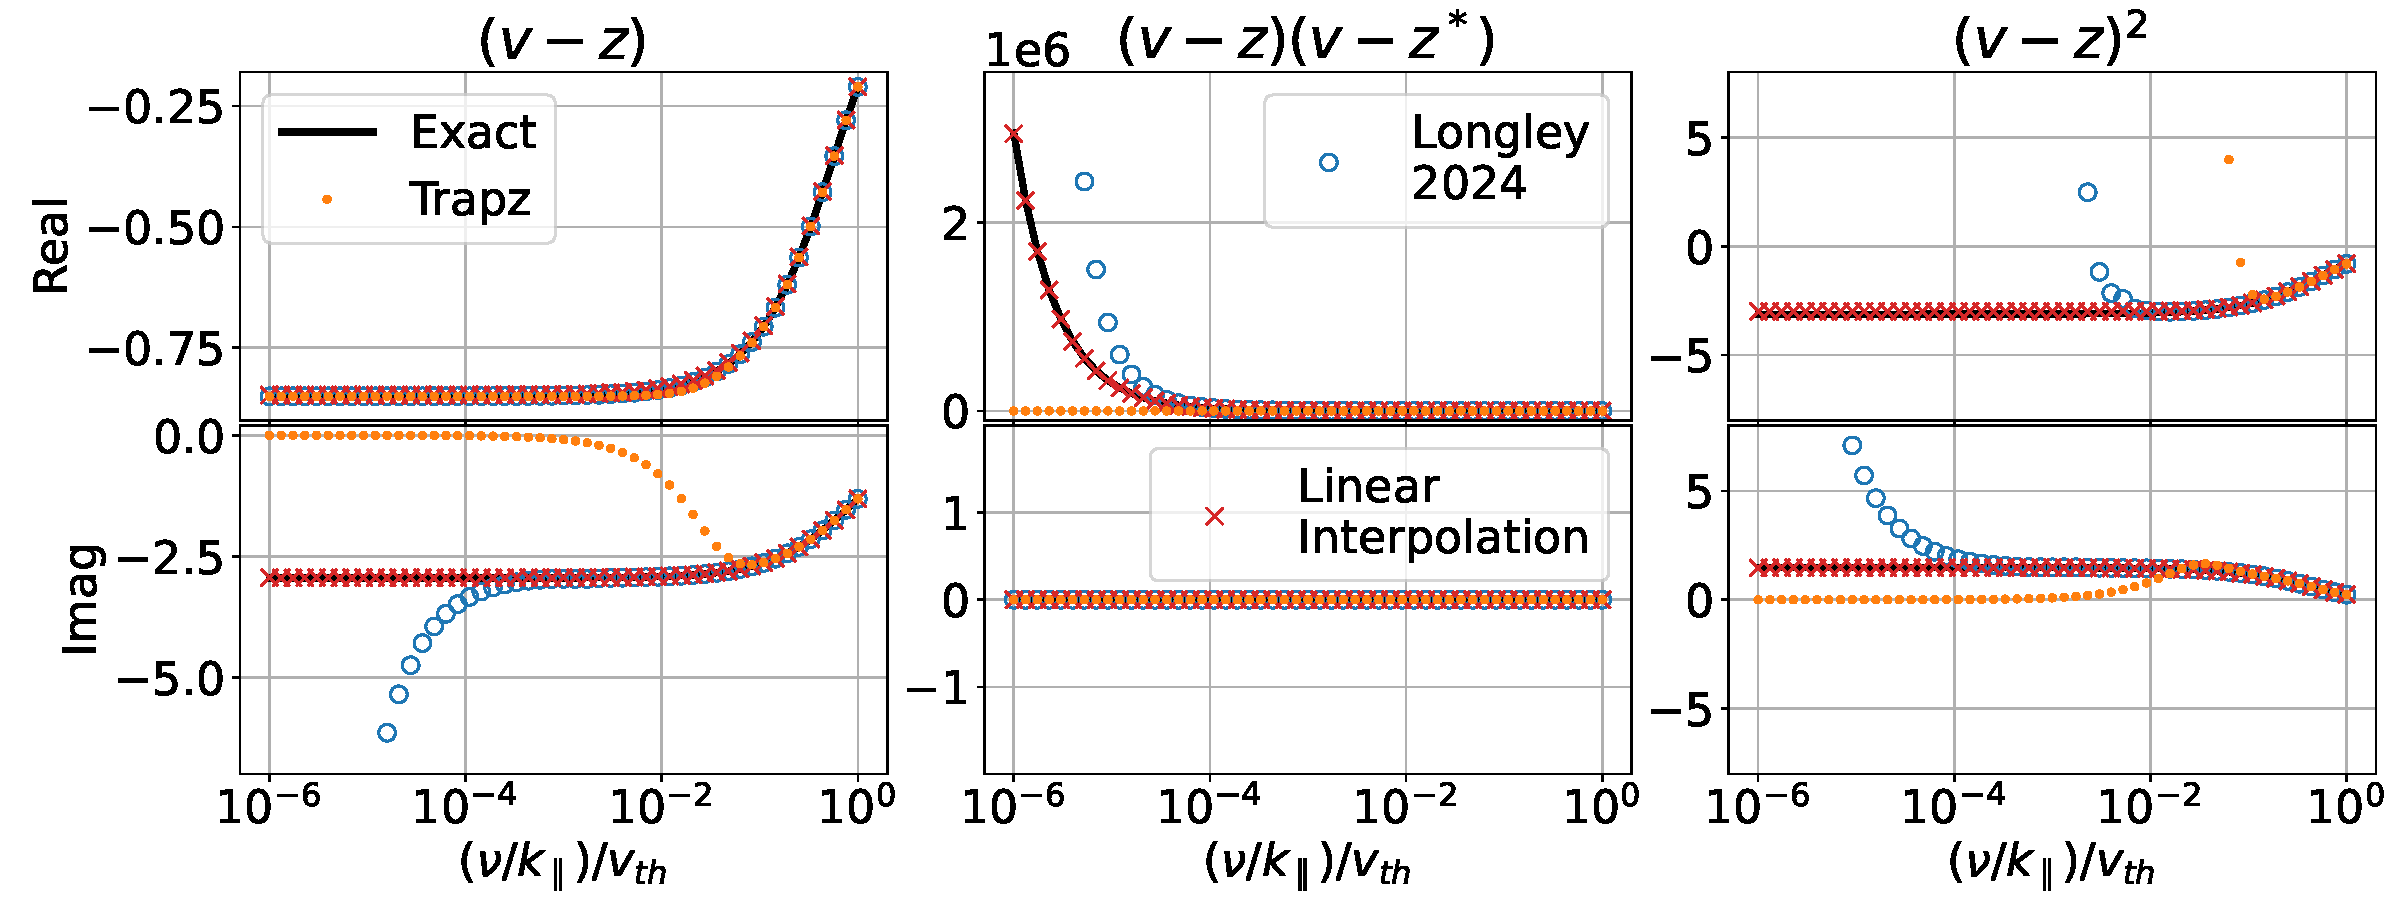
\includegraphics[width=\linewidth]{poleIntegrate_error_-1.pdf}
	\caption{Same as Fig.~\ref{f:poleIntegrateError0} but with $\Delta v_\parallel/v_{th}=10^{-1}$.}
	\label{f:poleIntegrateError-1}
\end{figure}

\begin{figure}[!htb]
	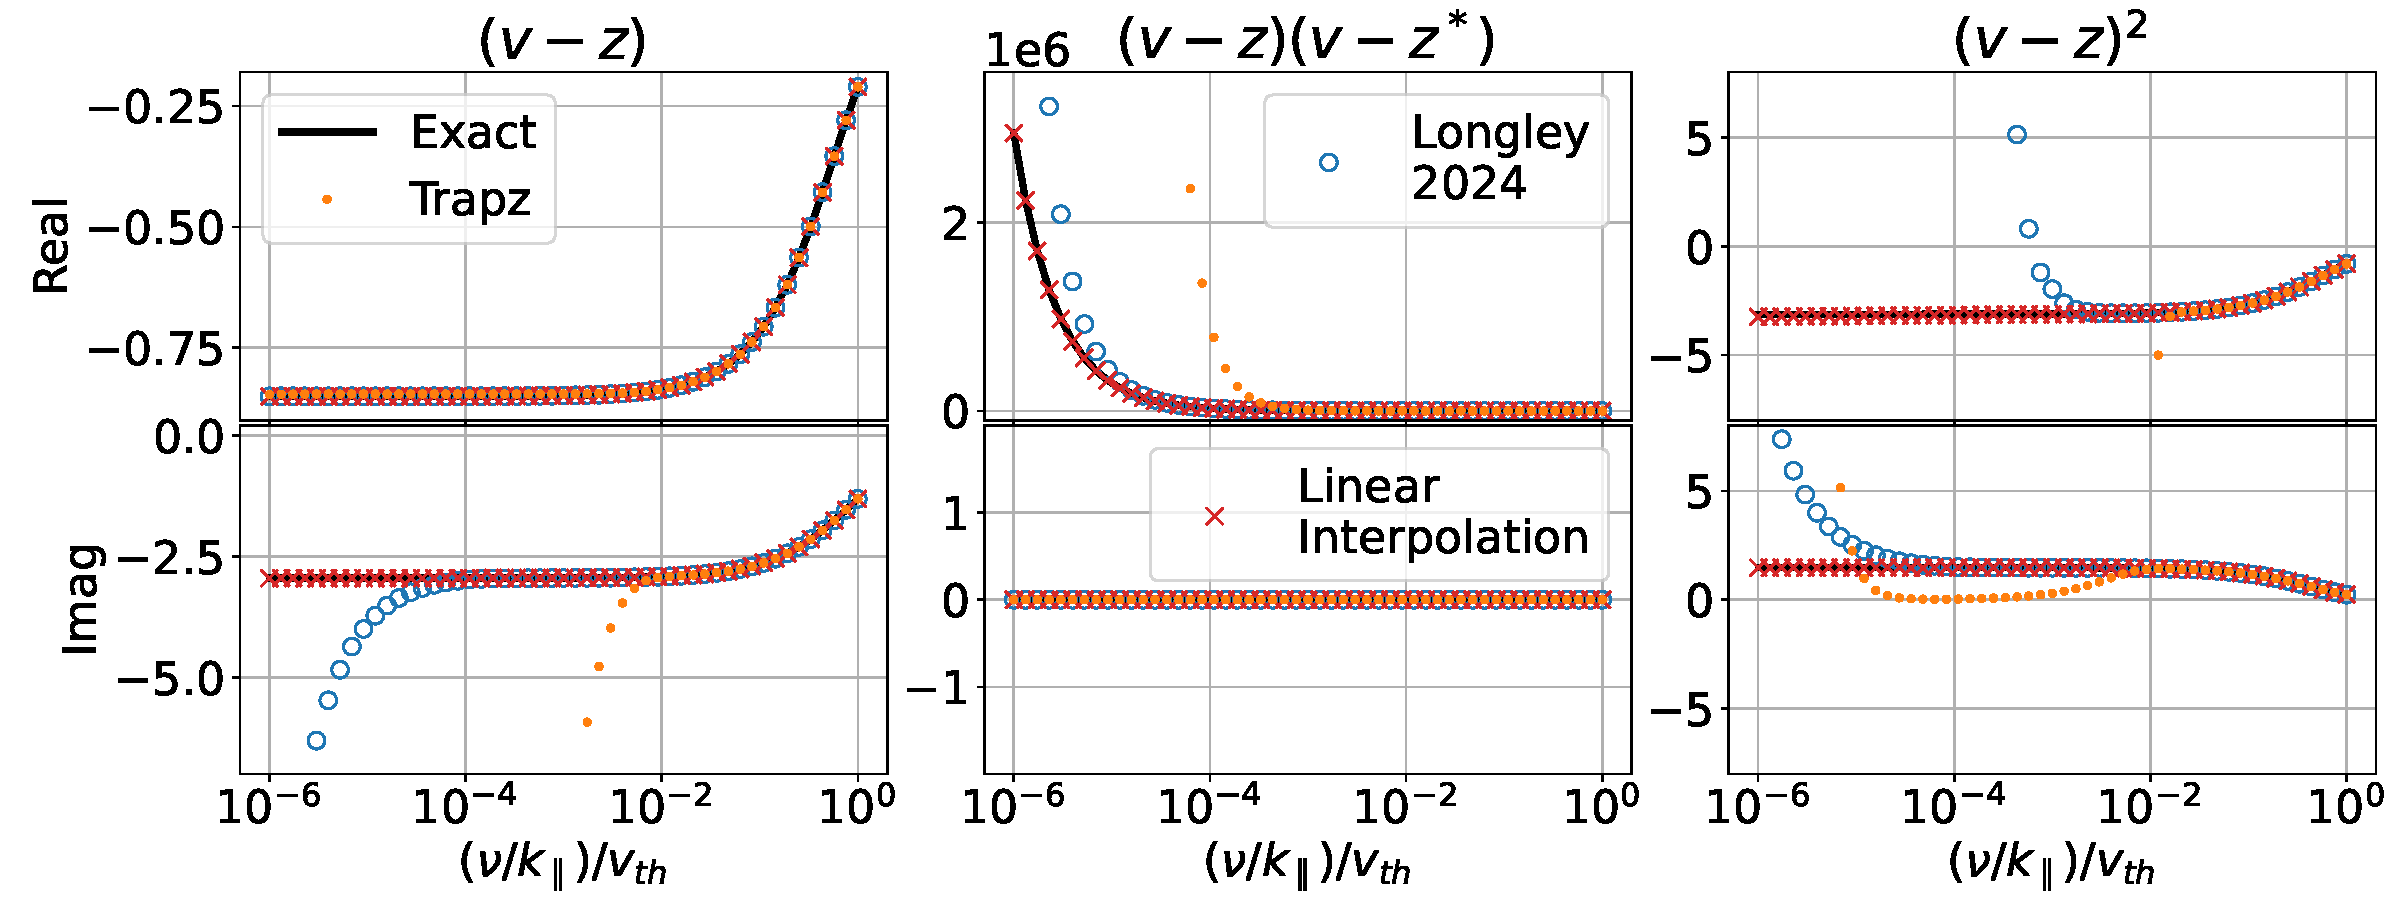
\includegraphics[width=\linewidth]{poleIntegrate_error_-2.pdf}
	\caption{Same as Fig.~\ref{f:poleIntegrateError0} but with $\Delta v_\parallel/v_{th}=10^{-2}$.}
	\label{f:poleIntegrateError-2}
\end{figure}

\begin{figure}[!htb]
	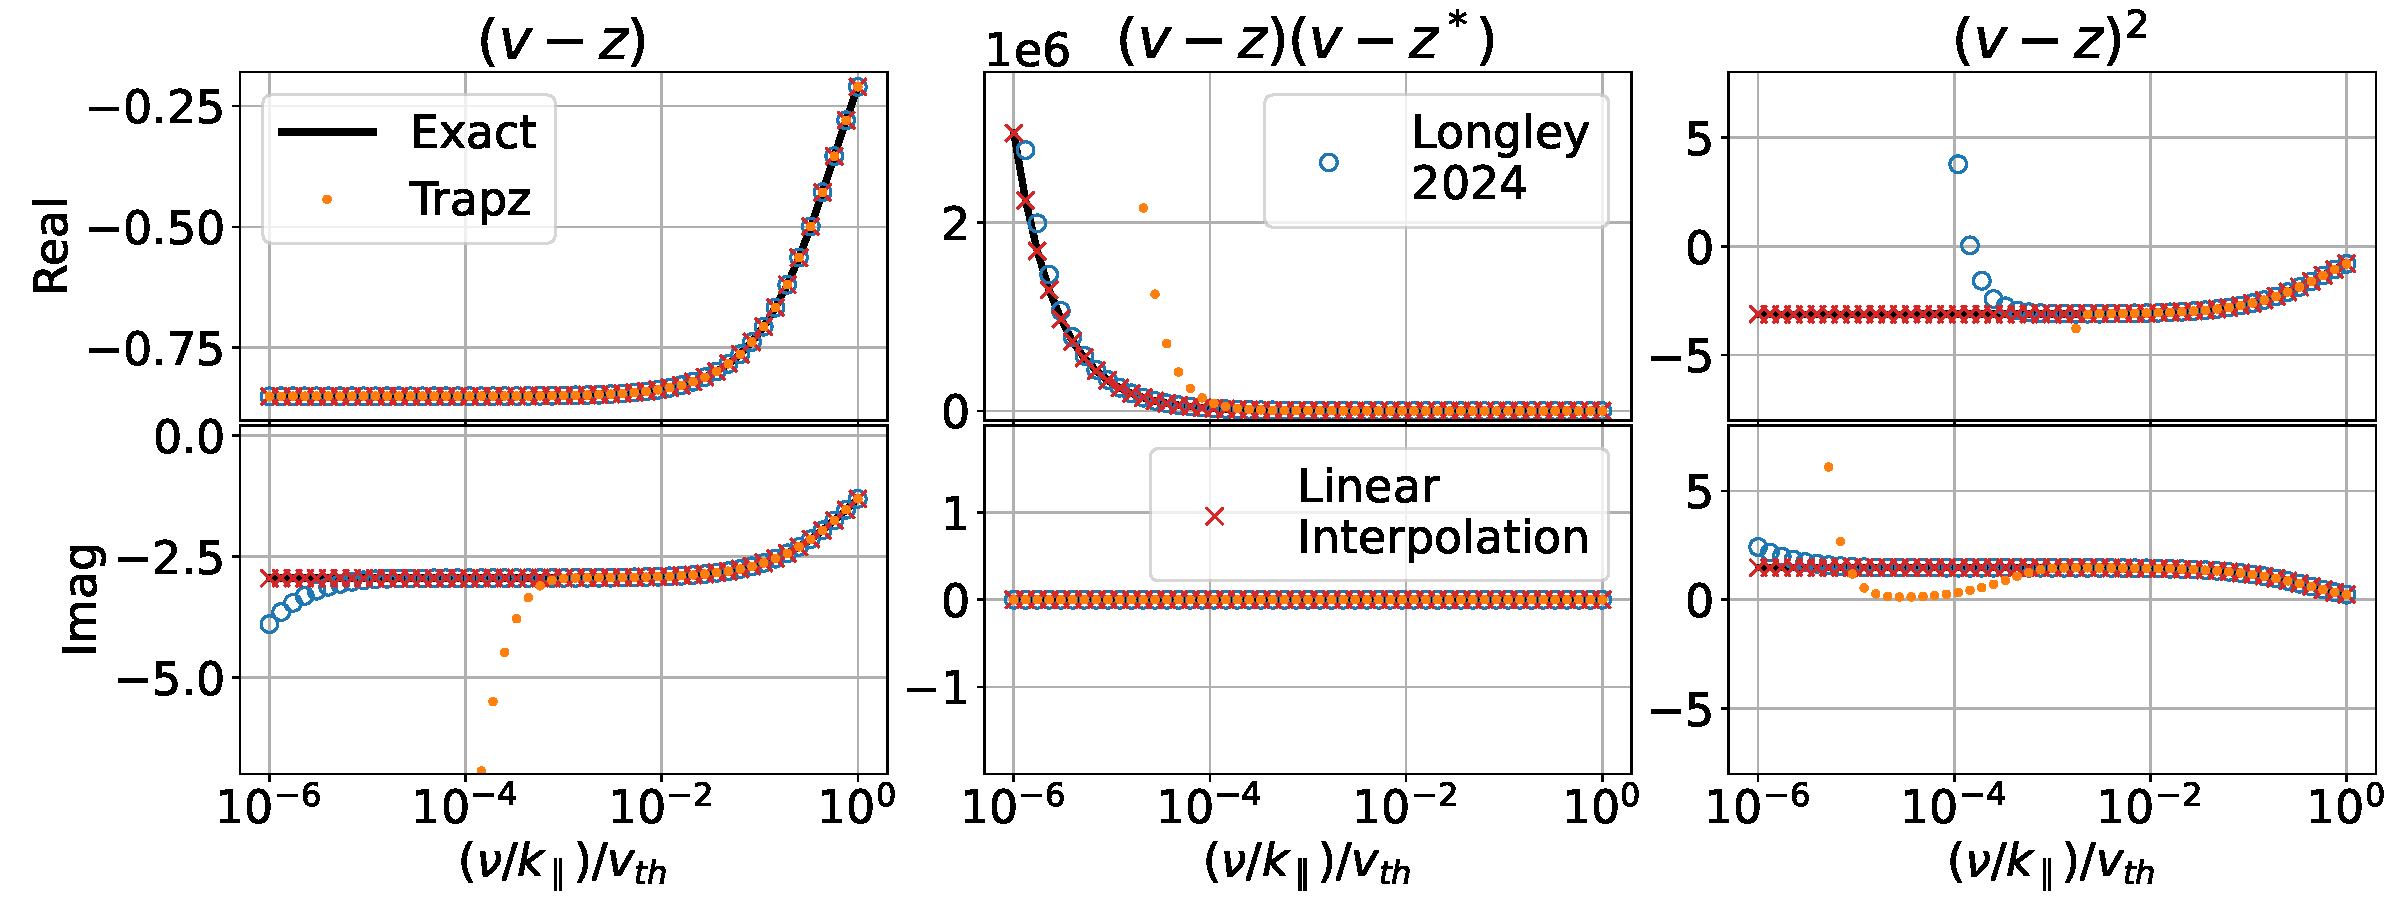
\includegraphics[width=\linewidth]{poleIntegrate_error_-3.pdf}
	\caption{Same as Fig.~\ref{f:poleIntegrateError0} but with $\Delta v_\parallel/v_{th}=10^{-3}$.}
	\label{f:poleIntegrateError-3}
\end{figure}

\begin{figure}[!htb]
	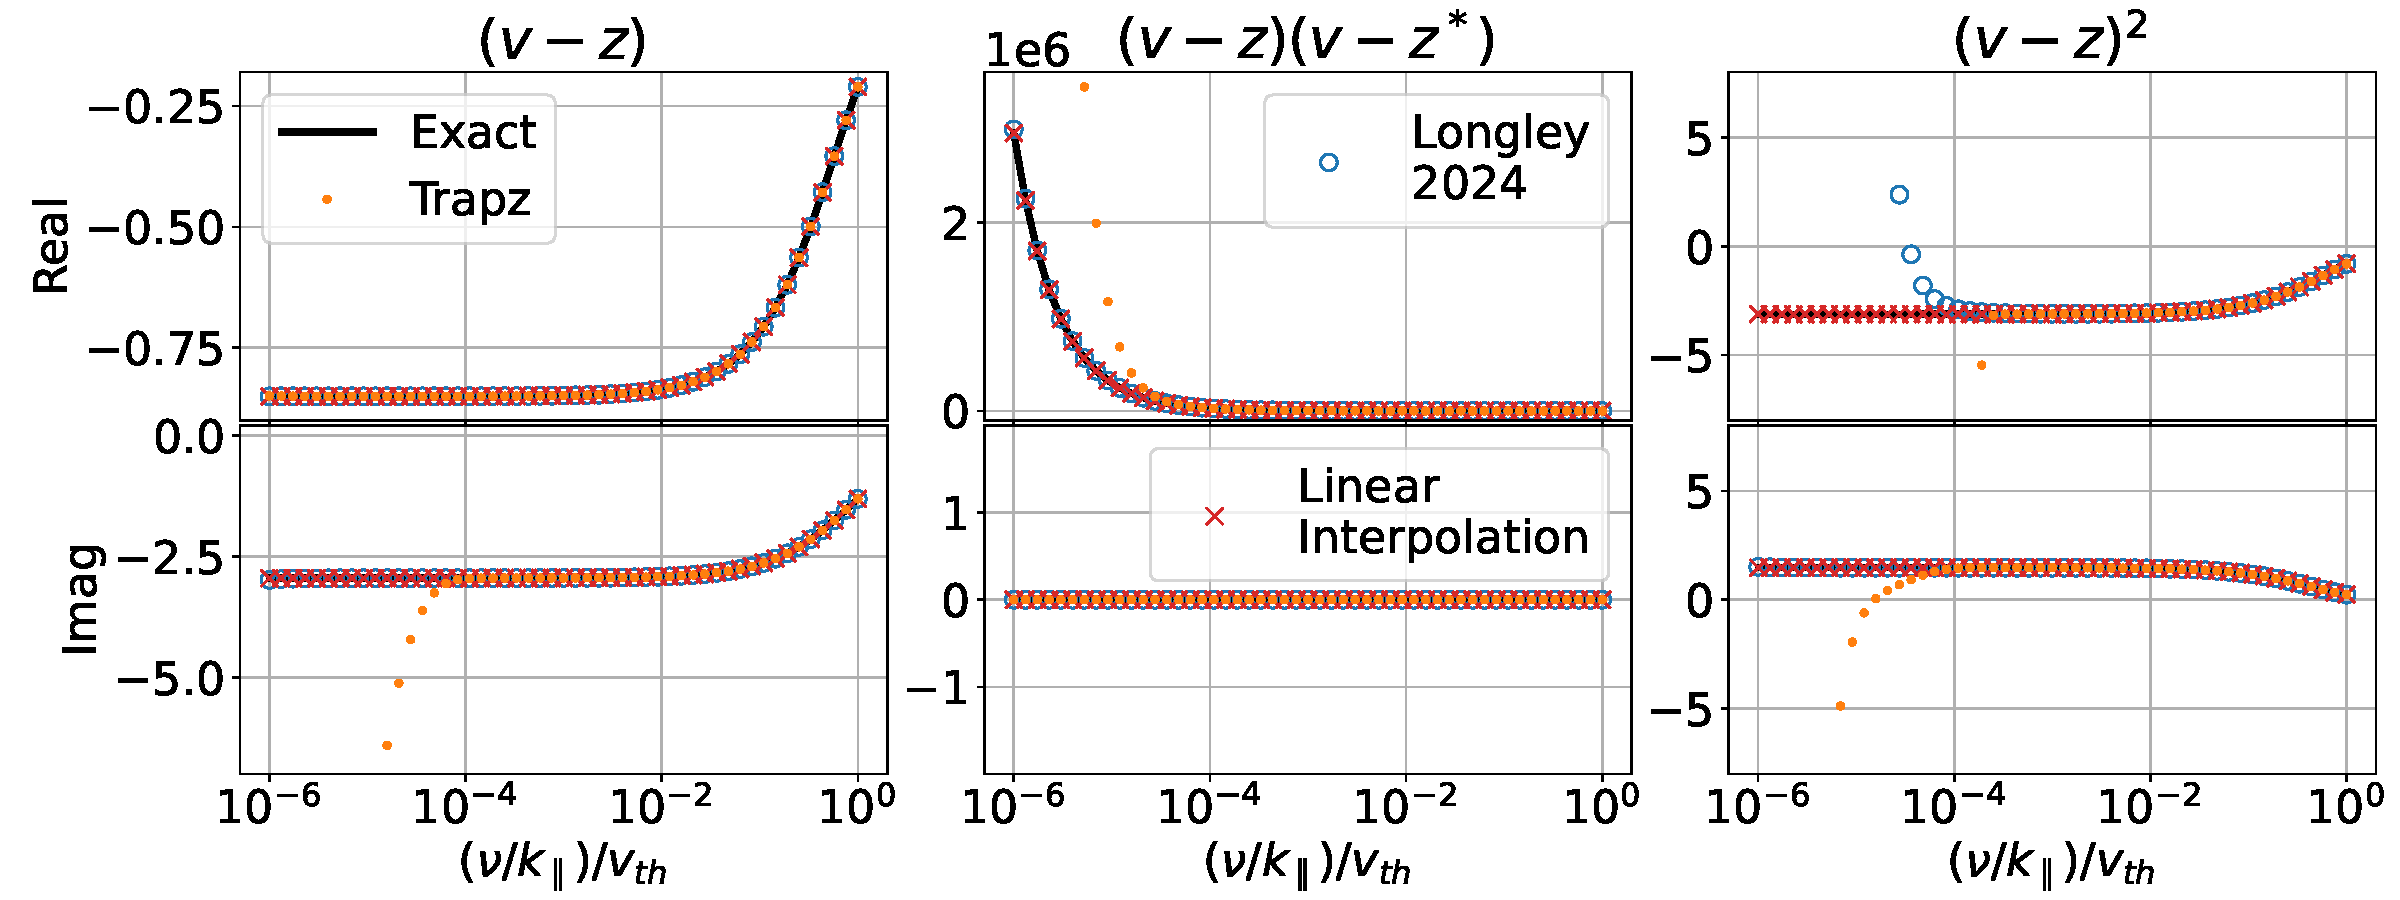
\includegraphics[width=\linewidth]{poleIntegrate_error_-4.pdf}
	\caption{Same as Fig.~\ref{f:poleIntegrateError0} but with $\Delta v_\parallel/v_{th}=10^{-4}$.}
	\label{f:poleIntegrateError-4}
\end{figure}

\begin{figure}[!htb]
	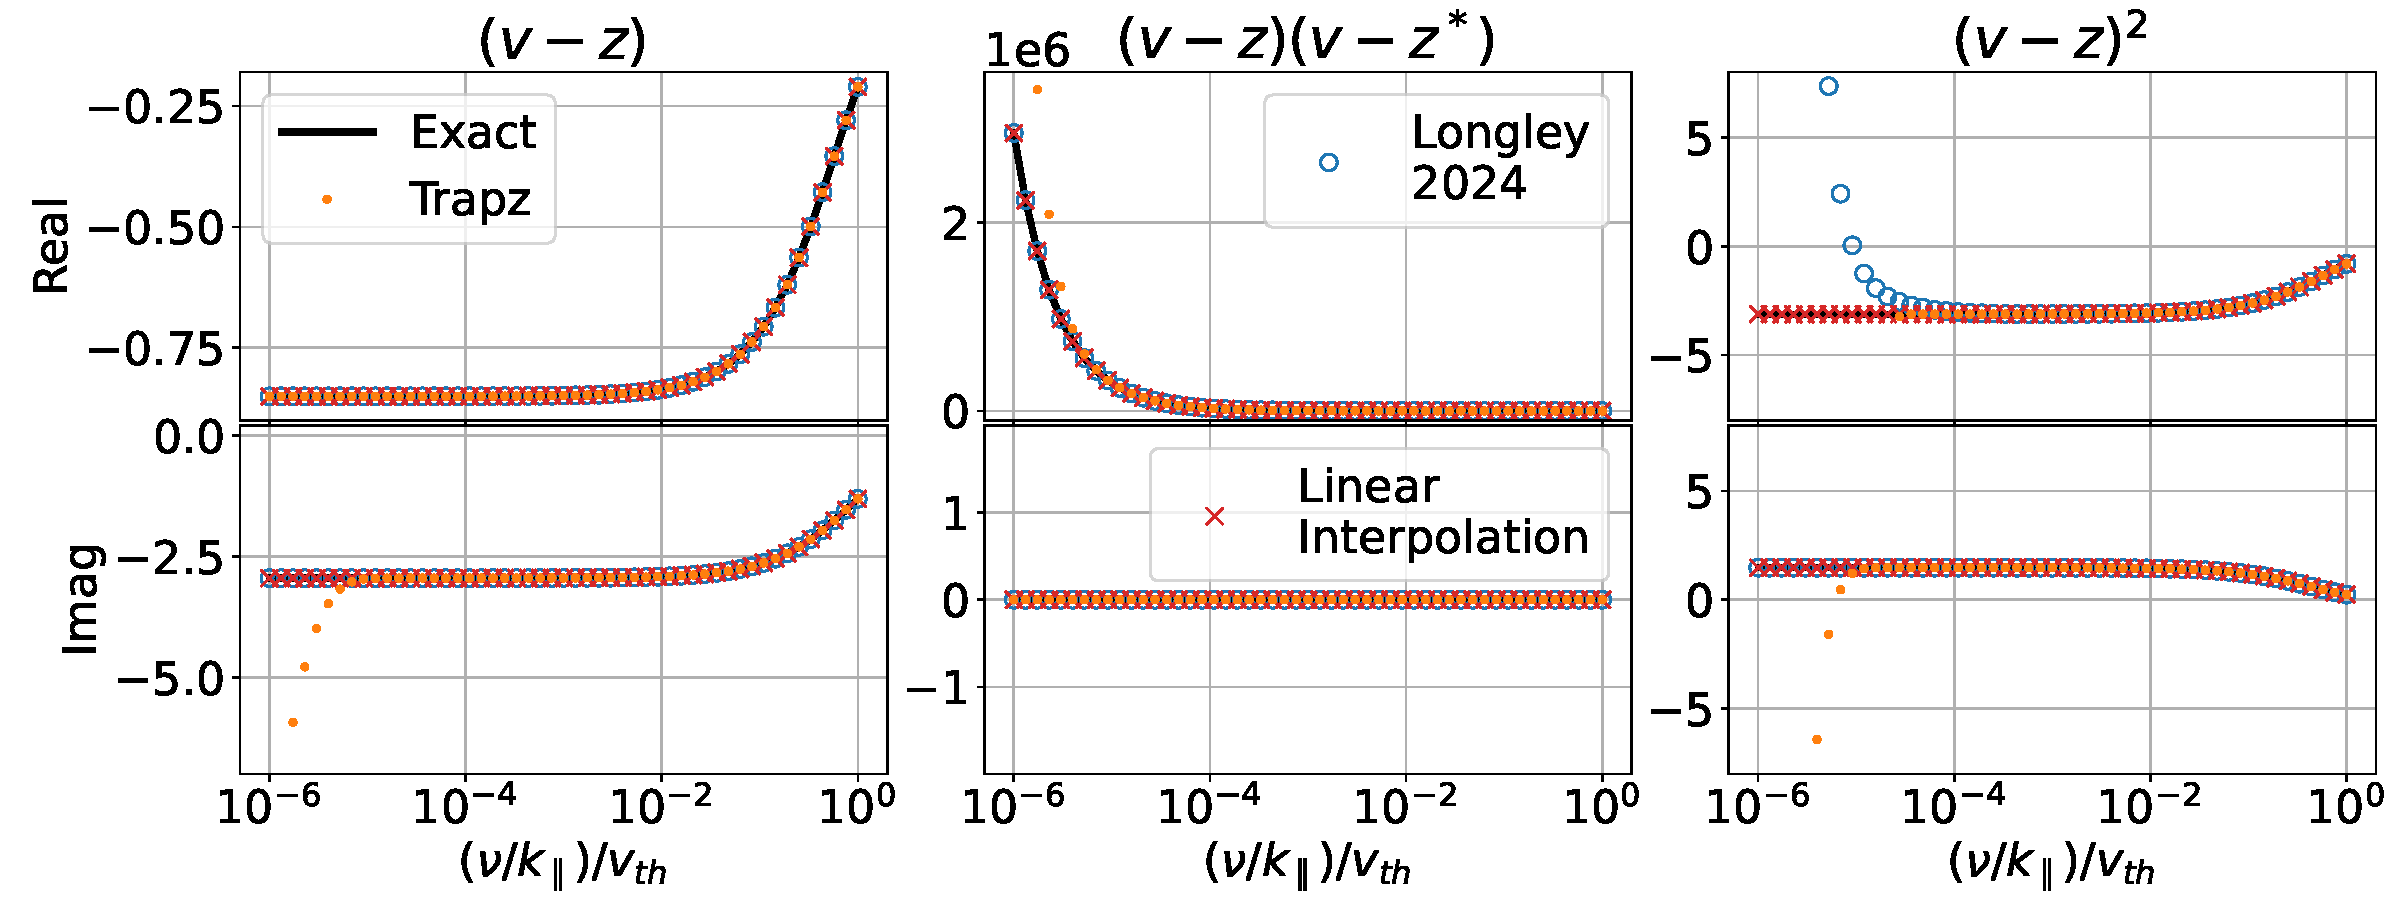
\includegraphics[width=\linewidth]{poleIntegrate_error_-5.pdf}
	\caption{Same as Fig.~\ref{f:poleIntegrateError0} but with $\Delta v_\parallel/v_{th}=10^{-5}$.}
	\label{f:poleIntegrateError-5}
\end{figure}

Now, these are for the best case scenario where the real part of the pole is not in between the discrete points.
In the case where the real part is exactly on a discrete value, what would this look like? 
Figs.~\ref{f:poleIntegrateError0_pole0}-\ref{f:poleIntegrateError-5_pole0} show the same general type of plots as Figs.~\ref{f:poleIntegrateError0}-\ref{f:poleIntegrateError-5} but with the pole at $z=0-i\gamma$.
This will ensure that for every possible resolution, the pole will coincide with a point on the discrete velocity mesh.
We find the same general trends as in the Figs.~\ref{f:poleIntegrateError0}-\ref{f:poleIntegrateError-5}.
The only difference is that our linear interpolation method requires a resolution of $\Delta v_\parallel/v_{th}=10^{-3}$ to converge to the exact solution.
This is likely one of the reasons it requires a mesh of $\Delta v_\parallel/v_{th}=10^{-2.3}$ to reach convergence for the full spectrum calculation.


\begin{figure}[!htb]
	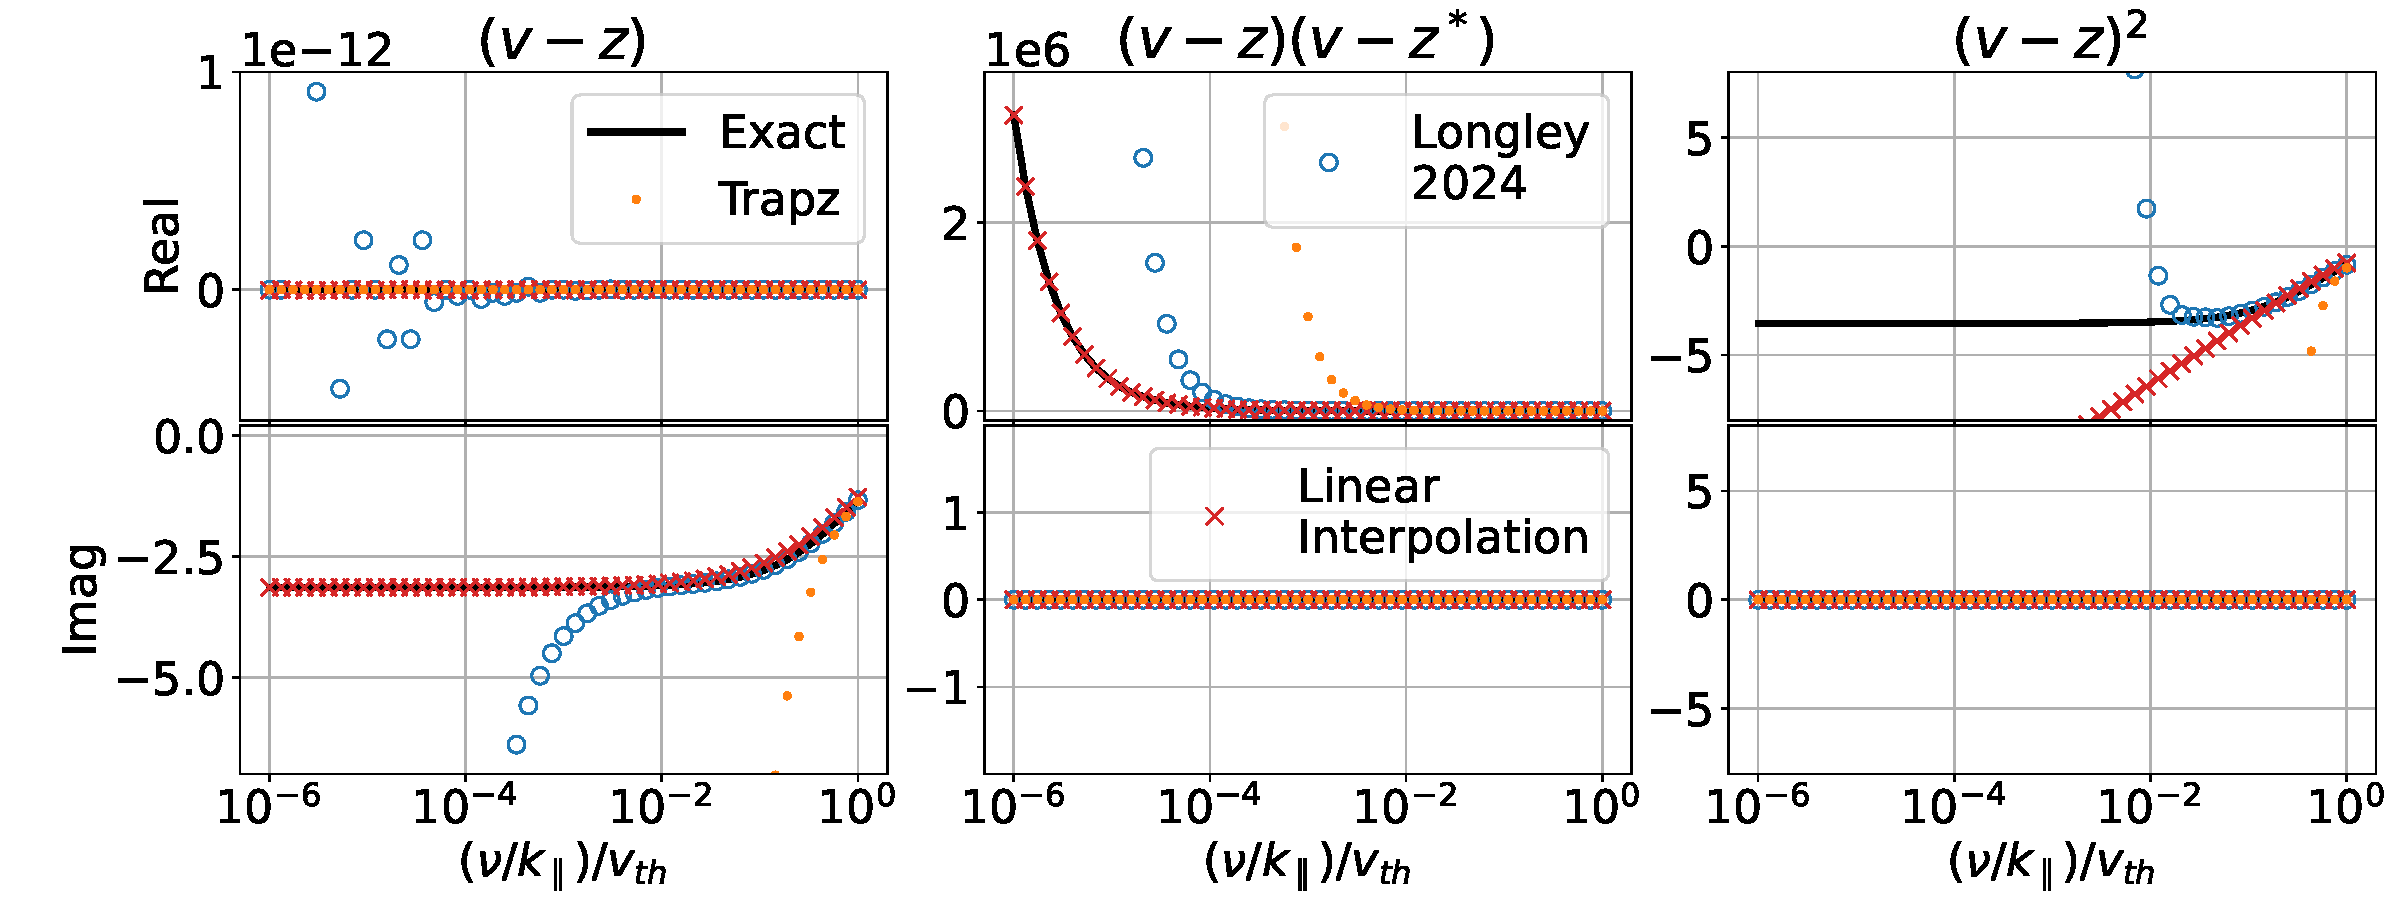
\includegraphics[width=\linewidth]{poleIntegrate_error_pole0_0.pdf}
	\caption{Comparison of error between exact solution from Eqs.~\ref{eq:p1Exact}-\ref{eq:p2Exact} (black line),
		trapezoidal integration (orange dots),
		pole refined method from \cite{longley2024} (blue circles),
		and our linear interpolation method from Eqs.~\ref{eq:finalPoleIntegral} (red x's).
		Each column corresponds to the solution for a different pole (Eqs.~\ref{eq:p1}-\ref{eq:p2}, respectively)
		with the real and imaginary parts on the top and bottom panels, respectively.
		The pole is $z=\pi/12-i\gamma$.
		The original mesh resolution is $\Delta v_\parallel/v_{th}=10^0$.}
	\label{f:poleIntegrateError0_pole0}
\end{figure}

\begin{figure}[!htb]
	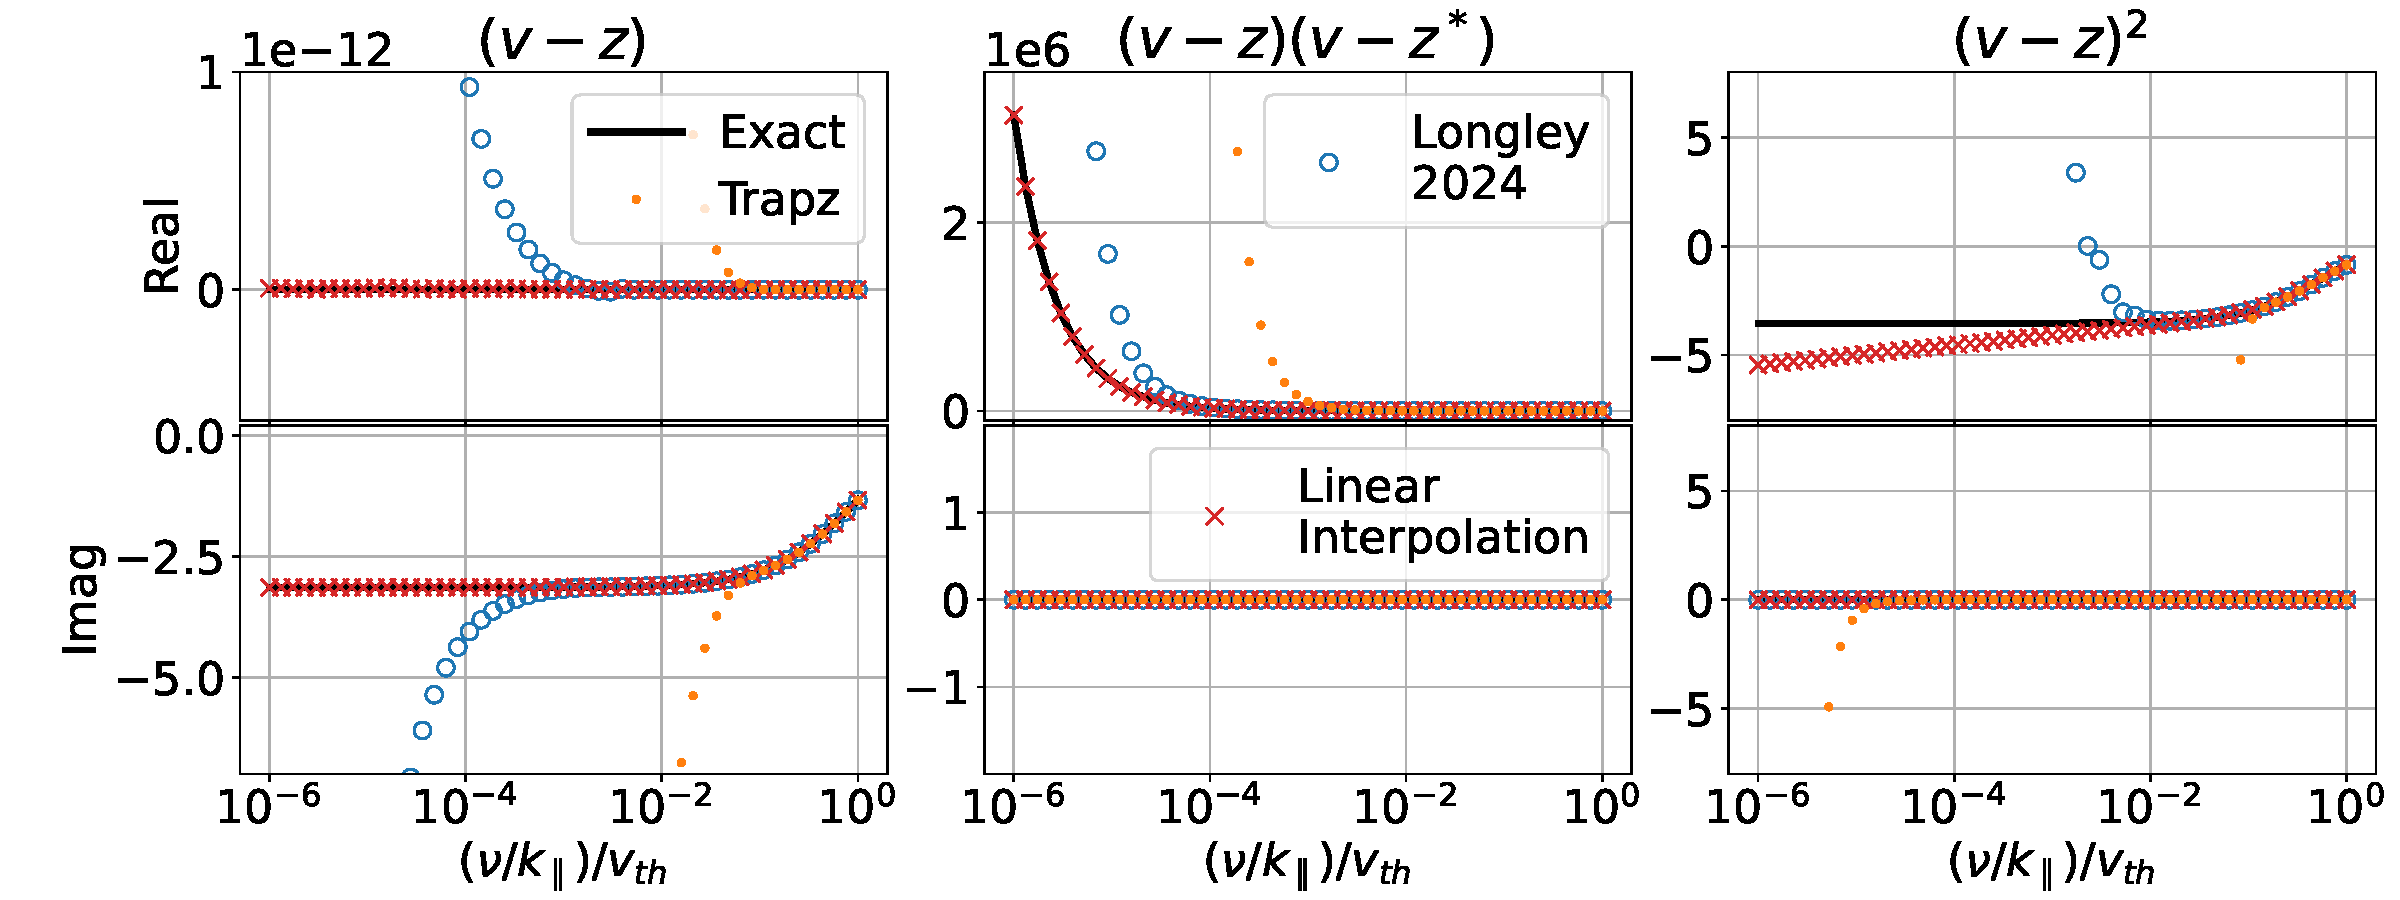
\includegraphics[width=\linewidth]{poleIntegrate_error_pole0_-1.pdf}
	\caption{Same as Fig.~\ref{f:poleIntegrateError0_pole0} but with $\Delta v_\parallel/v_{th}=10^{-1}$.}
	\label{f:poleIntegrateError-1_pole0}
\end{figure}

\begin{figure}[!htb]
	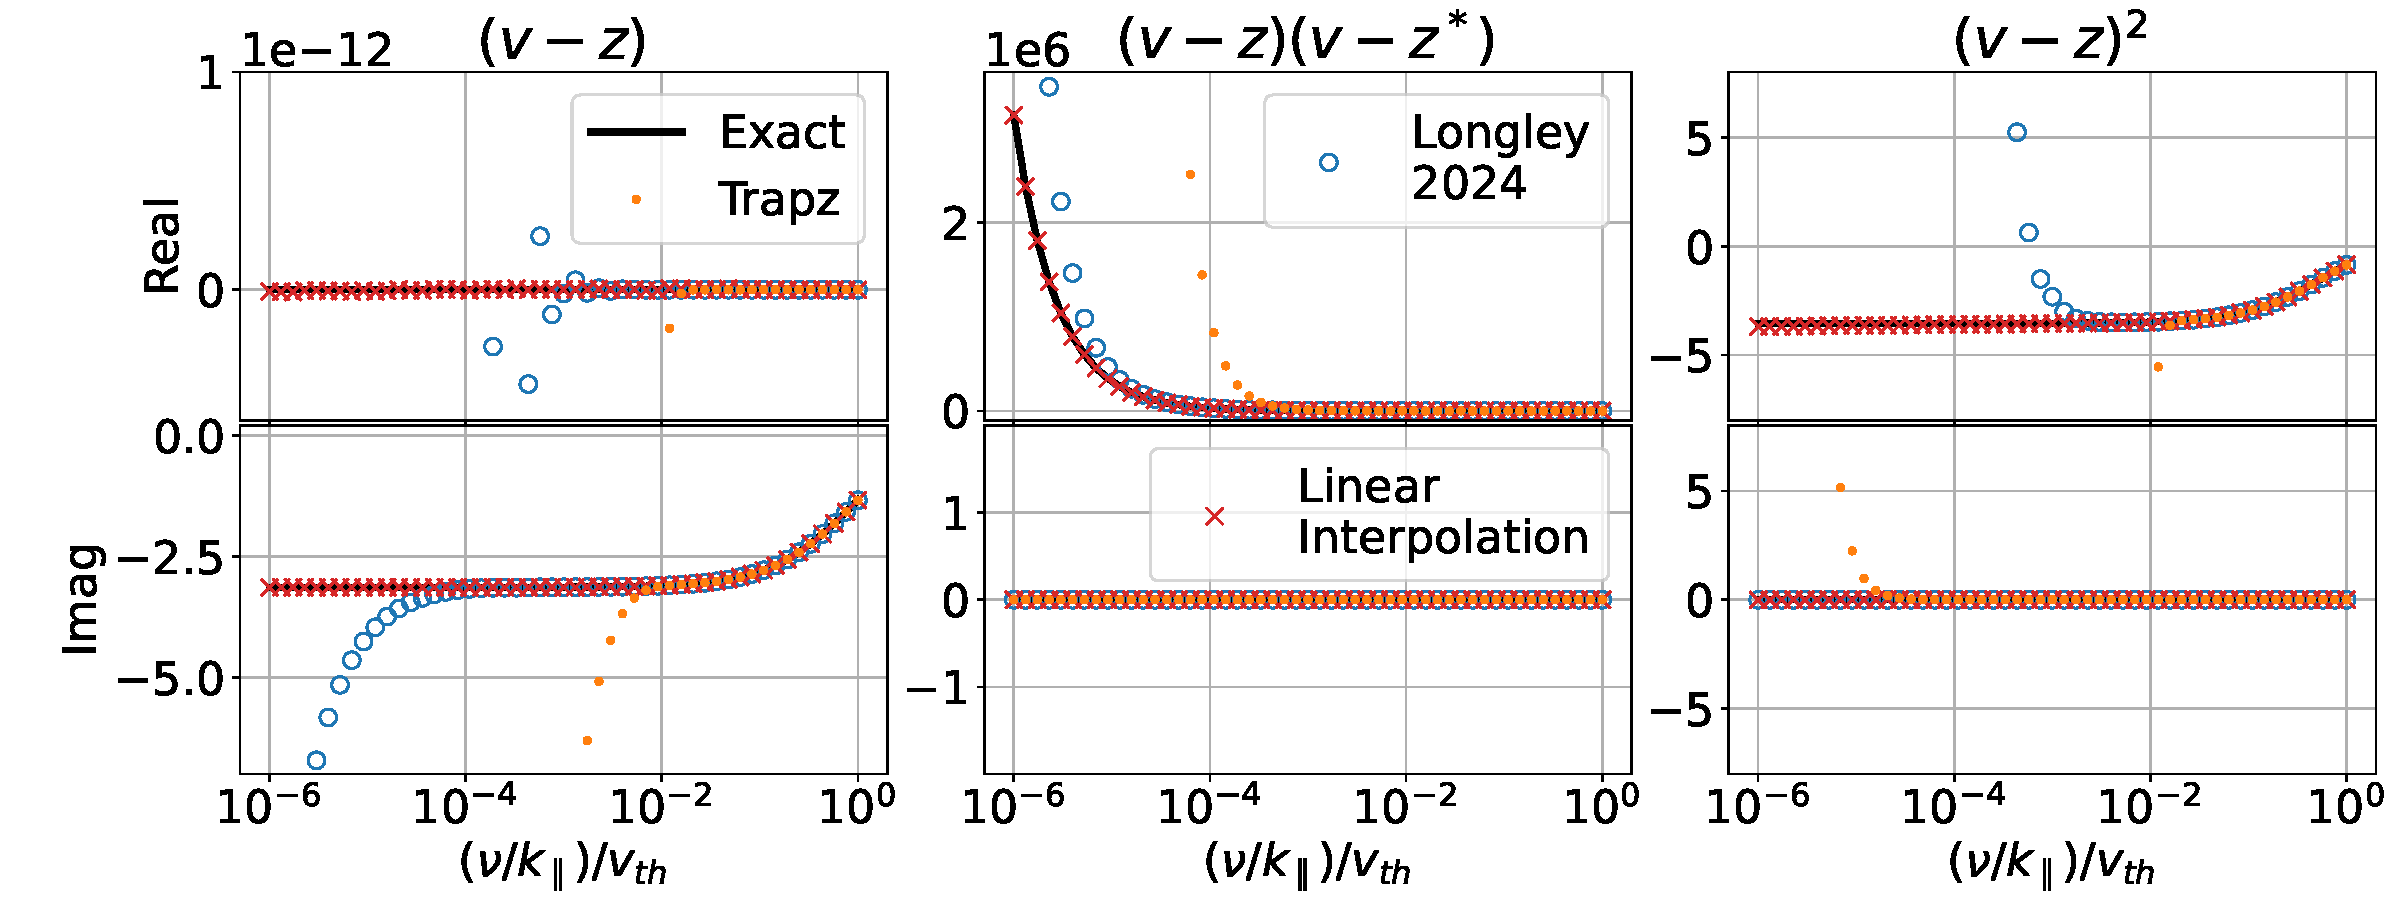
\includegraphics[width=\linewidth]{poleIntegrate_error_pole0_-2.pdf}
	\caption{Same as Fig.~\ref{f:poleIntegrateError0_pole0} but with $\Delta v_\parallel/v_{th}=10^{-2}$.}
	\label{f:poleIntegrateError-2_pole0}
\end{figure}

\begin{figure}[!htb]
	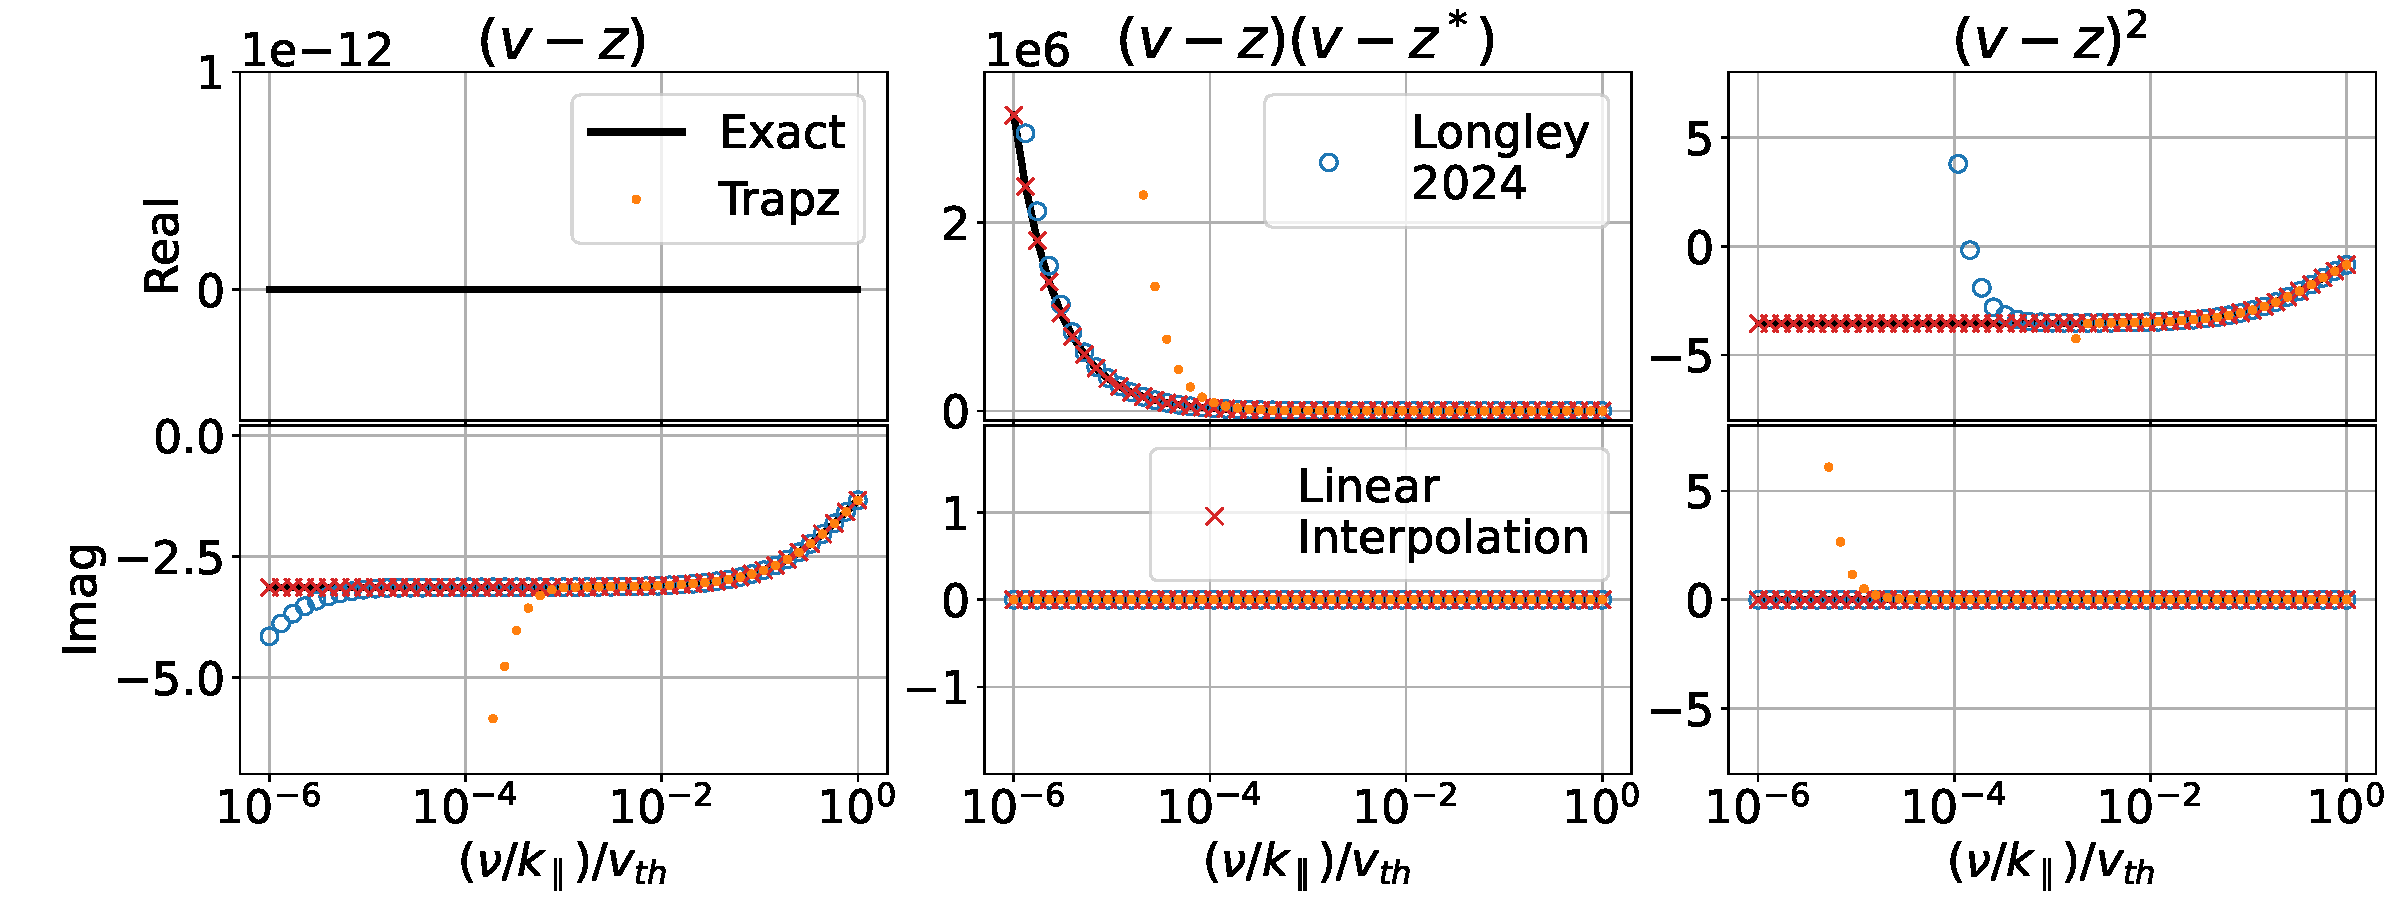
\includegraphics[width=\linewidth]{poleIntegrate_error_pole0_-3.pdf}
	\caption{Same as Fig.~\ref{f:poleIntegrateError0_pole0} but with $\Delta v_\parallel/v_{th}=10^{-3}$.}
	\label{f:poleIntegrateError-3_pole0}
\end{figure}

\begin{figure}[!htb]
	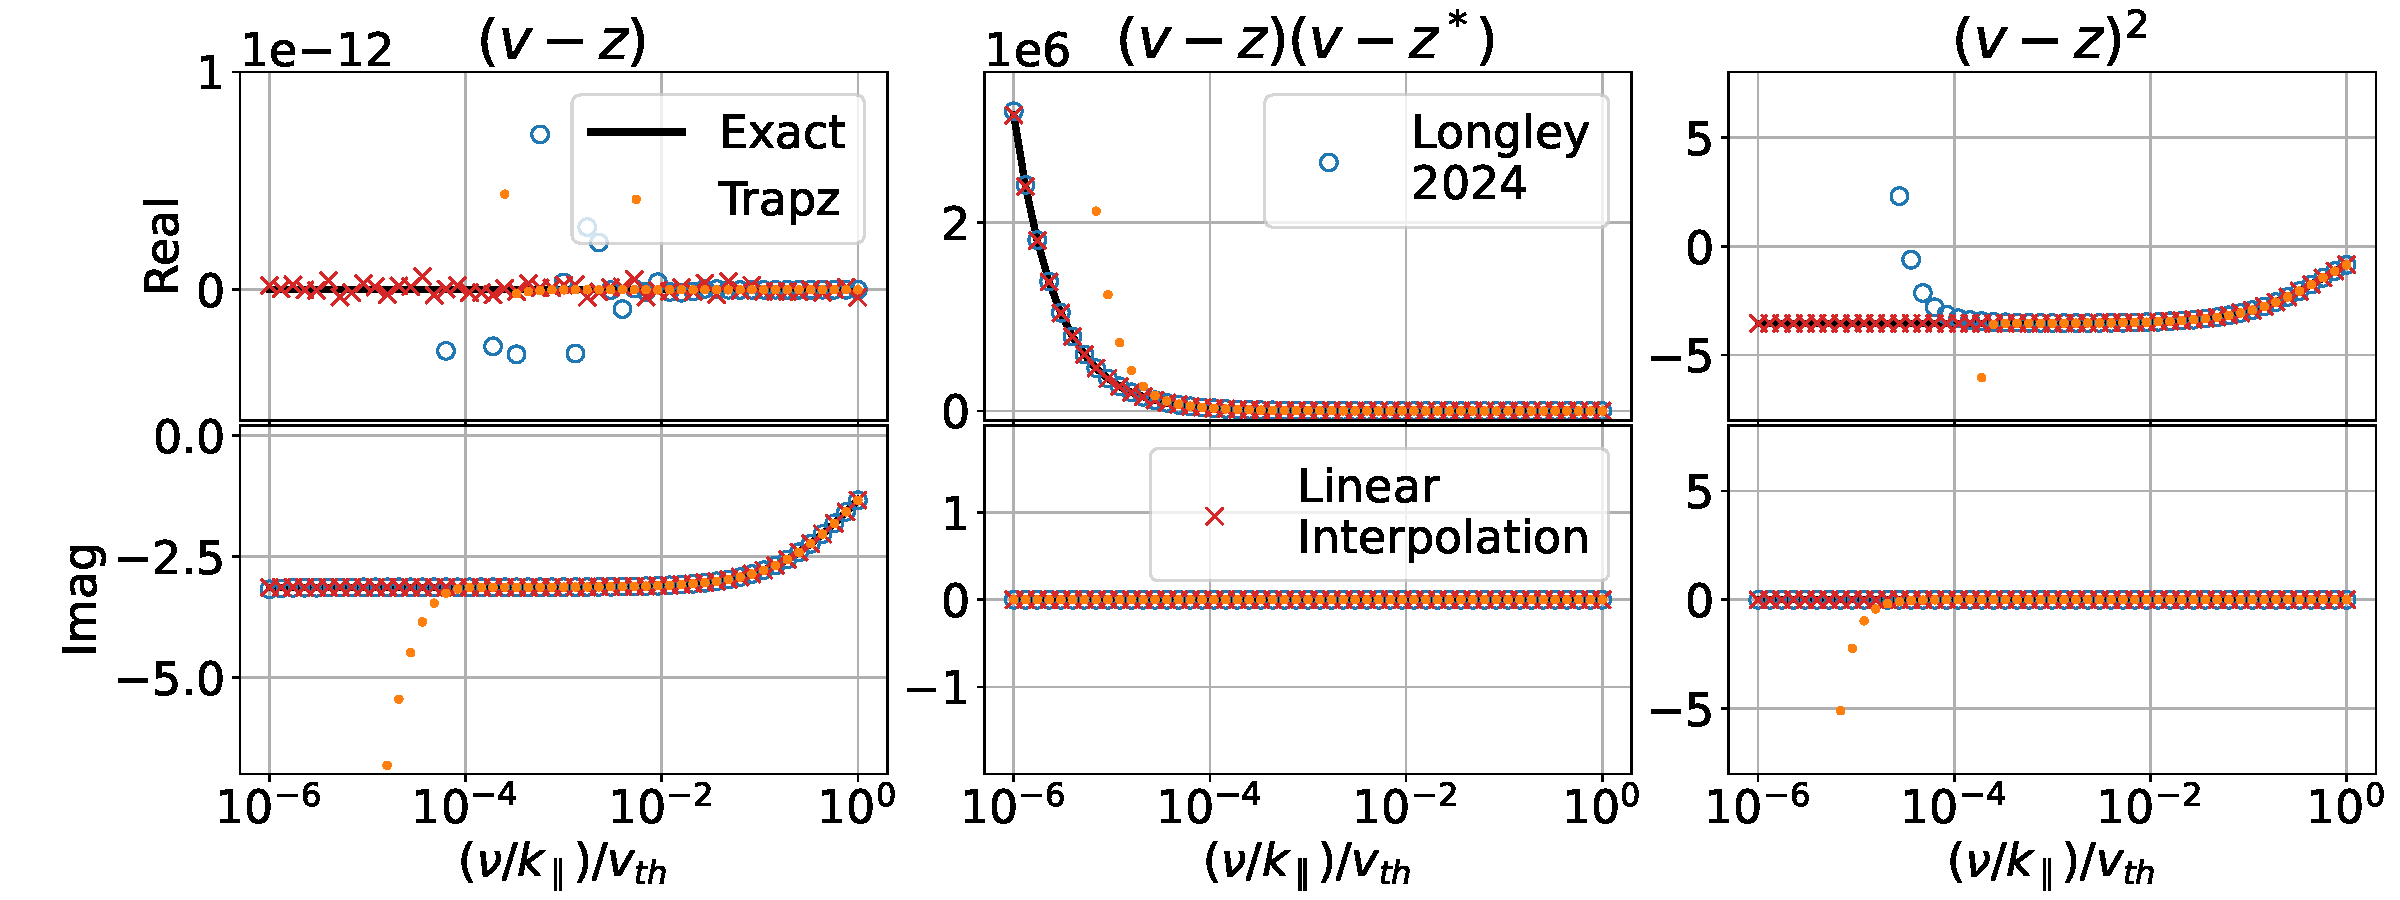
\includegraphics[width=\linewidth]{poleIntegrate_error_pole0_-4.pdf}
	\caption{Same as Fig.~\ref{f:poleIntegrateError0_pole0} but with $\Delta v_\parallel/v_{th}=10^{-4}$.}
	\label{f:poleIntegrateError-4_pole0}
\end{figure}

\begin{figure}[!htb]
	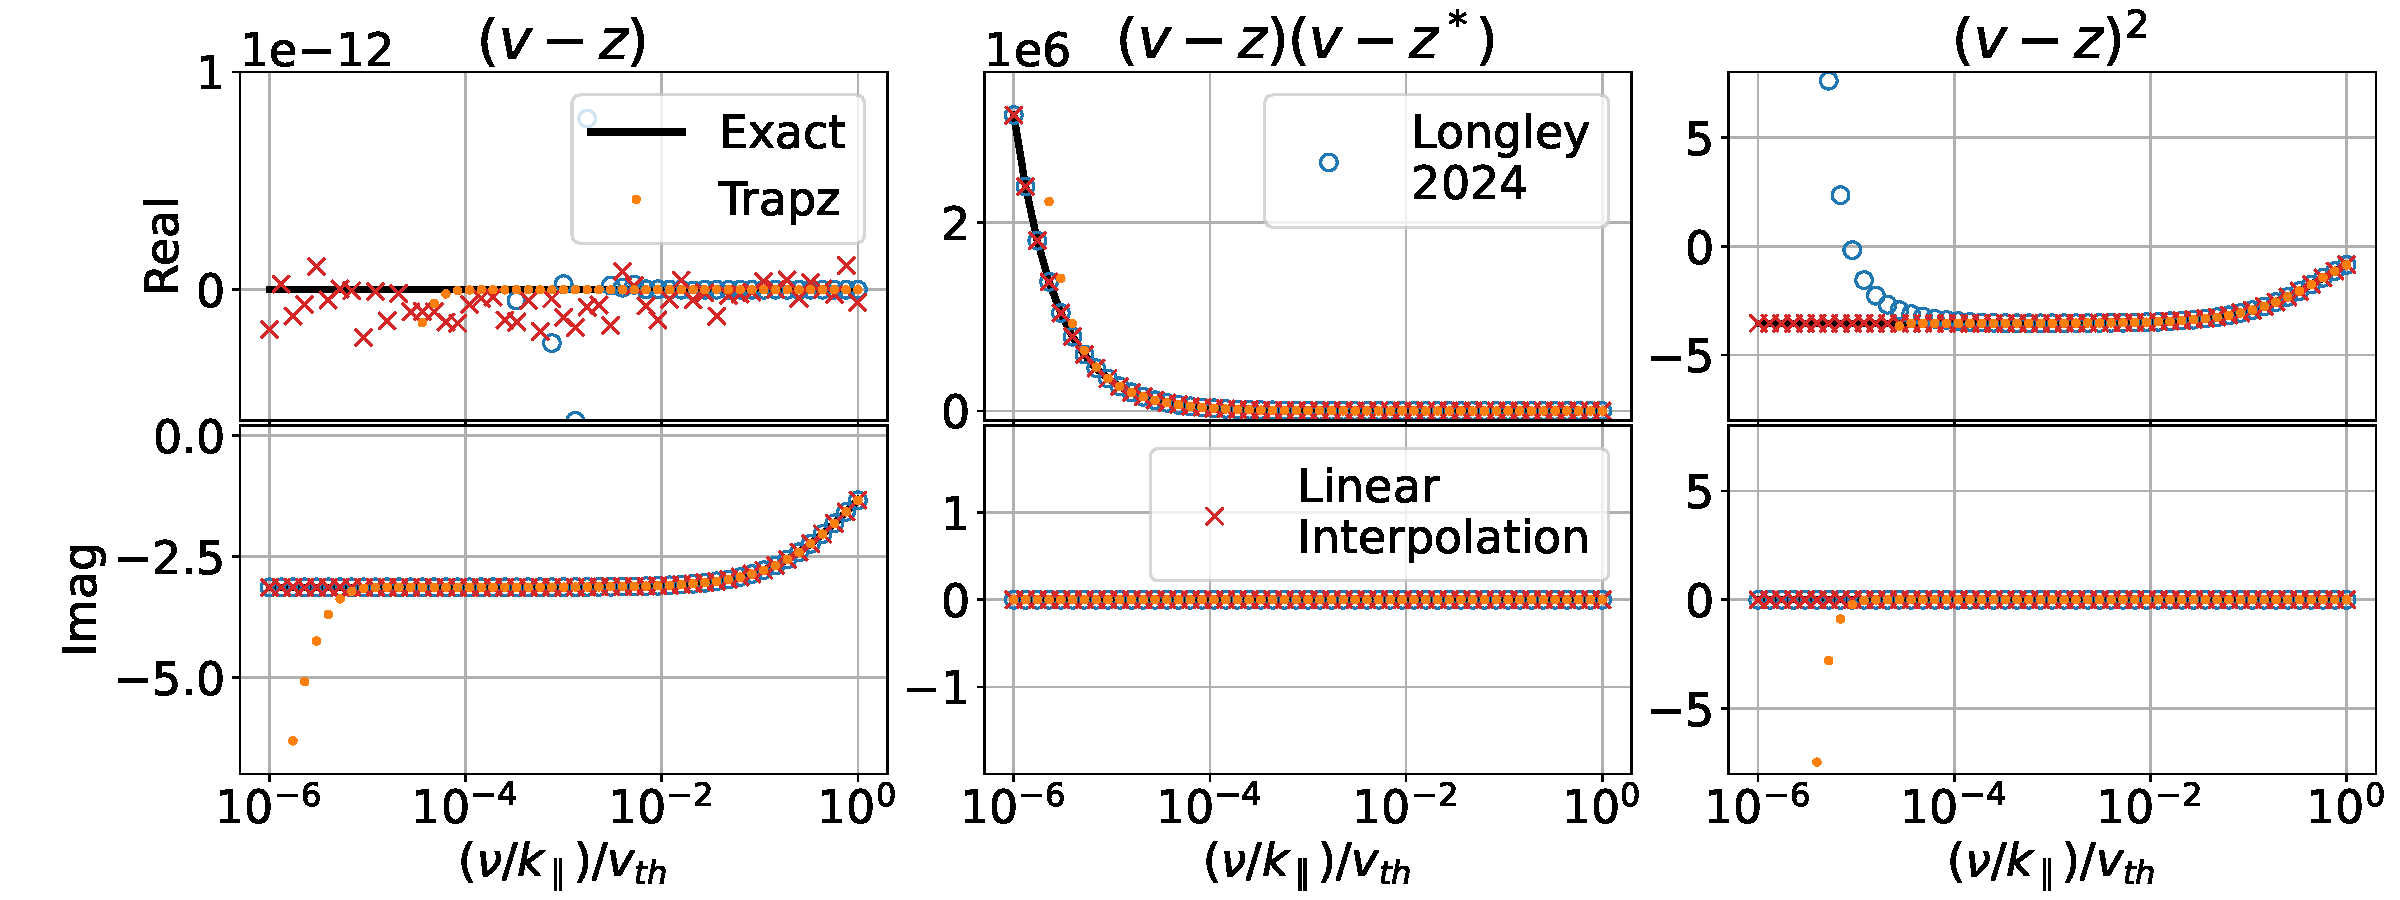
\includegraphics[width=\linewidth]{poleIntegrate_error_pole0_-5.pdf}
	\caption{Same as Fig.~\ref{f:poleIntegrateError0} but with $\Delta v_\parallel/v_{th}=10^{-5}$.}
	\label{f:poleIntegrateError-5_pole0}
\end{figure}


% Should we have a discussion somewhere about the merits of this method vs a quadrature approach? 
% I think one of the main pros to our method is that we don't need to worry beforehand about quadrature points and can have any arbitrary non-uniform mesh
% Further, to use quadrature, one needs to rewrite everything as Legendre polynomials yeah?
% If you are already doing it as a polynomial, then you can already use our method since it works for any arbitrary order polynomial. 
% I will show that somewhere too. The answer to these poles using the hypergeometric series solution from Mathematica. I first need to learn mroe and understand it though


\subsection{Extending to Arbitrary Polynomial Order}

Suppose instead of obtaining the distribution function as a discrete set of points (as one would in outputs of Monte Carlo, PIC, or finite discretization methodss), we have a solution with a polynomial representation (like those of spectral, Galerkin, and discontinuous Galerkin methods). 
For this work, we will only consider a discontinuous Galerkin approach, but the idea should is easily extended to global spectral represenations of the distribution function.
Consider a set of piecewise polynomial representations of the distribution as
\begin{equation}
	f_{0s,j}(v_\perp, v_\parallel) = c_0(v_\perp) + c_1(v_\perp) v_\parallel + c_2(v_\perp) v_\parallel^2 + \cdots + c_n(v_\perp) v_\parallel^n,
	= \sum_{m=0}^n c_m(v_\perp) v_\parallel^m
	\label{eq:arb_poly_dist} 
\end{equation}
where $c_j(v_\perp)$ are the polynomial coefficients for a polynomial of order $n$. 
Note that these coefficients are still functions of $v_\perp$ since we are only doing the pole integration in the parallel direction.
Thus, we can split the integral of the distribution function at some pole (we will use Eq.~\ref{eq:p1} as an example) into $n$ different integrals:
\begin{equation}
	\int \frac{f_{0s,j}(v_\perp, v_\parallel)}{v_\parallel -z} dv_\parallel = 
	\sum_{m=0}^n c_m(v_\perp)\int \frac{v_\parallel^m}{v_\parallel -z} dv_\parallel.
\end{equation}
 
In a similar way to Eqs.~\ref{eq:p1j}-\ref{eq:p2j}, we can obtain the indefinite integrals for each of these poles using the representation of the distribution function in Eq.~\ref{eq:arb_poly_dist} as
\begin{equation}
	p_1^j(v_\perp,v_\parallel) = \int \frac{f_{0s,j}(v_\perp, v_\parallel)}{v_\parallel-z} dv_\parallel = 
	\sum_{m=0}^n c_m(v_\perp) \frac{v_\parallel^{m+1}}{(m+1)z} \ _2F_1\bigg(1, m+1; m+2; \frac{v_\parallel}{z}\bigg)
	\label{eq:p1j_arb_poly}
\end{equation}
\begin{multline}
	p_*^j(v_\perp,v_\parallel) = \int \frac{f_{0s,j}(v_\perp, v_\parallel)}{(v_\parallel-z)(v_\parallel-z^*)} dv_\parallel \\
	= \sum_{m=0}^n c_m(v_\perp)
	\frac{v_\parallel^{m+1}}{2 i (m+1) |z|^2 \im(z)} 
	\Bigg[z \ _2F_1\bigg(1, m+1; m+2; \frac{v_\parallel}{z^*}  \bigg)  - z^* \ _2F_1\bigg(1, m+1; m+2; \frac{v_\parallel}{z}  \bigg)\Bigg]
	\label{eq:pstarj_arb_poly}
\end{multline}
\begin{equation}
	p_2^j(v_\perp,v_\parallel) = \int \frac{f_{0s,j}(v_\perp, v_\parallel)}{(v_\parallel-z)^2} dv_\parallel = 
	\sum_{m=0}^n c_m(v_\perp) \frac{v_\parallel^{m+1}}{(m+1)z^2} \ _2F_1\bigg(2, m+1; m+2; \frac{v_\parallel}{z}\bigg),
	\label{eq:p2j_arb_poly}
\end{equation}
where $_2F_1(a, b; c; z)$ is the hypergeometric function. % rethink how I want to say this.
% Add how to do this in python briefly

Track down how other people have done the plasma dispersion relation calculation and see what their applications have been for.



\subsection{Calculating temperature in arbitrary direction}
\label{s:equiv-temp-known}

This section discusses numerical methods used to calculate the temperature in an arbitrary direction.
From a practical perspective, we can use this to get the line of sight temperature, which is what a radar will see.
For an arbitrary distribution function, we can back out the temperature from its zeroth, first, and second moments in the line of sight velocity direction, $k$:
\begin{align}
	M_0 &= \int f d\mathbf{v} \label{eq:M0}\\
	M_{1_k} &= \int v_k f d\mathbf{v} \label{eq:M1} \\
	M_{2_{kk}} &= \int v_k^2 f d\mathbf{v}. \label{eq:M2}
\end{align}
From Eq.~\ref{eq:M0}-\ref{eq:M2}, we can calculate the temperature (assuming $v_{th}=\sqrt{2k_BT_k/m}$) in the line of sight direction as
\begin{equation}
	T_k = \frac{m}{k_B} \Bigg[ \frac{M_{2_{kk}}}{M_0}  - \bigg( \frac{M_{1_k}}{M_0} \bigg)^2\Bigg].
	\label{eq:Tk_full}
\end{equation}
For a Maxwellian distribution, you will find that this exactly backs out the temperature.
For a non-Maxwellian distribution, this will find the line of sight temperature equivalent (temperature can become ill defined for non-Maxwellian distributions).
In our case, we are using normalized distribution functions such that their zeroth moment (Eq.~\ref{eq:M0}) is 1 yielding
\begin{equation}
	T_k = \frac{m}{k_B} (M_{2_{kk}} - M_{1_k}^2).
	\label{eq:Tk_simp}
\end{equation}
All of our distributions we will be looking at are azimuthally symmetric. 
Furthermore, most (if not all) of the distributions we will consider are symmetric about the perpendicular plane where $v_\parallel=0$.
In this case, the first moment (Eq.~\ref{eq:M1}) is 0 giving an even further simplified 
\begin{equation}
	T_k = \frac{m M_{2_{kk}}}{k_B}.
	\label{eq:Tk_full_simp}
\end{equation}
Thus, all we need to do is figure out how to calculate the second moment in the line of sight direction.

\subsubsection{Known Distribution Function}
If we already know the functional form of the distribution function, then we can do some coordinate transformations to properly calculate Eq.~\ref{eq:Tk_full_simp}. 
Assume we have a Cartesian grid with coordinates $v_x$, $v_y$, and $v_z$.  % Have a pic of this in here eventually
Since we are only looking at azimuthally symmetric distribution function, it is convenient to use cylindrical coordinates in the form of $v_\parallel$ and $v_\perp$ with the directions being respective to the magnetic field.
For simplicity, let us assume that the parallel direction is in the direction of $v_z$.
Let us now consider a different coordinate system we call $v_x'$, $v_y'$, and $v_z'$ with $v_z'$ being in the line of sight direction.


Our goal is to write the orignal $v_{x,y,z}$ system in terms of the $v_{x,y,z}'$ system. 
By azimuthal symmetry and since we only care about how the temperature varies with angle respective to the magnetic field, the prime coordinate system, $v_{x,y,z}'$, is just a rotation of the original coordinate system, $v_{x,y,z}$, by $-\theta$ about the $v_x$ axis. 
Thus, to go the other way, the original coordinate system, $v_{x,y,z}$ can be found by rotating the prime coordinate system, $v_{x,y,z}'$, by $\theta$ about the $v_x'$ axis.
The standard rotation matrix for such a transformation is
\begin{equation}
	\mathbf{R}_{v_x}(\theta) = \begin{bmatrix}
		1 & 0 & 0 \\
		0 & \cos\theta & -\sin\theta \\
		0 & \sin\theta & \cos\theta
	\end{bmatrix}.
	\label{eq:rot_mat}
\end{equation}
Therefore, we can write the original coordinate system, $v_{x,y,z}$ in terms of the prime system, $v_{x,y,z}'$ as
\begin{equation}
	\begin{bmatrix}
		v_x \\ v_y \\ v_z
	\end{bmatrix} = 
	\mathbf{R}_{v_x} \begin{bmatrix}
		v_x' \\ v_y' \\ v_z'
	\end{bmatrix} = 
	\begin{bmatrix}
		v_x' \\
		v_y'\cos\theta - v_z'\sin\theta \\
		v_y'\sin\theta + v_z'\cos\theta
	\end{bmatrix}.
\end{equation}
Now, we must convert to cylindrical coordinates. 
We set $v_z$ to be in the parallel direction; therefore,
\begin{equation}
	v_\parallel = v_z = v_y'\sin\theta + v_z'\cos\theta.
\end{equation}
The perpendicular direction is just the radius giving
\begin{equation}
	v_\perp = \sqrt{v_x^2+v_y^2}
	= \sqrt{v_x'^2 + (v_y'\cos\theta - v_z'\sin\theta)^2 }.
\end{equation}
Based on these, we can effectively write any function of $v_\perp$ and $v_\parallel$ in terms of $v_{x,y,z}'$.
Thus, the second moment in the line of sight direction ($v_z'$) becomes
\begin{equation}
	M_{2_{z'z'}} = \int v_z'^2 f d\mathbf{v}'.
\end{equation}


\subsubsection{Unknown Distribution Function}


	\chapter{Results}

\section{Maxwellian}

These are parameters for the calculation in Fig.~\ref{f:compareMaxwellian}.
Angle is $60^\circ$. 
Radar frequency is \SI{230}{\mega\hertz} which corresponds to EISCAT VHF and EISCAT 3D radars.  % Citation here?
Magnetic field strength is $10^{-5}$ \si{\tesla}.
The neutral, ion, and electron temperature are all $T_i=T_e=T_n=\SI{1000}{\kelvin}$.
The neutral number density is \SI{1.8e14}{\meter^{-3}}.
The plasma is quasineutral with $n_i=n_e=10^9$ \si{\meter^{-3}}.
Atomic oxygen is the ion species.
The numerical calculation is done using $n_{\max}$ of 2000 for the ions and 50 for the electrons (these two are expected to be overkill for the calculation).

\begin{figure}[!htb]
	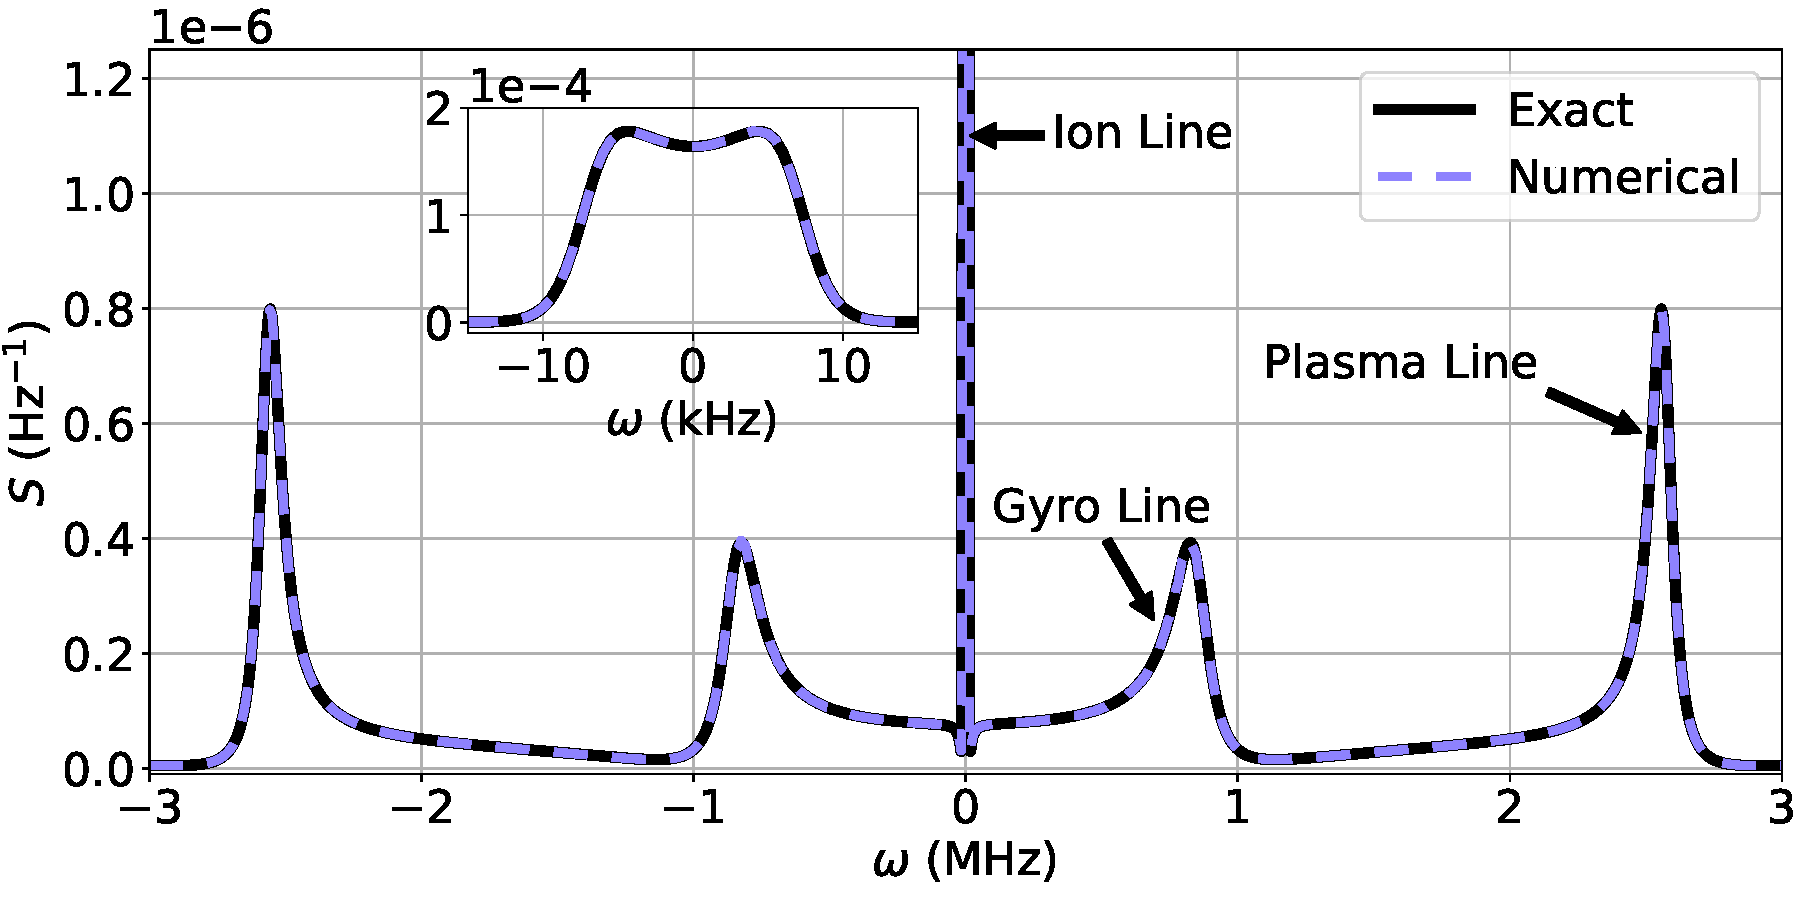
\includegraphics[width=\linewidth]{compareMaxwellian.pdf}
	\caption{Comparison between exact solution and numerical solution for a Maxwellian plasma.}
	\label{f:compareMaxwellian}
\end{figure}


\section{Toroidal}

\begin{equation}
	f_0 = \frac{
		\exp\bigg( - \frac{2 D^* v_\perp}{v_{th,\perp}} \bigg) I_0 \bigg(  \frac{2 D^* v_\perp}{v_{th,\perp}} \bigg)  
		\exp \bigg(  -\frac{v_\parallel^2}{v_{th,\parallel}^2} - \Big[ \frac{v_\perp}{v_{th,\perp} } - D^* \Big]^2  \bigg)}{
		\pi^{3/2} v_{th,\parallel} v_{th,\perp}^{2}}
	\label{eq:toroidal_dist}
\end{equation}

These plots were made using Eq.~\ref{eq:toroidal_dist} as the base distribution with the exact parameters from \cite{goodwin2018} for the background plasma and radar parameters.
The equivalent temperature Maxwellian is calculated using the method in Sec.~\ref{s:equiv-temp-known}.

\begin{figure}[!htb]
	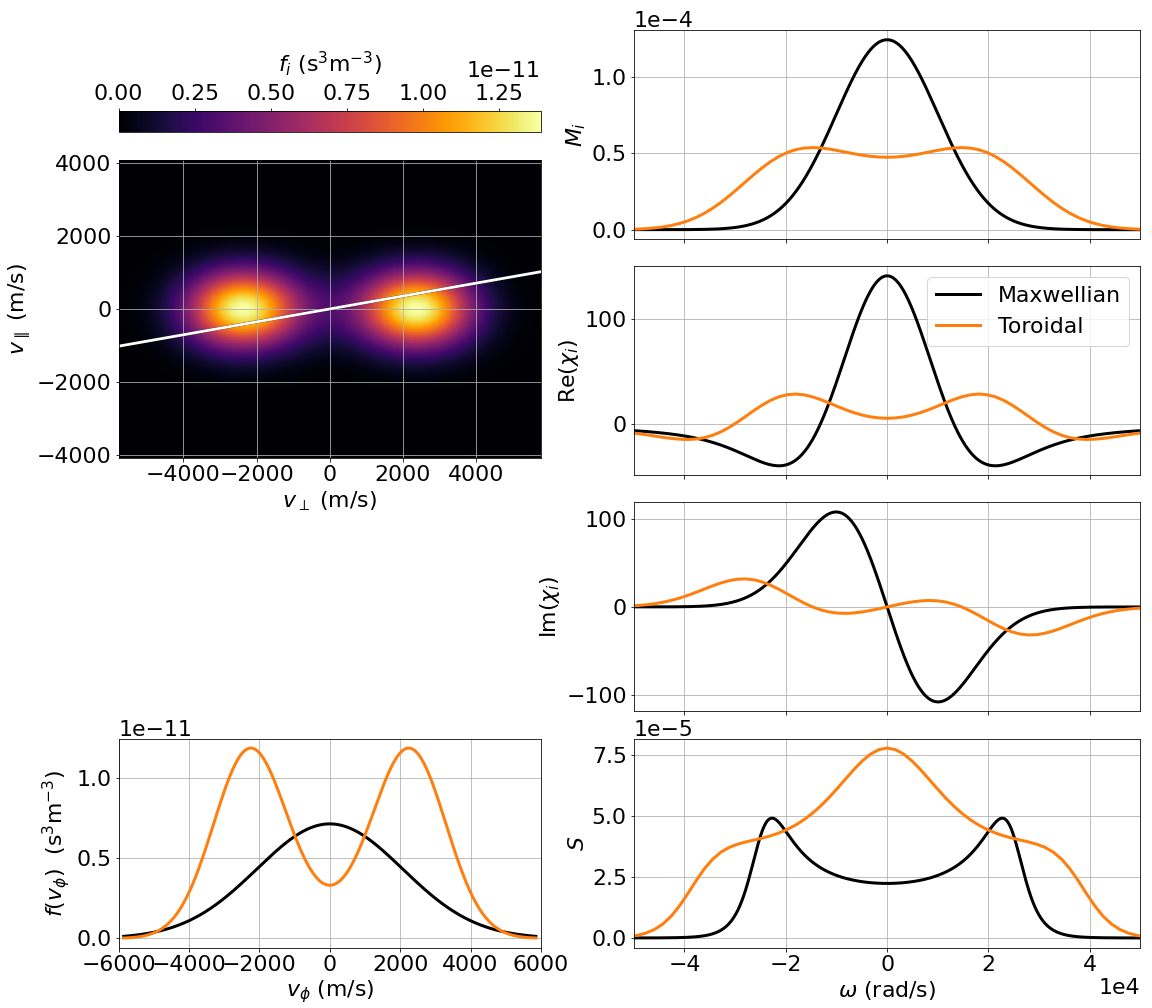
\includegraphics[width=\linewidth]{par2.3_perp2_Goodwin_Te4000_theta80_spectrum.png}
	\caption{Plots of plasma with toroidal ion distribution (orange line) compared to the equivalent temperature Maxwellian (black line).
	Color plot is the 2D $v_\perp v_\parallel$ representation of the distribution function from Eq.~\ref{eq:toroidal_dist}.
	The line on the color plot is the radar wave vector direction.
	The bottom left panel is the distribution function along wavevector direction.
	The top right panel is the modified distribution function.
	The middle right panels are the real and imaginary parts of the ion susceptibility, respectively.
	The bottom right panel is the ISR spectrum.
	The triple hump is shown, as expected based on \cite{goodwin2018}.}
	\label{f:toroidal}
\end{figure}


\section{Kappa}

These are results for a kappa distribution. See the \verb*|kappa_dist.nb| These have the form from \citep{livadiotis2015} as
\begin{equation}
	f_\kappa(\mathbf{v}) \sim \Bigg[   
	1 + \frac{1}{\kappa-d/2} \frac{\mathbf{v}^2}{v_{th}^2}
	\Bigg]^{-\kappa-1},
	\label{eq:kappa_base}
\end{equation}
where $\kappa$ is a constant that determines how long the tail of the distribution is (lower number means more high energy particles),
$v_{th}=\sqrt{2k_BT/m}$ is the thermal velocity,
and $d$ is the number of degrees of freedom (for our case, $d=3$).

In cylindrical coordinates, the square of the velocity becomes $\mathbf{v}^2=v_\perp^2+v_\parallel^2$. 
The normalization factor is found by taking the reciprocal of zeroth moment of Eq.~\ref{eq:kappa_base}.
Thus, the total disitribution function with three degrees of freedom is
\begin{equation}
	f_{\kappa}(v_\perp,v_\parallel) = 
	\frac{1}{\pi^{\frac{3}{2}} v_{th}^3 \big(\kappa-\frac{3}{2}\big)^{\frac{5}{2}}}
	\frac{\Gamma\big(\kappa+1\big)}{\Gamma\big(\kappa-\frac{3}{2}\big)}
	\Bigg( 1 + \frac{1}{\kappa-\frac{3}{2}} \frac{v_\perp^2+v_\parallel^2}{v_{th}^2}
	\Bigg)^{-\kappa-1},
	\label{eq:kappa_dist}
\end{equation}
where $\Gamma$ is the Gamma function.
Thus, based on the denominator Gamma term in this formulation, we can see that $kappa>3/2$ because the Gamma function is defined only for $z>0$.
As $\kappa\rightarrow\infty$, Eq.~\ref{eq:kappa_dist} tends to the Maxwellian distribution.
Furthermore, the temperature of this formulation of the kappa distribution is the same as that of the Maxwellian. 
In other words, the second moment is related to the thermal velocity in the same manner as in Maxwellian:
\begin{equation}
	\int_{-\infty}^\infty f_{\kappa}(v_\perp,v_\parallel) (v_\perp^2+v_\parallel^2) v_\perp dv_\perp dv_\parallel d\phi = 
	\frac{3}{2} v_{th}.
\end{equation}

% Throw some example plots of the kappa distribution here









	
	
	
	
	%\bibliographystyle{plainnat}
	\bibliography{reference}
	\addcontentsline{toc}{section}{Reference}
	
	\begin{appendices}
		\chapter{Pole Integration Testing}

Put all of my tests here. 

\section{Testing functions used within poleIntegrate}

% Redo these tests, these are all now wrong that we changed the bounds of the outer part of the mesh refinement
\subsection{test\_getVInterp}
For \verb|test_getVInterp|, we have two poles at $2+i$ and $3-2i$ 
and an input velocity mesh of ranging from 0 to 10 in increments of 0.1.
Based on this, we can manually calculate that the expected velocity mesh for a \verb|mesh_n| of 11 to be
[0, 0.4, 0.6, 0.8, 1, 1.2, 1.4, 1.6, 2, 2.2, 2.4, 2.8, 3, 3.2, 3.6, 3.8, 4, 4.6, 4.8, 5, 5.4, 5.6, 6, 6.2, 6.4, 7, 7.2, 8, 8.6, 8.8, 9, 9.6, 10]. 
This has been tested and the function works as intended.

\subsection{test\_getIntegrand}
For \verb|test_getIntegrand|, we are trying to calculate 
\begin{equation}
	\frac{f_0(v)}{\prod_j (v-p_j)^{\mathcal{O}_j}},
	\label{eq:a_integrand}
\end{equation}
where $f_0(v)$ is the distribution function and $p_j$ are the poles with orders $\mathcal{O}_j$.
For an input of velocity of [0,1,2], an input distribution function of [2,3,1]
and two poles at $2+i$ and $3-2i$ with orders 1 and 2 respectively. 
Plugging these values into Eq.~\ref{eq:a_integrand} and using WolframAlpha, we get that the integrand should be
[$-0.05207-0.04497i$ ,$-0.1875-0.1875i$, $-0.16-0.12i$].
This has been tested and the function works as intended.

\subsection{test\_plemelj}

The exact solution for the integral over the real axis is provided by the Plemelj theorem, % Make a note on section whatever for where we talk about this more.
and is 
\begin{equation}
	\int_{-\infty}^\infty \frac{f_0(v)}{\prod_j (v-p_j)^{\mathcal{O}_j}} = 
	i \pi \sum_j \frac{ \sgn(\im[p_j]) f(\re[p_j])}{ \prod_{j\neq k} (p_j - p_k)^{\mathcal{O}_j}}.
	\label{eq:a_plemelj}
\end{equation} 
This solution is technically for the limit as the poles approach the real axis. 
Nevertheless, we can use it to test the numerical integration.
For a velocity mesh of [1, 2, 3], 
poles of $2-i$, $3+2i$, and $1-5i$ with orders 
1, 2, and 1, respectively, the exact solution using Eq.~\ref{eq:a_plemelj} (and WolframAlpha) is
\begin{equation}
	\int_{-\infty}^\infty \frac{f_0(v)}{\prod_j (v-p_j)^{\mathcal{O}_j}} = 
	i \pi \bigg(-\frac{11+7i}{170} \verb|Fv[1]| + \frac{96+247i}{140450} \verb|Fv[2]|  + \frac{26+15i}{901} \verb|Fv[0]|  \bigg) 
\end{equation}
This has been tested and the function works as intended.


\section{Testing poleIntegrate}

To test the pole integration, we will use a Guassian for the distribution function,
\begin{equation}
	f_0(v) = \exp(-v^2). 
	\label{eq:norm_var_maxwellian}
\end{equation}
One can think of this as examining a Maxwellian distribution with a velocity variable normalized by the thermal velocity.
For obtaining the incoherent scatter spectra, we will need to use this pole integration for integrands 
with singular poles at some $a+\gamma i$ as well as integrands with double poles at $a\pm \gamma i$.
%In addition, the Plemelj theorem holds true in the limit as $\gamma$ approaches zero. 
Therefore, we will make plots of the integrals as functions of $\gamma$ to show this.
For our case, we will have $\gamma$ vary and let $a=0.25$. 
To relate this back to Eqs. (REF HERE), the imaginary component of the poles is $-\nu/k_\parallel$.
For a proper comparison with the normalized variable Maxwellian in Eq.~\ref{eq:norm_var_maxwellian},
we will let $\gamma = -(\nu/k_\parallel)/v_{th}$. 
Therefore, the following plots can provide guidance on the velocity resolution needed to obtain accurate results.		
Please see the Mathematica notebook \verb*|exact_poleIntegrate.nb| for the analytic solutions to these integrals. % Reword

For a singular pole at $z$, the exact solution is
\begin{equation}
	p_1(z) = \int_{-\infty}^\infty \frac{f}{v-z} dv = 
	\exp(-z^2) \Bigg[ -\pi \erfi(z) + \ln \Big(-\frac{1}{z}\Big) + \ln\Big(\frac{1}{z}\Big)\Bigg]\\
	\label{eq:exact_single_pole}
\end{equation}
For utility later with the other solutions, we will call this solution $p_1(z)$.

\begin{figure}[!htb]
	\centering
	\includegraphics[width=\linewidth]{p1.pdf}
	\caption{Comparisons for a single pole integral calculation *Eq.~\ref{eq:exact_single_pole})
		between the pole refined mesh integration function we made (blue circles), % Eventually say that better 
		a naive trapezoidal integration not considering effects of poles (orange dots), and
		the exact solution described by Eq.~\ref{eq:exact_single_pole} (black line)
		for varying $\Delta v$.}
	\label{f:single_pole_comparison}
\end{figure}

Fig.~\ref{f:single_pole_comparison} shows how our pole integration compares with 
a naive trapezoidal integration and the exact solution from Eq.~\ref{eq:exact_single_pole},
as the pole approaches the real axis.
The approximate calculation uses a refined mesh of 101 points. 
It was found that additional points did not affect the solution in an appreciable way regardless of choice of $\Delta v$.
For large $\Delta v$, our pole integration clearly provides a better result
compared to the naive trapezoidal integration. 
As the $\Delta v$ decreases, both our approximation and the naive calculation improve.
For sufficiently small $\Delta v$, within the range of $\gamma$ chosen, both our
approximation and the naive solution converge.


For a double pole at $v - z$ and $v-z^*$ (where $z^*$ is the complex conjugate of $z$), the analytical solution to the integral is
\begin{equation}
	\int_{-\infty}^\infty \frac{\exp (-v^2)}{(v-z)(v-z^*)} dv = 
	\frac{i \Big[ g(z^*) - g(z)  \Big]}{2 \im(z)},
	\label{eq:exact_double_pole}
\end{equation}
where $g(z)$ is the solution to the single pole integrand (Eq.~\ref{eq:exact_single_pole}).


Fig.~\ref{f:double_pole_comparison} shows the comparisons to the exact solution for varying $\Delta v$.
Here, we find that the finer mesh pole integration, for all $\Delta v$, correctly calculates that the 
imaginary component of the solution is zero.
The naive trapezoidal integration gets better with lower $\Delta v$, but still does not reach anything close to zero.
For the real part of the solution, however, the finer mesh approximation we use does worse 
than the naive integration. While hte naive integration is still incorrect, it is less incorrect than the pole refined mesh integration.
Thus suggests for these double poles, we want to be the pole to be further from the real axis to obtain an accurate solution
with the pole refined mesh integration. 
Otherwise, perhaps the solution is to use the pole refined mesh integration for the imaginary component and the naive trapezoidal integration for the real component.

\begin{figure}[!htb]
	\centering
	\begin{subfigure}{.32\textwidth}
		\includegraphics[width=\linewidth]{Gaussian_vs_Plemelj_changeGamma_doublePole_1e0}
		\caption{$\Delta v = 10^0$}
	\end{subfigure}
	\begin{subfigure}{.32\textwidth}
		\includegraphics[width=\linewidth]{Gaussian_vs_Plemelj_changeGamma_doublePole_1e-1}
		\caption{$\Delta v = 10^{-1}$}
	\end{subfigure}
	\begin{subfigure}{.32\textwidth}
		\includegraphics[width=\linewidth]{Gaussian_vs_Plemelj_changeGamma_doublePole_1e-2}
		\caption{$\Delta v = 10^{-2}$}
	\end{subfigure}
	\begin{subfigure}{.32\textwidth}
		\includegraphics[width=\linewidth]{Gaussian_vs_Plemelj_changeGamma_doublePole_1e-3}
		\caption{$\Delta v = 10^{-3}$}
	\end{subfigure}
	\begin{subfigure}{.32\textwidth}
		\includegraphics[width=\linewidth]{Gaussian_vs_Plemelj_changeGamma_doublePole_1e-4}
		\caption{$\Delta v = 10^{-4}$}
	\end{subfigure}
	\begin{subfigure}{.32\textwidth}
		\includegraphics[width=\linewidth]{Gaussian_vs_Plemelj_changeGamma_doublePole_1e-5}
		\caption{$\Delta v = 10^{-5}$}
	\end{subfigure}
	\caption{Comparisons for a double pole integral calculation
		between the pole refined mesh integration function we made (blue solid line), % Eventually say that better 
		a naive trapezoidal integration not considering effects of poles (orange dots), 
		the exact solution described by Eq.~\ref{eq:exact_double_pole} (red dashed lined), 
		and the Plemelj limit described by Eq.~\ref{eq:a_plemelj} (black dashed line)
		for varying $\Delta v$.}
	\label{f:double_pole_comparison}
\end{figure}

For a single pole at $z$ with order 2, the analytical solution to the integral is. 
% Do this test at some point
\begin{equation}
	\int_{-\infty}^\infty \frac{ \exp(-v^2) }{(v-z)^2} dv = - 2 \sqrt{\pi} - 2 z g(z).
\end{equation}


\section{Testing spectra calculations}
The following are tests to ensure the $U$, $M$, and $\chi$ are being calculated properly.
Then, if those are correct, we can properly calculate the resulting ISR spectra for a particular ion distribution function.







		\chapter{Derivations}

\section{$\ln(-1/z)-\ln(1/z)=\sgn\big[\im(z)\big]i\pi$}
\label{s:ln1z}

This section proves that for some complex number $z = a + bi$ with $b \neq 0$, then
\begin{equation}
	\ln\Big(-\frac{1}{z}\Big) - \ln\Big(\frac{1}{z}\Big) = \sgn[\im(z)\big] i \pi.
	\label{eq:ln1z}
\end{equation}
In general, we can use log laws to show that this is somewhat the case.
\begin{align}
	\ln\Big(-\frac{1}{z}\Big) - \ln\Big(\frac{1}{z}\Big) 
	&= \ln(-1) - \ln(z) - \big[ \ln(1) - \ln(z) \big] \nonumber \\
	&= i \pi - \ln(z) - 0 + \ln(z) \nonumber \\
	&= i \pi
\end{align}
This is slightly different than Eq~.\ref{eq:ln1z} by a 
factor of $\sgn(b)$. 
Generally, this should be fine because complex logarithms are multi-valued functions
that are defined by the primary choice of angle plus $2 n \pi$ where $n$ is an arbitrary integer.
However, when doing the actual calculation (with actual numbers in Python or Mathematica), 
we find that the primary choice of angle is dependent on the sign of $b$.
Thus, we will prove this dependency here and thus simplify our solutions significantly.

Consider a complex number $z=a+bi$ with $b \neq 0$. 
We can rewrite this in exponential form as $z = r_0 \exp(i \theta_0)$.
We can obtain the angle $\theta_0$ by obtaining the argument of the complex number, 
or in others taking the inverse tangent.
However, we want the range of the inverse tangent to be in $(-\pi,\pi]$ instead
of the usual $(-\pi/2,\pi/2)$.
Therefore, we will use the $\atan2$ function, or the two argument inverse tangent function
that includes information about the quadrant of the complex number.
Thus, the angle is defined fully as the following depending on several characteristics of $a$ and $b$.
Table~\ref{t:theta0} shows how to obtain $\theta_0$ based on where $z$ is on the complex plane.
We can also get what $\tan^{-1}(b/a)$ is in terms of $\theta_0$, which will be important for 
proving Eq.~\ref{eq:ln1z}.
\begin{table}[H]
	\centering
	\caption{Obtaining $\theta_0$ based on $\atan2$ function depending on location of $z$ in the complex plane.
		Then, we obtain $\tan^{-1}(b/a)$ in terms of $\theta_0$, which is used for future calculations.
		Note we assume that $b\neq0$.}
		\label{t:theta0}
	\begin{tabular}{c|c|c|c}
	\makecell[t]{\textbf{Quadrant \RN{2}}\\
		$a<0\ \&\ b > 0$ \\
		$\theta_0 = \tan^{-1} \big( \frac{b}{a} \big) + \pi$ \\
		$\tan^{-1} \big( \frac{b}{a} \big) = \pi - \theta_0$  \vspace{2pt}}
	&
	\makecell[t]{\textbf{Positive Complex Axis} \\
		$a=0\ \&\ b > 0$ \\
		$\theta_0 = \frac{\pi}{2}$ }
	&
	\makecell[t]{\textbf{Quadrant \RN{1}}\\
		$a>0\ \&\ b > 0$ \\
		$\theta_0 = \tan^{-1} \big( \frac{b}{a} \big)$ \\}
	&
	\makecell[t]{\textbf{Positive Real Axis}\\
	$a> 0\ \&\ b = 0$ \\
	$\theta_0 = 0$
	}
	\\
	\hline
	\makecell[t]{\textbf{Quadrant \RN{3}}\\
		$a<0\ \&\ b < 0$ \\
		$\theta_0 = \tan^{-1} \big( \frac{b}{a} \big) - \pi$ \\
		$\tan^{-1} \big( \frac{b}{a} \big) = -\pi - \theta_0$  }
	&
	\makecell[t]{\textbf{Negative Complex Axis} \\
		$a=0\ \&\ b < 0$ \\
		$\theta_0 = -\frac{\pi}{2}$ }
	& 
	\makecell[t]{\textbf{Quadrant \RN{4}}\\
		$a> 0 \ \&\ b < 0$ \\
		$\theta_0 = \tan^{-1} \big( \frac{b}{a} \big)$ \\} 
	&
	\makecell[t]{\textbf{Negative Real Axis}\\
		$a < 0\ \&\ b = 0$ \\
		$\theta_0 = \pi$
	}
	\end{tabular}
\end{table}
It is not $z$ that shows up in Eq.~\ref{eq:ln1z} but $1/z$ and $-1/z$. 
So let us determine what these are. 
The reciprocal of $z$ is
\begin{equation}
	\frac{1}{z} =  \frac{1}{a+bi}.
\end{equation}
To get to an easy to use form, multiply the top and bottom by the complex conjugate of $z$
and then define $1/z$ as
\begin{equation}
	\frac{1}{z} = \frac{a-bi}{a^2 + b^2} = r_1 \exp(i \theta_1).
\end{equation}
Note how the angle of the reciprocal of $z$ is the same as the angle of the complex conjugate of $z$.
This is effectively saying that the quadrant that $1/z$ is in is flipped up/down.
Then, we can calculate $\theta_1$ in a similar way to how we did for $\theta_0$.
In addition, we can relate $\theta_1$ to $\theta_0$ through $\tan^{-1}(b/a)$ because the inverse tangent is an odd function.
Table~\ref{t:theta1} is a similar table to Table~\ref{t:theta0} and is based on where $z$ (note, not $1/z$) is in the complex plane.
\begin{table}[H]
	\centering
	\caption{Obtaining $\theta_1$ for $1/z$ based on $\atan2$ function depending on location of $z$ in the complex plane.
		Then we relate it back to $\theta_0$ through $\tan^{-1}(b/a)$ using the relationships from Table~\ref{t:theta0}.}
	\label{t:theta1}
	\begin{tabular}{c|c|c|c}
		\makecell[t]{\textbf{Quadrant \RN{2}}\\
			$a<0\ \&\ b > 0$ \\
			$1/z$ in Quadrant \RN{3} \\
			$\begin{aligned}
				\theta_1 
				&= \tan^{-1}\big(\tfrac{-b}{a} \big) - \pi \\
				&= - \tan^{-1}\big(\tfrac{b}{a} \big) - \pi \\
				&= -(\pi - \theta_0) - \pi \\
				&= \theta_0 - 2 \pi
			\end{aligned} $ }
		&
		\makecell[t]{\textbf{Positive Complex Axis} \\
			$a=0\ \&\ b > 0$ \\
			$1/z$ along negative complex axis \\
			$\theta_1 = -\frac{\pi}{2}$ }
		&
		\makecell[t]{\textbf{Quadrant \RN{1}}\\
			$a>0\ \&\ b > 0$ \\
			$1/z$ in Quadrant \RN{4} \\
			$\begin{aligned}
				\theta_1 
				&= \tan^{-1}\big(\tfrac{-b}{a} \big) \\
				&= -\tan^{-1}\big(\tfrac{b}{a} \big) \\
				&= -\theta_0
			\end{aligned}$}
		&
		\makecell[t]{\textbf{Positive Real Axis}\\
			$a> 0\ \&\ b = 0$ \\
			$1/z$ along positive real axis\\
			$\theta_1 = 0$
		}
		\\
		\hline
		\makecell[t]{\textbf{Quadrant \RN{3}}\\
			$a<0\ \&\ b < 0$ \\
			$1/z$ in Quadrant \RN{2} \\
			$\begin{aligned}
				\theta_1 
				&= \tan^{-1}\big(\tfrac{-b}{a} \big) + \pi \\
				&= - \tan^{-1}\big(\tfrac{b}{a} \big) + \pi \\
				&= -(-\pi - \theta_0) + \pi \\
				&= \theta_0 + 2 \pi
			\end{aligned} $}
		&
		\makecell[t]{\textbf{Negative Complex Axis} \\
			$a=0\ \&\ b < 0$ \\
			$1/z$ along positive complex axis \\
			$\theta_1 = \frac{\pi}{2}$ }
		& 
		\makecell[t]{\textbf{Quadrant \RN{4}}\\
			$a>0\ \&\ b > 0$ \\
			$1/z$ in Quadrant \RN{1} \\
			$\begin{aligned}
				\theta_1 
				&= \tan^{-1}\big(\tfrac{-b}{a} \big) \\
				&= -\tan^{-1}\big(\tfrac{b}{a} \big) \\
				&= -\theta_0
			\end{aligned}$}
		&
		\makecell[t]{\textbf{Negative Real Axis}\\
			$a< 0\ \&\ b = 0$ \\
			$1/z$ is along negative real axis\\
			$\theta_1 = \pi$
		}
	\end{tabular}
\end{table}
Now we need to do a similar analysis with $-1/z$, which we will define (based on $1/z$) as 
\begin{equation}
	-\frac{1}{z} = \frac{-a + bi}{a^2 + b^2} = r_2 \exp(i \theta_2).
\end{equation}
This is effectively saying that the quadrant that $-1/z$ is in is flipped left/right compared to $z$.
Note that $-1/z$ and $1/z$ should have the same modulus.
Therefore, $r_1 = r_2$.
Table~\ref{t:theta2} shows the same kind of analysis as Table~\ref{t:theta1} but for $\theta_2$.
\begin{table}[H]
	\centering
	\caption{Obtaining $\theta_2$ for $-1/z$ based on $\atan2$ function depending on location of $z$ in the complex plane.
		Then we relate it back to $\theta_0$ through $\tan^{-1}(b/a)$ using the relationships from Table~\ref{t:theta0}.}
	\label{t:theta2}
	\begin{tabular}{c|c|c|c}
		\makecell[t]{\textbf{Quadrant \RN{2}}\\
			$a<0\ \&\ b > 0$ \\
			$-1/z$ in Quadrant \RN{1} \\
			$\begin{aligned}
				\theta_2
				&= \tan^{-1}\big(\tfrac{b}{-a} \big) \\
				&= - \tan^{-1}\big(\tfrac{b}{a} \big) \\
				&= -(\pi - \theta_0)  \\
				&= \theta_0 - \pi
			\end{aligned} $ }
		&
		\makecell[t]{\textbf{Positive Complex Axis} \\
			$a=0\ \&\ b > 0$ \\
			$-1/z$ along positive complex axis \\
			$\theta_2 = \frac{\pi}{2}$ }
		&
		\makecell[t]{\textbf{Quadrant \RN{1}}\\
			$a>0\ \&\ b > 0$ \\
			$-1/z$ in Quadrant \RN{2} \\
			$\begin{aligned}
				\theta_2
				&= \tan^{-1}\big(\tfrac{b}{-a} \big) + \pi\\
				&= -\tan^{-1}\big(\tfrac{b}{a} \big) + \pi\\
				&= -\theta_0 + \pi
			\end{aligned}$}
		&
		\makecell[t]{\textbf{Positive Real Axis}\\
			$a> 0\ \&\ b = 0$ \\
			$-1/z$ along negative real axis\\
			$\theta_2 = \pi$
		}
		\\
		\hline
		\makecell[t]{\textbf{Quadrant \RN{3}}\\
			$a<0\ \&\ b < 0$ \\
			$-1/z$ in Quadrant \RN{4} \\
			$\begin{aligned}
				\theta_2
				&= \tan^{-1}\big(\tfrac{b}{-a} \big) \\
				&= - \tan^{-1}\big(\tfrac{b}{a} \big) \\
				&= -(-\pi - \theta_0)\\
				&= \theta_0 + \pi
			\end{aligned} $}
		&
		\makecell[t]{\textbf{Negative Complex Axis} \\
			$a=0\ \&\ b < 0$ \\
			$-1/z$ along negative complex axis \\
			$\theta_2 = -\frac{\pi}{2}$ }
		& 
		\makecell[t]{\textbf{Quadrant \RN{4}}\\
			$a>0\ \&\ b > 0$ \\
			$-1/z$ in Quadrant \RN{3} \\
			$\begin{aligned}
				\theta_2
				&= \tan^{-1}\big(\tfrac{b}{-a} \big) -\pi \\
				&= -\tan^{-1}\big(\tfrac{b}{a} \big) -\pi\\
				&= -\theta_0 - \pi
			\end{aligned}$}
		&
		\makecell[t]{\textbf{Negative Real Axis}\\
			$a< 0\ \&\ b = 0$ \\
			$-1/z$ along positive real axis\\
			$\theta_2 = 0$
		}
	\end{tabular}
\end{table}

Now, we must evaluate $\ln(-1/z)-\ln(1/z)$. 
We do this using the definition of a logarithm on the complex plane.
For example, if some value $z = r \exp(i \theta)$,
\begin{equation}
	\ln(z) = \ln(r) + i \theta + 2 n \pi,
\end{equation}
where $n$ is an arbitrary integer. 
By convention, the principal value is based on the angle within $(-\pi,\pi]$.
Thus (neglecting the $2n\pi$ term), we can evaluate $\ln(-1/z)-\ln(1/z)$ as
\begin{equation}
	\ln\Big(-\frac{1}{z} \Big) = \ln \Big(\frac{1}{z}\Big) 
	= \ln (r_2) + i \theta_2 - \ln(r_1) - i \theta_1
	= i(\theta_2 - \theta_1).
\end{equation}
Since $r_1=r_2$, these terms cancel, leaving only the angles.
Table~\ref{t:ln} shows the result of this calculation based
on the location of $z$ in the complex plane and Tables~\ref{t:theta1}
and \ref{t:theta2} for $\theta_1$ and $\theta_2$, respectively.
\begin{table}[H]
	\centering
	\caption{Evaluation of $\ln(-1/z)-\ln(1/z)$ based on 
		Tables~\ref{t:theta1} and \ref{t:theta2}.}
	\label{t:ln}
	\begin{tabular}{c|c|c|c}
		\makecell[t]{\textbf{Quadrant \RN{2}}\\
			$a<0\ \&\ b > 0$ \\
			$\begin{aligned}
				i(\theta_2-\theta_1)
				&= i(\theta_0-\pi-\theta_0+2\pi)\\
				&= i\pi 
			\end{aligned} $ }
		&
		\makecell[t]{\textbf{Positive Complex Axis} \\
			$a=0\ \&\ b > 0$ \\
			$\begin{aligned}
				i(\theta_2-\theta_1)
				&= i(\pi/2+\pi/2)\\
				&= i\pi 
			\end{aligned} $ }
		&
		\makecell[t]{\textbf{Quadrant \RN{1}}\\
			$a>0\ \&\ b > 0$ \\
			$\begin{aligned}
				i(\theta_2-\theta_1)
				&= i(-\theta_0+\pi+\theta_0)\\
				&= i\pi 
			\end{aligned} $}
		&
		\makecell[t]{\textbf{Positive Real Axis}\\
			$a> 0\ \&\ b = 0$ \\
			$\begin{aligned}
				i(\theta_2-\theta_1) 
				&= i(\pi-0) \\
				&= i \pi
			\end{aligned}$
		}
		\\
		\hline
		\makecell[t]{\textbf{Quadrant \RN{3}}\\
			$a<0\ \&\ b < 0$ \\
			$\begin{aligned}
				i(\theta_2-\theta_1)
				&= i(\theta_0+\pi-\theta_0-2\pi)\\
				&= -i\pi 
			\end{aligned} $}
		&
		\makecell[t]{\textbf{Negative Complex Axis} \\
			$a=0\ \&\ b < 0$ \\
			$\begin{aligned}
				i(\theta_2-\theta_1)
				&= i(-\pi/2-\pi/2)\\
				&= -i\pi 
			\end{aligned} $ }
		& 
		\makecell[t]{\textbf{Quadrant \RN{4}}\\
			$a>0\ \&\ b > 0$ \\
			$\begin{aligned}
				i(\theta_2-\theta_1)
				&= i(-\theta_0-\pi+\theta_0)\\
				&= -i\pi 
			\end{aligned} $} 
		&
		\makecell[t]{\textbf{Negative Real Axis}\\
			$a< 0\ \&\ b = 0$ \\
			$\begin{aligned}
				i(\theta_2-\theta_1) 
				&= i(0-\pi) \\
				&= -i \pi
			\end{aligned}$}
	\end{tabular}
\end{table}

Based on these tables and the physics of what's going on, 
we find that because $b<0$ always, the solution will always be
$-i\pi$.
%
%What we find is that the top rows, where $b>0$, we get $i \pi$
%and for the bottom rows, where $b<0$, we get $-i\pi$.
%Therefore, we can rewrite this as $\sgn(b)i\pi$.
%The imaginary component of $z$ was defined to be $b$
%showing that Eq.~\ref{eq:ln1z} is correct.
\begin{equation}
	\ln\Big(-\frac{1}{z}\Big) - \ln\Big(\frac{1}{z}\Big) = \sgn[\im(z)\big] i \pi.
\end{equation}



\section{Analytical Solutions of $U$, $M$, and $\chi$ for a Maxwellian}
\label{a:spectra}
This section shows how we get into the nice forms of the analytical solutions for the scattering spectra
and its internal terms for a Maxwellian.

As shown in Sec.~\ref{s:ISR-spectra}, the equation for the scattering spectra is
\begin{equation}
	S(\omega,\mathbf{k}) = 2 \Big| 1 - \frac{\chi_e}{\epsilon}\Big|^2
	+ 2\Big|\frac{\chi_e}{\epsilon}\Big|^2 M_i.
\end{equation}
The dielectric function is
\begin{equation}
	\epsilon = 1 + \chi_e + \chi_i.
\end{equation}
We can calculate this using the collisional term, susceptibility, and modified distribution function:
\begin{equation}
	U_s = i\nu_s \sum_n \int
	\frac{J_n^2\Big( \tfrac{k_\perp v_\perp}{\Omega_{cs}} \Big)}
	{\omega-k_\parallel v_\parallel - n\Omega_{cs} - i\nu_s}
	f_{0s}(\mathbf{v}) d\mathbf{v} ,
\end{equation}
\begin{equation}
	\chi_s = \frac{\omega_{ps}^2}{k^2(1+U_s)}
	\sum_n \int
	\frac{J_n^2 \Big( \tfrac{k_\perp v_\perp}{\Omega_{cs}} \Big)}
	{\omega-k_\parallel v_\parallel - n\Omega_{cs} - i\nu_s}
	\mathbf{k} \cdot \frac{\partial f_{0s}}{\partial \mathbf{v}} d\mathbf{v},
\end{equation}
\begin{equation}
	M_s = \frac{\nu_s}{|1+U_s|^2}
	\Bigg( - \frac{|U_s|^2}{\nu_s^2} 
	+ \sum_n \int 
	\frac{J_n^2\Big( \tfrac{k_\perp v_\perp}{\Omega_{cs}} \Big)}
	{(\omega - k_\parallel v_\parallel - n\Omega_{cs})^2 + \nu_s^2}
	f_{0s}(v)   d\mathbf{v}^3 \Bigg),
\end{equation}
where 
\begin{equation}
	\mathbf{k} \cdot \frac{\partial f_{0s}(v) }{\partial \mathbf{v}} = 
		k_\parallel \frac{\partial f_{0s}}{\partial v_\parallel}
		+ \frac{n \Omega_{cs}}{v_\perp} \frac{\partial f_{0s}}{\partial v_\perp}
\end{equation}
We can solve these integrals in cylindrical coordinates using 
\begin{equation}
	\int f_{0s}(\mathbf{v}) d\mathbf{v} = \int_0^{2\pi} \int_0^\infty \int_{-\infty}^\infty v_\perp f_{0s}(\mathbf{v}) 
	dv_\parallel dv_\perp d\phi.
\end{equation}

We can therefore, find the spectra using these equations
for an arbitrary ion distribution function.
However, depending on the shape of the distribution function, there may or may not be an
analytical solution for the scattering spectra.
For the case of a Maxwellian distribution, 
\begin{equation}
	f_{0s} = v_{th,s}^{-3}\pi^{-3/2} 
	\exp\bigg( - \frac{v_\perp^2+v_\parallel^2}{v_{th,s}^2} \bigg),
\end{equation}
we can find an analytical solution.
These integrals are messy to solve so we will use Mathematica (see the notebook \verb|calcS_Maxwellian.nb| for the analytical solutions)  % Update this mathematica notebook

\subsection{Useful Relationships}  % Should have some sort of proof of these somewhere maybe
The following relationships will be useful in simplifying the Mathematica output
\begin{equation}
	y_n = \frac{\omega - n \Omega_{cs}- i \nu_s}{k_\parallel v_{th,s}}
	\label{eq:a_yn}
\end{equation}
\begin{equation}
	y_n^* = \frac{\omega - n \Omega_{cs}+ i \nu_s}{k_\parallel v_{th,s}}
	\label{eq:a_ynstar}
\end{equation}
\begin{equation}
	\bar{\rho}_s = \frac{v_{th,s}}{\sqrt{2} \Omega_{cs}}
	\label{eq:a_rho}
\end{equation}
\begin{equation}
	2 \Da(z) = \sqrt{\pi} \exp(-z^2) \erfi(z)
	\label{eq:a_Daw}
\end{equation}
\begin{equation}
	\ln\bigg( -\frac{1}{v_{th,s,\parallel}y_n} \bigg) - \ln\bigg( \frac{1}{v_{th,s,\parallel}y_n} \bigg) = -i \pi
	\label{eq:a_ln}
\end{equation}
\begin{equation}
	k_\perp^2 \bar{\rho}_s^2 = \frac{k_\perp^2 v_{th,s}^2}{2\Omega_{cs}^2}
	\label{eq:a_k2rho2}
\end{equation}
\begin{equation}
	-y_n = \frac{i\nu + n\Omega{cs}-\omega}{k_\parallel v_{th,s,\parallel}}
	\label{eq:a_-yn}
\end{equation}
\begin{equation}
	-y_n^2 = \frac{\big(\nu-in\Omega_{cs}+i\omega\big)^2}{k_\parallel^2 v_{th,s}^2}
	\label{eq:a_-yn2}
\end{equation}
\begin{equation}
	-y_n^{*2} = \frac{\big(\nu+in\Omega_{cs}-i\omega\big)^2}{k_\parallel^2 v_{th,s}^2}
	\label{eq:a_-ynstar2}
\end{equation}
\begin{equation}
	i y_n = \frac{\nu_s - i n\Omega_{cs}+ i\omega}{ k_\parallel v_{th,s}}
	\label{eq:a_iyn}
\end{equation}
\begin{equation}
	-y_n^* = \frac{\nu_s + i n \Omega_{cs}- i \omega}{k_\parallel v_{th,s}}
	\label{eq:a_-iynstar}
\end{equation}
\begin{equation}
	\erf(-z) = -\erf(z) 
	\label{eq:a_erf_odd}
\end{equation}
\begin{equation}
	\erfi(-z) = -\erfi(z) 
	\label{eq:a_erfi_odd}
\end{equation}
\begin{equation}
	\frac{1}{v_{th,s}y_n} = \frac{k_\parallel}{-i\nu_s-n\Omega_{cs}+\omega}
	\label{eq:a_vthyn}
\end{equation}
\begin{equation}
	\frac{1}{v_{th,s}y_n^*} = \frac{k_\parallel}{i\nu_s-n\Omega_{cs}+\omega}
	\label{eq:a_vthynstar}
\end{equation}
\begin{equation}
	\frac{\nu_s^2-(n\Omega_{cs}+\omega)^2-2 i \nu_s (n\Omega_{cs}+ \omega)}{k_\parallel^2 v_{th,s,\parallel}^2} = 
	-(y_n^*)^2 - \frac{4 i \nu_s n \Omega_{cs}}{k_\parallel^2 v_{th,s,\parallel}^2}
	= - y_n^2 - \frac{4 i \nu_s \omega}{k_\parallel^2 v_{th,s,\parallel}^2}  
	\label{eq:a_ynstar_plus}
\end{equation}
\begin{equation}
	i \erfi(y_n) = \erf (i y_n) = \erf \bigg( \frac{\nu_s - i n\Omega_{cs} + i \omega}{k_\parallel v_{th,s}}  \bigg)  % = \erf(y_n)
	\label{eq:a_erfiyn}
\end{equation}
\begin{equation}
	\alpha = \frac{1}{k \lambda_{D_e}}
	\label{eq:a_alpha}
\end{equation}
\begin{equation}
	\alpha^2 \frac{T_e}{T_s} = \frac{2 \omega_{ps}^2}{k^2 v_{th,s,\parallel}^2}
	\label{eq:a_alpha2}
\end{equation}
\begin{equation}
	-i\pi = \ln \Big[ \frac{k_\parallel}{i\nu_s + n\Omega_{cs} - \omega} \Big]
	- \ln \Big[ \frac{k_\parallel}{-i\nu_s - n\Omega_{cs} + \omega} \Big] 
	\label{eq:a_lnipi}
\end{equation}
\begin{equation}
	i\pi = \ln \Big( -\frac{1}{v_{th,s,\parallel}y_n^*}\Big) - \ln \Big(\frac{1}{v_{th,s,\parallel}y_n^*}\Big)
	\label{eq:a_lnipistar}
\end{equation}
\begin{equation}
	\erfc(x) = 1 - \erf(x)
	\label{eq:a_erfc}
\end{equation}
\begin{equation}
	\sum_{n=-\infty}^\infty I_n(z) = \exp(z)
	\label{eq:a_sumIn}
\end{equation}
\begin{equation}
	\Da(y_n^*) - \Da(y_n) = \Da^*(y_n) - \Da(y_n) = -2 i \im\Big[ \Da(y_n) \Big]
	\label{eq:a_Dastar}
\end{equation}
\begin{equation}
	\exp(-y_n^2) + \exp(-y_n^{*2}) = \exp(-y_n^2) + \exp^*(-y_n^2) = 2 \re \Big[ \exp(-y_n^2) \Big]
	\label{eq:a_expstar}
\end{equation}

\subsection{Collisional Term, $U_s$}
The output from Mathematica for the collisional term is
\begin{equation}
	U_s = -i \nu_s \sum_n \frac{i \sqrt{\pi}}{k_\parallel v_{th,s}} 
	\exp \Bigg[ \underbrace{\bigg( \frac{\nu_s - i n \Omega_{cs} + i \omega}{k_\parallel v_{th,s}}\bigg)^2}_{-y_n^2} 
	- \underbrace{\frac{k_\perp^2 v_{th,s}^2}{2 \Omega_{cs}^2}}_{k_\perp \bar{\rho}_s^2}  	\Bigg]
	I_n \bigg( \underbrace{\frac{k_\perp^2 v_{th,s}^2}{2 \Omega_{cs}^2}}_{k_\perp \bar{\rho}_s^2} \bigg)
	\Bigg[ \underbrace{\erf \bigg( \frac{\nu- i n \Omega_{cs} + i \omega}{k_\parallel v_{th,s}} \bigg)}_{i \erfi(y_n)}
	 - 1 \Bigg].
\end{equation}
Using the relationships from Eqs.~\ref{eq:a_k2rho2}, \ref{eq:a_-yn2}, and \ref{eq:a_erfiyn} and moving some constants around to get
\begin{equation}
	U_s = - \frac{i \nu_s }{k_\parallel v_{th,s}} \sum_n
	\underbrace{i \sqrt{\pi} \exp( -y_n^2 )}_{\text{distribute}}
	\exp(-k_\perp^2 \bar{\rho}_s^2) 
	I_n(k_\perp^2 \bar{\rho}_s^2) 
	\bigg[ i \erfi(y_n) - 1 \bigg].
\end{equation}
Distribute the $i\sqrt{\pi} \exp(-y_n^2)$ into the brackets to get
\begin{equation}
	U_s = - \frac{i \nu_s }{k_\parallel v_{th,s}} \sum_n
	\exp(-k_\perp^2 \bar{\rho}_s^2) 
	I_n(k_\perp^2 \bar{\rho}_s^2) 
	\bigg[ \underbrace{i^2}_{-1}
	\underbrace{\sqrt{\pi} \exp(-y_n^2) \erfi(y_n)}_{2 \Da(y_n)}
	- i \sqrt{\pi} \exp(-y_n^2)
	\bigg].
\end{equation}
Use relationship from Eq.~\ref{eq:a_Daw} to get
\begin{equation}
	U_s = - \frac{i \nu_s }{k_\parallel v_{th,s}} \sum_n
	\exp(-k_\perp^2 \bar{\rho}_s^2) 
	I_n(k_\perp^2 \bar{\rho}_s^2) 
	\bigg[ \underbrace{- 2 \Da(y_n)
	- i \sqrt{\pi} \exp(-y_n^2)}_{\text{factor out a -1}} \bigg].
\end{equation}
Factor out a $-1$ to get
\begin{equation}
	U_s = \frac{i \nu_s }{k_\parallel v_{th,s}} \sum_n
	\exp(-k_\perp^2 \bar{\rho}_s^2) 
	I_n(k_\perp^2 \bar{\rho}_s^2) 
	\bigg[  2 \Da(y_n)
		+ i \sqrt{\pi} \exp(-y_n^2) \bigg],
\end{equation}
which is the same as Will's formulation.
%
%
%\begin{multline}
%	U_s = -\frac{i \nu_s}{k_\parallel \sqrt{\pi}v_{th,s,\parallel}} \sum_n
%	\exp \Bigg[ \underbrace{\frac{\big( \nu_s - i n\Omega_{cs} + i \omega \big)^2}{k_\parallel^2 v_{th,s,\parallel}^2}}_{-y_n^2}
%	- \underbrace{\frac{k_\perp^2 v_{th,s,\perp}^2}{2 \Omega_{cs}^2}}_{k_\perp^2 \bar{\rho}_s^2} \Bigg]
%	I_n \bigg( \underbrace{\frac{k_\perp^2 v_{th,s}^2}{2\Omega_{cs}^2}}_{k_\perp^2 \bar{\rho}_s^2}\bigg)
%	\Bigg[\pi \erfi \bigg( \underbrace{\frac{i\nu_s + n\Omega_{cs} - \omega}{k_\parallel v_{th,s}}}_{-y_n}  \bigg)   \\
%	+ \ln \bigg( \underbrace{\frac{k_\parallel}{i\nu_s + n\Omega_{cs} - \omega} }_{-\frac{1}{v_{th,s,\parallel}y_n}}\bigg)
%	- \ln \bigg( \underbrace{\frac{k_\parallel}{-i\nu_s - n\Omega_{cs} + \omega}}_{-\frac{1}{v_{th,s,\parallel}y_n}} \bigg) 
%	\Bigg]
%\end{multline}
%Using the relationships from Eqs.~\ref{eq:a_k2rho2}, \ref{eq:a_-yn}, \ref{eq:a_-yn2}, and \ref{eq:a_vthyn}, we get
%\begin{equation}
%	U_s = -\frac{i \nu_s}{k_\parallel \sqrt{\pi} v_{th,s,\parallel}} \sum_n
%	\exp \Big(-y_n^2 - k_\perp^2 \bar{\rho}_s^2 \Big)
%	 I_n \Big( k_\perp^2 \bar{\rho}_s^2 \Big)	
%	\Bigg[ \pi \underbrace{\erfi\Big(-y_n\Big)}_{-\erfi(y_n)}
%	+\underbrace{ \ln\bigg( -\frac{1}{v_{th,s,\parallel} y_n} \bigg)
%	-\ln\bigg( \frac{1}{v_{th,s,\parallel} y_n} \bigg)}_{-i\pi}
%	\Bigg]
%\end{equation}
%Distribute inside the $-1/\sqrt{\pi}$ and use the relationships
%from Eqs.~\ref{eq:a_ln} and \ref{eq:a_erfi_odd} to get
%\begin{equation}
%	U_s = \frac{i\nu_s}{k_\parallel v_{th,s,\parallel}} \sum_n
%	\exp(-y_n^2)
%	\exp(-k_\perp^2 \bar{\rho}_s^2)
%	 I_n (k_\perp^2 \bar{\rho}_s^2) 
%	\Bigg[ - \pi \bigg(-\erfi\Big[y_n\Big]\bigg) - 
%	\bigg(- \frac{i\pi}{\sqrt{\pi}} \bigg)
%\end{equation}
%Distribute the $\exp(-y_n^2)$.
%\begin{equation}
%	U_s = \frac{i \nu_s}{k_\parallel v_{th,s,\parallel}} \sum_n
%	\exp(-k_\perp^2 \bar{\rho}_s^2)
%	 I_n (k_\perp^2 \bar{\rho}_s^2)
%	\Bigg[ \underbrace{\sqrt{\pi} \exp(-y_n^2) \erfi(y_n)}_{2\Da(y_n)} + i \sqrt{\pi} \exp(-y_n^2) \Bigg]
%\end{equation}
%Use relationship in Eq.~\ref{eq:a_Daw} to get
%\begin{equation}
%	U_s = \frac{i \nu_s}{k_\parallel v_{th,s,\parallel}} \sum_n
%	\exp(-k_\perp^2 \bar{\rho}_s^2)
%	 I_n (k_\perp^2 \bar{\rho}_s^2)
%	\bigg[ 2\Da(y_n) + i \sqrt{\pi} \exp(-y_n^2)  \bigg],
%\end{equation}
%which is the final nice looking result.


\subsection{Susceptibility, $\chi$}
The result from Mathematica is
\begin{multline}
	\chi_s = \frac{\omega_{ps}^2}{k^2 (1+U_s)} \sum_n
	\frac{2}{k_\parallel v_{th,s}^3} 
	\exp\bigg( - \underbrace{\frac{k_\perp^2 v_{th,s}^2}{2 \Omega_{cs}^2}}_{k_\perp^2 \bar{\rho}_s^2}  \bigg)
	I_n\bigg( \underbrace{\frac{k_\perp^2 v_{th,s}^2}{2 \Omega_{cs}^2}}_{k_\perp^2 \bar{\rho}_s^2}  \bigg)
	\Bigg[ k_\parallel v_{th,s} +  \\
	- \exp \bigg( \underbrace{\Big[ \frac{\nu_s - i n \Omega_{cs} + i \omega}{k_\parallel v_{th,s}} \Big]^2}_{-y_n^2}  \bigg)
	(\nu_s + i \omega) \sqrt{\pi}
	\underbrace{\erfc \bigg( \frac{\nu_s - i n \Omega_{cs} + i\omega}{k_\parallel v_{th,s}} \bigg)}_{1-\erf \big( \frac{\nu_s - i n \Omega_{cs} + i\omega}{k_\parallel v_{th,s}} \big)}
	\Bigg].
\end{multline}
Use the relationships from Eqs.~\ref{eq:a_k2rho2}, \ref{eq:a_-yn2}, and \ref{eq:a_erfc} and move around some constants to get
\begin{equation}
	\chi_s = \frac{2 \omega_{ps}^2}{k^2 \underbrace{k_\parallel v_{th,s}^3}_{\text{distribute}} (1+U_s)} \sum_n
	\exp(-k_\perp^2 \bar{\rho}_s^2) 
	I_n(k_\perp^2 \bar{\rho}_s^2) 
	\Bigg[
	k_\parallel v_{th,s} - (\nu_s+i\omega) \sqrt{\pi} \exp(-y_n^2) 
	\bigg( 1 - \underbrace{\erf \Big[ \frac{\nu_s-in\Omega_{cs}+i\omega}{k_\parallel v_{th,s}} \Big]}_{i \erfi(y_n)}  \bigg)
	\Bigg].
\end{equation}
Use the relationship from Eq.~\ref{eq:a_erfiyn} and distribute $k_\parallel v_{th,s}$ to get
\begin{equation}
	\chi_s = \underbrace{\frac{2 \omega_{ps}^2}{k^2 v_{th,s}^2}}_{\alpha^2\frac{T_e}{T_s}} \frac{1}{1+U_s} \sum_n
	\exp(-k_\perp^2 \bar{\rho}_s^2) 
	I_n(k_\perp^2 \bar{\rho}_s^2) 
	\Bigg[ 1 - 
	\frac{\nu_s + i \omega}{k_\parallel v_{th,s}} 
	\underbrace{\sqrt{\pi} \exp(-y_n^2)}_{\text{distribute}}
	\bigg( 1 - i \erfi [y_n] \bigg)
	\Bigg].
\end{equation}
Use the relationship from Eq.~\ref{eq:a_alpha2} and distribute the $\sqrt{\pi}\exp(-y_n^2)$ to get
\begin{equation}
	\chi_s = \frac{\alpha^2}{1+U_s} \frac{T_e}{T_s} \sum_n
	\exp(-k_\perp^2 \bar{\rho}_s^2) 
	I_n(k_\perp^2 \bar{\rho}_s^2)
	\Bigg[
	1 - \frac{\nu_s + i\omega}{k_\parallel v_{th,s}}
	\bigg(\sqrt{\pi} \exp[-y_n^2] - i \underbrace{\sqrt{\pi} \exp[-y_n^2] \erfi[y_n]}_{2\Da(y_n)}  \bigg)
	\Bigg].
\end{equation}
Use the relationship from Eq.~\ref{eq:a_Daw} to get
\begin{equation}
	\chi_s = \frac{\alpha^2}{1+U_s} \frac{T_e}{T_s} \sum_n
	\exp(-k_\perp^2 \bar{\rho}_s^2) 
	I_n(k_\perp^2 \bar{\rho}_s^2)
	\Bigg[
	1 - \frac{\nu_s + i\omega}{k_\parallel v_{th,s}}
	\bigg(\underbrace{\sqrt{\pi} \exp[-y_n^2] - 2 i \Da [y_n] }_{\text{factor out }-i}  \bigg)
	\Bigg].
\end{equation}
Factor out a $-i$ to get
\begin{equation}
	\chi_s = \frac{\alpha^2}{1+U_s} \frac{T_e}{T_s} \sum_n
	\exp(-k_\perp^2 \bar{\rho}_s^2) 
	I_n(k_\perp^2 \bar{\rho}_s^2) 
	\Bigg[
	1 - \underbrace{\frac{\nu_s + i\omega}{k_\parallel v_{th,s}} (-i)}_{\frac{\omega-i\nu_s}{k_\parallel v_{th,s}}}
	\bigg( 2 \Da [y_n]   \underbrace{-\frac{\sqrt{\pi}}{i}}_{+i\sqrt{\pi}} \exp[-y_n^2]\bigg)
\Bigg].
\end{equation}
Do some algebraic modifications to get
\begin{equation}
	\chi_s = \frac{\alpha^2}{1+U_s} \frac{T_e}{T_s} \sum_n
	\underbrace{\exp(-k_\perp^2 \bar{\rho}_s^2) 
	I_n(k_\perp^2 \bar{\rho}_s^2) }_{\text{distribute}}
	\Bigg[
	1 - \frac{\omega-i\nu_s}{k_\parallel v_{th,s}}
	\bigg( 2 \Da [y_n]   +i\sqrt{\pi} \exp[-y_n^2]\bigg)
	\Bigg].
\end{equation}
Distribute the exponential and modified Bessel function to get
\begin{equation}
	\chi_s = \frac{\alpha^2}{1+U_s} \frac{T_e}{T_s} \sum_n 
	\underbrace{\Bigg[
	\exp(-k_\perp^2 \bar{\rho}_s^2) 
	I_n(k_\perp^2 \bar{\rho}_s^2)
	- \frac{\omega-i\nu_s}{k_\parallel v_{th,s}}
	\exp(-k_\perp^2 \bar{\rho}_s^2) 
	I_n(k_\perp^2 \bar{\rho}_s^2)
	\bigg( 2 \Da [y_n]   +i\sqrt{\pi} \exp[-y_n^2]\bigg)
	\Bigg]}_{\text{split summation}}.
\end{equation}
Split the summation into to the two terms to get
\begin{equation}
	\chi_s = \frac{\alpha^2}{1+U_s} \frac{T_e}{T_s}  
	\Bigg[
	\exp(-k_\perp^2 \bar{\rho}_s^2) 
	\underbrace{ \sum_n
	I_n(k_\perp^2 \bar{\rho}_s^2)}_{\exp(k_\perp^2 \bar{\rho}_s^2)}
	- \frac{\omega-i\nu_s}{k_\parallel v_{th,s}}
	\sum_n
	\exp(-k_\perp^2 \bar{\rho}_s^2) 
	I_n(k_\perp^2 \bar{\rho}_s^2)
	\bigg( 2 \Da [y_n]   +i\sqrt{\pi} \exp[-y_n^2]\bigg)
	\Bigg].
\end{equation}
Substitute in Eq.~\ref{eq:a_sumIn} to get
\begin{equation}
	\chi_s = \frac{\alpha^2}{1+U_s} \frac{T_e}{T_s}  
	\Bigg[
	\underbrace{\exp(-k_\perp^2 \bar{\rho}_s^2) 
	\exp(k_\perp^2 \bar{\rho}_s^2)}_{1}
	- \frac{\omega-i\nu_s}{k_\parallel v_{th,s}}
	\sum_n
	\exp(-k_\perp^2 \bar{\rho}_s^2) 
	I_n(k_\perp^2 \bar{\rho}_s^2)
	\bigg( 2 \Da [y_n]   +i\sqrt{\pi} \exp[-y_n^2]\bigg)
	\Bigg].
\end{equation}
Simplify the exponentials to obtain
\begin{equation}
	\chi_s = \frac{\alpha^2}{1+U_s} \frac{T_e}{T_s}  
	\Bigg[ 1
	- \frac{\omega-i\nu_s}{k_\parallel v_{th,s}}
	\sum_n
	\exp(-k_\perp^2 \bar{\rho}_s^2) 
	I_n(k_\perp^2 \bar{\rho}_s^2)
	\bigg( 2 \Da [y_n]   +i\sqrt{\pi} \exp[-y_n^2]\bigg)
	\Bigg],
\end{equation}
which is the simplified form that is the same as Will's formulation.
%
%
%\begin{multline}
%	\chi_s = \frac{2 \omega_{ps}^2}{k_\parallel k^2 \sqrt{\pi} v_{th,s,\parallel}^3 v_{th,s,\perp}^2(1+U_s)}
%	\sum_n \exp \Bigg[ \underbrace{\frac{(\nu_s - in\Omega_{cs} + i\omega)^2}{k_\parallel^2 v_{th,s,\parallel}^2}}_{-y_n^2}
%	- \underbrace{\frac{k_\perp^2 v_{th,s,\perp}^2}{2 \Omega_{cs}^2}}_{k_\perp^2 \bar{\rho}_s^2}  \Bigg]
%	I_n \bigg( \underbrace{\frac{k_\perp^2 v_{th,s,\perp}^2}{2 \Omega_{cs}^2}}_{k_\perp^2 \bar{\rho}_s^2}  \bigg)* \\
%	\Bigg[ k_\parallel \sqrt{\pi} v_{th,s,\parallel} v_{th,s,\perp}^2 
%	\exp \bigg( - \underbrace{\frac{[\nu_s - i n\Omega_{cs}+ i \omega]^2}{k_\parallel^2 v_{th,s,\parallel}^2}}_{-y_n^2}   \bigg) \\
%	+ \bigg( n\Omega_{cs} v_{th,s,\parallel}^2 + \Big[ -i\nu_s - n\Omega_{cs}+ \omega \Big] v_{th,s,\perp}^2  \bigg)
%	\bigg( i \pi \underbrace{\erf \Big[ \frac{\nu_s - in\Omega_{cs}+i\omega}{k_\parallel v_{th,s,\parallel}}  \Big]}_{i \erfi(y_n)}\\
%	+ \underbrace{\ln \Big[ \frac{k_\parallel}{i\nu_s + n\Omega_{cs} - \omega} \Big]
%	- \ln \Big[ \frac{k_\parallel}{-i\nu_s - n\Omega_{cs} + \omega} \Big]}_{-i\pi}
%	\bigg)
%	\Bigg].
%\end{multline}
%Use Eqs.~\ref{eq:a_k2rho2}, \ref{eq:a_-yn2}, \ref{eq:a_erfiyn}, and \ref{eq:a_lnipi} and separating the first exponential term, we get
%\begin{multline}
%	\chi_s = \frac{2\omega_{ps}^2}{k_\parallel k^2 \sqrt{\pi} v_{th,s,\parallel}^3 v_{th,s,\perp}^2(1+U_s)} 
%	\sum_n \exp(-k_\perp^2 \bar{\rho}_s^2) \exp(-y_n)^2 I_n(k_\perp^2 \bar{\rho}_s^2)
%	\Bigg[ k_\parallel \sqrt{\pi} v_{th,s,\parallel} v_{th,s,\perp}^2 \exp\big( -[y_n^2] \big)  \\+
%	\bigg( n\Omega_{cs} v_{th,s,\parallel}^2 + \Big[ -i\nu_s - n\Omega_{cs}+ \omega \Big] v_{th,s,\perp}^2 \bigg)
%	\bigg( i \pi i \erfi[y_n] - i\pi \bigg)
%	\Bigg].
%\end{multline}
%Distribute the $1/k_\parallel \sqrt{\pi}$ to get
%\begin{multline}
%	\chi_s = \frac{2\omega_{ps}^2}{k^2 v_{th,s,\parallel}^3 v_{th,s,\perp}^2 (1+U_s)} \sum_n
%	\exp(-k_\perp^2 \bar{\rho}^2) I_n(k_\perp^2 \bar{\rho}^2) \exp(-y_n^2)
%	\Bigg[ \frac{k_\parallel \sqrt{\pi} v_{th,s,\parallel} v_{th,s,\perp}^2}{k_\parallel \sqrt{\pi}} \exp(y_n^2) \\
%	+ \frac{1}{k_\parallel \sqrt{\pi}} 
%	\bigg( n\Omega_{cs} v_{th,s,\parallel}^2 + \Big[ -i\nu_s - n\Omega_{cs}+ \omega \Big] v_{th,s,\perp}^2 \bigg)
%	\bigg( - \pi \erfi[y_n] - i\pi \bigg)
%	\Bigg].
%\end{multline}
%Distribute the $k_\parallel$ into the first set of parentheses, the $\sqrt{\pi}$ into the second set, and
%the $\exp(-y_n^2)$ into the brackets and factor out a negative one from the parentheses with the $\erfi$ to get
%\begin{multline}
%	\chi_s = \frac{2\omega_{ps}^2}{k^2 v_{th,s,\parallel}^3v_{th,s,\perp}^2(1+U_s)} \sum_n
%	\exp(-k_\perp^2 \bar{\rho}^2) I_n(k_\perp^2 \bar{\rho}^2)
%	\Bigg[ v_{th,s,\parallel}v_{th,s,\perp}^2 \exp(y_n^2) \exp(-y_n^2) \\
%	- \bigg( \frac{n \Omega_{cs} v_{th,s,\parallel}^2}{k_\parallel} + \Big[ \frac{\omega-n\Omega_{cs}-i\nu_s}{k_\parallel} \Big]v_{th,s,\perp}^2  \bigg)
%	\exp(-y_n^2)
%	\bigg( \sqrt{\pi} \erfi[y_n] + i \sqrt{\pi}  \bigg)
%	\Bigg]
%\end{multline}
%Distribute $1/v_{th,s,\parallel}v_{th,s,\perp}^2$ from the outside into the brackets and the $\exp(-y_n^2)$
%into the parentheses with the $\erfi$ term to get
%\begin{multline}
%	\chi_s = \frac{1}{1+U_s}\underbrace{\frac{2\omega_{ps}^2}{k^2 v_{th,s,\parallel}^2}}_{\alpha^2 \frac{T_e}{T_s,\parallel}} \sum_n
%	\exp(-k_\perp^2 \bar{\rho}^2) I_n(k_\perp^2 \bar{\rho}^2)
%	\Bigg[\frac{v_{th,s,\parallel}v_{th,s,\perp}^2}{v_{th,s,\parallel}v_{th,s,\perp}^2} 
%	- \frac{1}{v_{th,s,\parallel}v_{th,s,\perp}^2}
%	\bigg( \frac{n\Omega_{cs}v_{th,s,\parallel}^2}{k_\parallel} \\+ 
%	\Big[ \frac{\omega - n\Omega_{cs} - i \nu_s}{k_\parallel} \Big] v_{th,s,\perp}^2  \bigg)
%	\bigg( \underbrace{\sqrt{\pi} \exp[-y_n^2] \erfi[y_n]}_{2\Da(y_n)} + i\sqrt{\pi} \exp[-y_n^2] \bigg)
%	\Bigg].
%\end{multline}
%Using Eqs.~\ref{eq:a_Daw} and \ref{eq:a_alpha2} and distribute the $1/v_{th,s,\parallel}v_{th,s,\perp}^2$ into that first set of parentheses to get
%\begin{multline}
%	\chi_s = \frac{\alpha^2}{1+U_s} \frac{T_e}{T_{s,\parallel}} \sum_n
%	\exp(-k_\perp^2 \bar{\rho}^2) I_n(k_\perp^2 \bar{\rho}^2)
%	\Bigg[ 1 - 
%	\bigg( \frac{n \Omega_{cs} v_{th,s,\parallel}^2}{k_\parallel v_{th,s,\parallel} v_{th,s,\perp}^2} + 
%	\Big[ \underbrace{\frac{\omega - n\Omega_{cs} - i \nu_s}{k_\parallel v_{th,s,\parallel}}}_{y_n} \Big] \frac{v_{th,s,\perp}^2}{v_{th,s,\perp}^2} 
%	\bigg) \\
%	* \bigg( 2 \Da[y_n] + i \sqrt{\pi} \exp[-y_n]^2
%	\bigg)
%	\Bigg]
%\end{multline}
%Use Eq.~\ref{eq:a_yn} and simplify to get
%\begin{equation}
%	\chi_s = \frac{\alpha^2}{1+U_s} \frac{T_e}{T_{s,\parallel}} \sum_n
%	\exp(-k_\perp^2 \bar{\rho}^2) I_n(k_\perp^2 \bar{\rho}^2)
%	\Bigg[ 1 - \bigg( \frac{n\Omega_{cs}v_{th,s,\parallel}}{k\parallel v_{th,s,\perp}^2} + y_n \bigg)
%	\bigg( 2 \Da[y_n] + i \sqrt{\pi} \exp[-y_n^2] \bigg)
%	\Bigg],
%\end{equation}
%which is the nice final answer.


\subsection{Modified Distribution}
The result from Mathematica is 
\begin{multline}
	M_s = -\frac{|U_s|^2}{\nu_s|1+U_s|^2}
	+ \frac{\nu_s}{|1+U_s|^2}  \sum_n
	\frac{\sqrt{\pi}}{2 k_\parallel v_{th,s} \nu_s}
	\exp\bigg( - \underbrace{\frac{k_\perp^2 v_{th,s}^2}{2 \Omega_{cs}^2}}_{k_\perp^2 \bar{\rho}_s^2}  \bigg)
	I_n\bigg( \underbrace{\frac{k_\perp^2 v_{th,s}^2}{2 \Omega_{cs}^2}}_{k_\perp^2 \bar{\rho}_s^2}  \bigg)* \\
	* \Bigg[
	\exp \bigg( \underbrace{\Big[ \frac{\nu_s + i n\Omega_{cs} - i\omega}{k_\parallel v_{th,s}} \Big]^2}_{-y_n^{*2}} \bigg)
	\erfc \bigg( \underbrace{\frac{\nu_s + i n\Omega_{cs} - i\omega}{k_\parallel v_{th,s}}}_{-iy_n^*}  \bigg)
	+ \exp \bigg( \underbrace{\Big[ \frac{\nu_s - i n\Omega_{cs} + i\omega}{k_\parallel v_{th,s}} \Big]^2}_{-y_n^2} \bigg)
	\erfc \bigg( \underbrace{\frac{\nu_s - i n\Omega_{cs} + i\omega}{k_\parallel v_{th,s}} }_{i y_n}  \bigg)
	\Bigg].
\end{multline}
Use the relationships in Eqs.~\ref{eq:a_k2rho2}, \ref{eq:a_-yn2}, \ref{eq:a_-ynstar2}, \ref{eq:a_iyn}, and \ref{eq:a_-iynstar} to get
\begin{multline}
	M_s = -\frac{|U_s|^2}{\nu_s|1+U_s|^2}
	+ \frac{\sqrt{\pi}}{2 k_\parallel v_{th,s}|1+U_s|^2}  \sum_n
	\exp\bigg( - k_\perp^2 \bar{\rho}_s^2  \bigg)
	I_n\bigg( k_\perp^2 \bar{\rho}_s^2 \bigg)* \\
	* \Bigg[
	\exp ( -y_n^{*2}) 
	\underbrace{\erfc ( -iy_n^*) }_{1-\erf(-iy_n^*)}
	+ \exp ( -y_n^2) 
	\underbrace{\erfc (i y_n)  }_{1-\erf(iy_n)}
	\Bigg].
\end{multline}
Use Eq.~\ref{eq:a_erfc} to get
\begin{multline}
	M_s = -\frac{|U_s|^2}{\nu_s|1+U_s|^2}
	+ \underbrace{\frac{\sqrt{\pi}}{2 k_\parallel v_{th,s}|1+U_s|^2}}_{\text{distribute }\sqrt{\pi}}  \sum_n
	\exp\bigg( - k_\perp^2 \bar{\rho}_s^2  \bigg)
	I_n\bigg( k_\perp^2 \bar{\rho}_s^2 \bigg)* \\
	* \Bigg[
	\exp ( -y_n^{*2}) 
	\Big(1\underbrace{-\erf[-iy_n^*]}_{+\erf(iy_n^*)} \Big)
	+ \exp ( -y_n^2) 
	\Big(1-\erf[iy_n] \Big)
	\Bigg].
\end{multline}
Use Eq.~\ref{eq:a_erf_odd} and distribute $\sqrt{\pi}$ to get
\begin{multline}
	M_s = -\frac{|U_s|^2}{\nu_s|1+U_s|^2}
	+ \frac{1}{2 k_\parallel v_{th,s}|1+U_s|^2}  \sum_n
	\exp\bigg( - k_\perp^2 \bar{\rho}_s^2  \bigg)
	I_n\bigg( k_\perp^2 \bar{\rho}_s^2 \bigg)* \\
	* \Bigg[
	\underbrace{\sqrt{\pi}\exp ( -y_n^{*2}) }_{\text{distribute}}
	\Big(1+\underbrace{\erf[iy_n^*]}_{i \erfi(y_n^*)} \Big)
	+ \underbrace{\sqrt{\pi} \exp ( -y_n^2) }_{\text{distribute}}
	\Big(1-\underbrace{\erf[iy_n]}_{i\erfi(y_n)} \Big)
	\Bigg].
\end{multline}
Use Eq.~\ref{eq:a_erfiyn} and distribute the exponentials and $\sqrt{\pi}$ to get
\begin{multline}
	M_s = -\frac{|U_s|^2}{\nu_s|1+U_s|^2}
	+ \frac{1}{2 k_\parallel v_{th,s}|1+U_s|^2}  \sum_n
	\exp\bigg( - k_\perp^2 \bar{\rho}_s^2  \bigg)
	I_n\bigg( k_\perp^2 \bar{\rho}_s^2 \bigg)* \\
	* \Bigg[
	\sqrt{\pi}\exp ( -y_n^{*2})+i \underbrace{ \sqrt{\pi}\exp ( -y_n^{*2}) \erfi(y_n^*)}_{2 \Da(y_n^*)}
	+ 	\sqrt{\pi}\exp ( -y_n^{2})-i \underbrace{\sqrt{\pi}\exp ( -y_n^{2})\erfi(y_n) }_{2 \Da(y_n)}
	\Bigg].
\end{multline}
Use Eq.~\ref{eq:a_Daw} to get
\begin{multline}
	M_s = -\frac{|U_s|^2}{\nu_s|1+U_s|^2}
	+ \frac{1}{2 k_\parallel v_{th,s}|1+U_s|^2}  \sum_n
	\exp\bigg( - k_\perp^2 \bar{\rho}_s^2  \bigg)
	I_n\bigg( k_\perp^2 \bar{\rho}_s^2 \bigg)* \\
	* \Bigg[
	\sqrt{\pi}\exp ( -y_n^{*2})+ 2 i\Da(y_n^*)
	+ 	\sqrt{\pi}\exp ( -y_n^{2})- 2 i\Da(y_n)
	\Bigg].
\end{multline}
Combine similar terms to get
\begin{multline}
	M_s = -\frac{|U_s|^2}{\nu_s|1+U_s|^2}
	+ \frac{1}{2 k_\parallel v_{th,s}|1+U_s|^2}  \sum_n
	\exp\bigg( - k_\perp^2 \bar{\rho}_s^2  \bigg)
	I_n\bigg( k_\perp^2 \bar{\rho}_s^2 \bigg)* \\
	* \Bigg[
	\sqrt{\pi}\underbrace{\bigg( \exp[-y_n^{*2}] + \exp[-y_n^2]   \bigg)}_{2\re \big[ \exp(-y_n^2) \big]}
	+ 2i \underbrace{ \bigg( \Da[y_n^*] - \Da[y_n]  \bigg)}_{-2i \im \big[ \Da(y_n) \big]}
	\Bigg].
\end{multline}
Because of these sums and differences of conjugates, we can use Eq.~\ref{eq:a_Dastar} and \ref{eq:a_expstar} to get
\begin{equation}
	M_s = -\frac{|U_s|^2}{\nu_s|1+U_s|^2}
	+ \frac{1}{2 k_\parallel v_{th,s}|1+U_s|^2}  \sum_n
	\exp\bigg( - k_\perp^2 \bar{\rho}_s^2  \bigg)
	I_n\bigg( k_\perp^2 \bar{\rho}_s^2 \bigg)
	\underbrace{\Bigg[
	2\sqrt{\pi}\re \big( \exp[-y_n^2] \big)
	-4\underbrace{i^2}_{-1} \im \big( \Da[y_n] \big)
	\Bigg]}_{\text{factor out a }2}.
\end{equation}
Do some multiplication and factor out a 2 to get
\begin{equation}
	M_s = - \frac{|U_s|^2}{\nu_s |1+U_s|^2} 
		+ \frac{1}{k_\parallel v_{th,s} |1+U_s|^2}
		\sum_n \exp \big(-k_\perp^2 \bar{\rho}^2_s \big)
		I_n \big( k_\perp^2 \bar{\rho}^2_s \big)
		\Bigg[ \sqrt{\pi} \re\bigg( \exp \Big[-y_n^2\Big] \bigg) + 2 \im \bigg( \Da\Big[y_n\Big] \bigg)  \Bigg],
\end{equation}
which is the final nice form. Note that this differs from what Will had sent. We backout the same result in the limit that $\nu\rightarrow 0$. 
This is because the imaginary components of the Dawson and exponential functions go to zero.
In those cases, you get Will's formulation.


\section{Pole Integrals for a Maxwellian}
\label{a:poleIntegrals_Maxwellian}
This section provides the simplifications for the analytical solutions for the pole integrations of a normalized Maxwellian.
Initial analytical solutions are obtained from the Mathematica notebook \verb*|exact_poleIntegrate.nb|.

Consider a Maxwellian distribution of the form
\begin{equation}
	f = \exp(-v^2).
	\label{eq:a_maxwellian}
\end{equation}

For a singular pole at $z$, the exact solution is
\begin{equation}
	p_1(z) = \int_{-\infty}^\infty \frac{f}{v-z} dv = 
	\exp(-z^2) \Bigg[ -\pi \erfi(z) + \ln\bigg(\frac{1}{z}\bigg) + \ln(z)   \Bigg].
\end{equation}
We will call this solution function $p_1(z)$ since it will be used to define the solutions to the more complicated pole integrals.

For a set of poles at $z$ and its complex conjugate $z^*$, the exact solution is
\begin{align}
	p_*(z) &=  \int_{-\infty}^\infty \frac{f}{(v-z)(v-z^*)} dv  \nonumber \\
	&= \frac{i}{\im(z)} \Bigg\{ \underbrace{\exp(-z^2) \Bigg[ \pi \erfi(z) - \ln\bigg(\frac{1}{z}\bigg) - \ln(z)  \Bigg]}_{-p_1(z)}
	+ \underbrace{\exp\big(-[z^*]^2\big) \Bigg[ -\pi \erfi(z^*) + \ln \bigg(\frac{1}{z^*} + \ln(z^*) \bigg) \Bigg]}_{p_1(z^*)}
	\Bigg\}	\nonumber \\
	&= \frac{i}{2\im(z)} \bigg[ p_1(z^*) - p_1(z) \bigg].
\end{align}
As can be seen, the result can be written based on the function $p_1(z)$.

Lastly, for a second order pole at $z$, the solution is
\begin{align}
	p_2(z) &= \int_{-\infty}^\infty \frac{f}{(v-z)^2} dv  \nonumber \\
	&= -2 \sqrt{\pi} - 2\underbrace{ \exp(-z^2) \Bigg[ -\pi \erfi(z) + \ln\bigg(\frac{1}{z}\bigg) + \ln(z)  \Bigg]}_{p_1(z)} \nonumber \\
	&= -2 \sqrt{\pi} - 2 p_1(z).
\end{align}

\subsection{Relationship between $\Da$, $Z$, and $\erfi$}
In this section, we will discuss how the plasma dispersion function, Dawson function, and imaginary error function are related.

The plasma dispersion function, $Z(\zeta)$ is defined as
\begin{equation}
	Z(\zeta) = \pi^{-1/2} \int_{-\infty}^{\infty} 
	\frac{\exp(-t^2)}{t-\zeta} dt.
	\label{eq:plasma-dispersion-function}
\end{equation}
We can write this in another form that is more convenient to us. 
First, consider the boundary for when $\zeta$ approaches 0 from the upper half of the complex plane:
\begin{equation}
	Z(0) = \pi^{-1/2}P\int_{-\infty}^\infty 
	\frac{\exp(-t^2)}{t}dt + i \sqrt{\pi} = i \sqrt{\pi}.
	\label{eq:Z0}
\end{equation}
The principal part of the integral goes to zero because it is the fully space integral of an odd function which goes to zero, yielding only $i\sqrt{\pi}$.

Next, take the derivative of $Z$ with respect to $\zeta$ to get
\begin{equation}
	\frac{dZ}{d\zeta} = - \pi^{1/2} \int_{-\infty}^\infty
	\frac{2 t}{t-\zeta} \exp(-t^2)dt 
	= -2(1+\zeta Z) % Is this last part important for us at all?
	\label{eq:dZdzeta}
\end{equation}
Solve the linear differential equation in Eq.~\ref{eq:dZdzeta} with the integration factor $\exp(\zeta^2)$ using the boundary condition at $\zeta=0$ from Eq.~\ref{eq:Z0} to get
\begin{equation}
	Z(\zeta) = \exp(-\zeta^2)
	\bigg( i\sqrt{\pi} - 2 \int_0^\zeta \exp(x^2)dx  \bigg)
\end{equation}
Make the substitution in the integral that $t = ix$. In addition, note that
\begin{equation}
	\int_{-\infty}^0 \exp(-t^2) dt = \frac{\sqrt{\pi}}{2},
\end{equation}
to get
\begin{equation}
	Z(\zeta) = \exp(-\zeta^2)
	\bigg( i\underbrace{\sqrt{\pi}}_{2\int_{-\infty}^0 \exp(-t^2)dt} - 2 \int_0^{i\zeta} \exp(-t^2)dt  \bigg).
\end{equation}
After simplifying, we get
\begin{equation}
	Z(\zeta) = 2i \exp(-\zeta^2) \int_{-\infty}^{i\zeta} \exp(-t^2)dt.
\end{equation}
The integral is just the definition of the error function with an imaginary argument:
\begin{equation}
	Z(\zeta) = i \sqrt{\pi} \exp(-\zeta^2) \Big[ 1 + \erf(i\zeta) \Big].
	\label{eq:Z-with-erf}
\end{equation}
Using the definition of the imaginary error function, we can write Eq.~\ref{eq:Z-with-erf} as
\begin{equation}
	Z(\zeta) = i\sqrt{\pi} \exp(-\zeta^2) \Big[ 1+i\erfi(\zeta) \Big].
	\label{eq:Z-with-erfi}
\end{equation}
Using the relationship from Eq.~\ref{eq:a_Daw}, we can write Eq.~\ref{eq:Z-with-erfi} in terms of the Dawson function (or integral) as
\begin{equation}
	Z(\zeta) = i \sqrt{\pi} \exp(-\zeta^2) - 2 \Da(\zeta).
	\label{eq:Z-with-Da}
\end{equation}

So now, the goal is to rewrite Eqs.~\ref{eq:Us_exact} and \ref{eq:chis_exact} in terms of the plasma dispersion function.
First, solve Eq.~\ref{eq:Z-with-Da} for $2Da(\zeta)$ to get
\begin{equation}
	2\Da(\zeta) = i\sqrt{\pi} \exp(-\zeta^2) -Z(\zeta).
	\label{eq:Da-with-Z}
\end{equation}
Substituting Eq.~\ref{eq:Da-with-Z} into Eqs.~\ref{eq:Us_exact} and \ref{eq:chis_exact} gives
\begin{equation}
	U_s = 
	\frac{i \nu_{s}}{k_\parallel v_{th,s}} 
	\sum_n \exp(-k_\perp^2 \bar{\rho}_s^2) I_n (k_\perp^2 \bar{\rho}_s^2) 
	\Big[ 2 i \sqrt{\pi} \exp(-y_n^2) - Z(y_n)\Big]
	\label{eq:Us_exact_Z}
\end{equation}
\begin{equation}
	\chi_s = 
	\frac{\alpha^2}{1+U_s} \frac{T_e}{T_s} 
	\sum_n \exp(-k_\perp^2 \bar{\rho}_s^2) I_n (k_\perp^2 \bar{\rho}_s^2) 
	\bigg[ 1 - \frac{\omega-i\nu_s}{k_\parallel v_{th,s}} 
	\Big( 2 i \sqrt{\pi} \exp[-y_n^2] - Z(y_n) \Big)
	\bigg]
	\label{eq:chis_exact_Z}
\end{equation}





	\end{appendices}
	
\end{document}
